% !Mode:: "Tex:UTF-8"


     
     
\documentclass[10pt,a4paper]{article}\usepackage[]{graphicx}\usepackage[]{color}
%% maxwidth is the original width if it is less than linewidth
%% otherwise use linewidth (to make sure the graphics do not exceed the margin)
\makeatletter
\def\maxwidth{ %
  \ifdim\Gin@nat@width>\linewidth
    \linewidth
  \else
    \Gin@nat@width
  \fi
}
\makeatother

\definecolor{fgcolor}{rgb}{0.345, 0.345, 0.345}
\newcommand{\hlnum}[1]{\textcolor[rgb]{0.686,0.059,0.569}{#1}}%
\newcommand{\hlstr}[1]{\textcolor[rgb]{0.192,0.494,0.8}{#1}}%
\newcommand{\hlcom}[1]{\textcolor[rgb]{0.678,0.584,0.686}{\textit{#1}}}%
\newcommand{\hlopt}[1]{\textcolor[rgb]{0,0,0}{#1}}%
\newcommand{\hlstd}[1]{\textcolor[rgb]{0.345,0.345,0.345}{#1}}%
\newcommand{\hlkwa}[1]{\textcolor[rgb]{0.161,0.373,0.58}{\textbf{#1}}}%
\newcommand{\hlkwb}[1]{\textcolor[rgb]{0.69,0.353,0.396}{#1}}%
\newcommand{\hlkwc}[1]{\textcolor[rgb]{0.333,0.667,0.333}{#1}}%
\newcommand{\hlkwd}[1]{\textcolor[rgb]{0.737,0.353,0.396}{\textbf{#1}}}%
\let\hlipl\hlkwb

\usepackage{framed}
\makeatletter
\newenvironment{kframe}{%
 \def\at@end@of@kframe{}%
 \ifinner\ifhmode%
  \def\at@end@of@kframe{\end{minipage}}%
  \begin{minipage}{\columnwidth}%
 \fi\fi%
 \def\FrameCommand##1{\hskip\@totalleftmargin \hskip-\fboxsep
 \colorbox{shadecolor}{##1}\hskip-\fboxsep
     % There is no \\@totalrightmargin, so:
     \hskip-\linewidth \hskip-\@totalleftmargin \hskip\columnwidth}%
 \MakeFramed {\advance\hsize-\width
   \@totalleftmargin\z@ \linewidth\hsize
   \@setminipage}}%
 {\par\unskip\endMakeFramed%
 \at@end@of@kframe}
\makeatother

\definecolor{shadecolor}{rgb}{.97, .97, .97}
\definecolor{messagecolor}{rgb}{0, 0, 0}
\definecolor{warningcolor}{rgb}{1, 0, 1}
\definecolor{errorcolor}{rgb}{1, 0, 0}
\newenvironment{knitrout}{}{} % an empty environment to be redefined in TeX

\usepackage{alltt}
\usepackage{etoolbox}
\newtoggle{color}
%\togglefalse{color}
\toggletrue{color}

\usepackage{makeidx}
\newcommand{\idioma}{spanish}
\newcommand{\opcionesIdioma}{,es-nodecimaldot,es-tabla}
% !Mode:: "Tex:UTF-8"
%%%%%%%%%%%%%%%%%%%%%Carga de Packages
%%poner \newcommand{\idioma}{spanish} o \newcommand{\idioma}{english} en el documento
\usepackage{pdfsync}
\usepackage{srcltx}
\usepackage[\idioma\opcionesIdioma]{babel}
\usepackage[utf8x]{inputenc}
\usepackage[T1]{fontenc}
\usepackage{graphicx}
\graphicspath{{/users/fernando/figuras/}{./}{./figuras/}{/fernando/figuras/}{/fernando/figuras/jpg/}}
\usepackage{multicol}
\usepackage{epsfig}
%\usepackage{oberdiek}
\usepackage{listingsutf8}
\lstset{inputencoding=utf8/latin1}
%\lstset{extendedchars=true}
\lstset{ %
  language=R,                     % the language of the code
  basicstyle=\ttfamily\small,       % the size of the fonts that are used for the code
  numbers=left,                   % where to put the line-numbers
  numberstyle=\tiny\color{gray},  % the style that is used for the line-numbers
  stepnumber=1,                   % the step between two line-numbers. If it's 1, each line
                                  % will be numbered
  numbersep=5pt,                  % how far the line-numbers are from the code
  backgroundcolor=\color{white},  % choose the background color. You must add \usepackage{color}
  showspaces=false,               % show spaces adding particular underscores
  showstringspaces=false,         % underline spaces within strings
  showtabs=false,                 % show tabs within strings adding particular underscores
  frame=single,                   % adds a frame around the code
  rulecolor=\color{black},        % if not set, the frame-color may be changed on line-breaks within not-black text (e.g. commens (green here))
  tabsize=2,                      % sets default tabsize to 2 spaces
  %captionpos=,                   % sets the caption-position to bottom
  breaklines=true,                % sets automatic line breaking
  breakatwhitespace=false,        % sets if automatic breaks should only happen at whitespace
  %title=\lstname,                 % show the filename of files included with \lstinputlisting;
                                  % also try caption instead of title
  keywordstyle=\color{black},      % keyword style
  commentstyle=\color{Brown},   % comment style
  stringstyle=\color{black},      % string literal style
  escapeinside={\%*}{*)},         % if you want to add a comment within your code
  morekeywords={*,...},            % if you want to add more keywords to the set
  lineskip={-2.5pt} % single line spacing
}
%\usepackage{algorithm}
\usepackage{amsmath}
\usepackage{amsfonts}
\usepackage{amssymb}
\usepackage{amsthm}
\usepackage{fancybox}
\usepackage{fancyvrb}
\usepackage{rotating}
\usepackage{keystroke}
\usepackage{array}
\input{xy}
\xyoption{all}
%\usepackage[dvipsnames,usenames]{color}
\usepackage[usenames,dvipsnames,svgnames,table]{xcolor}
\usepackage{colortbl}
\usepackage{comment}
\excludecomment{spanish}
\excludecomment{english}
\includecomment{\idioma}

%\usepackage{noweb}
%\usepackage{clrscode}
\usepackage{eurosym}
\usepackage{wasysym}
\usepackage{multirow}
%\usepackage{margins}
\usepackage{lscape}
\usepackage{longtable}
\usepackage[normalem]{ulem}
\usepackage{xr-hyper}

%%NUEVO
\newcolumntype{C}{{\centering\arraybackslash}m{20mm}}
\newcommand{\centercell}[1]{\multicolumn{1}{c}{#1}}
\newcommand{\colHead}[1]{\centercell{\bfseries#1}}

\excludecomment{ocultar}


% Matriz (par‚ntesis)
\def\matr#1#2{\left(\begin{array}{#1}#2\end{array}\right)}
% Determinante (barras)
\def\deter#1#2{\left|\begin{array}{#1}#2\end{array}\right|}
% Sistema de ecuaciones. (llave a la izda.)
\def\seq#1#2{\left\{\begin{array}{#1}#2\end{array}\right.}
% Ecuaci\'on de varias lineas (sin llave a la izda.)
\def\evl#1#2{\begin{array}{#1}#2\end{array}}

%%%%%%%%%%%%%%%%%%%%%%%%%%%%%%%%%%%%%%%%%%%%%%
%%%%%%%%%%%%%%%%%%%%%%%%%%%%%%%%%%%%%%%%%%%%%%
%%%%%%%%%%%%%%%%% M\'{a}rgenes %%%%%%%%%%%%%%%%
%
%
%\parindent=0mm
%
%\textwidth=160mm
%\textheight=220mm
%\hoffset=-20mm
%\voffset=-15mm
%\parskip=0mm
\marginparsep=3mm
\marginparwidth=25mm
%
%%%%%%%%%%%%%%%%%%%%%%%%%%%% Contadores para listas de problemas
%\newcommand{\adc}{\addtocounter{enumi}{1}}
\newcommand{\adc}{\stepcounter{enumi}}
\newcommand{\adci}{\stepcounter{enumii}}
\newcommand{\xadc}{\addtocounter{xcounter}{1}}
\newcommand{\be}{\begin{enumerate}}
\newcommand{\ee}{\end{enumerate}}
\newcommand{\bi}{\begin{itemize}}
\newcommand{\ei}{\end{itemize}}
\newcounter{xcounter}


\newcommand{\nin}{{\noindent}}

%\newcounter{prob}{}
%\def\pr{\addtocounter{prob}{1}(\theprob)\ }
%\def\pr2{\addtocounter{prob}{2}(\theprob)\ }

%%%%%%%%%%%%%%%%%%%%%%%%%%%Fin de demostraciones, ejemplos, etc.
\newcommand{\fin}{$\square$}
%%%%%%%%%%%%%%%%%%%%%%%%%%Notaci\'{o}n matem\'{a}ticas generales
%\newcommand{\suc}[1]{\{#1_n\}}
%\newcommand{\sucn}[1]{\{#1_n\}_{n\in\mathbb{N}}}
%\newcommand{\ser}[1]{\sum #1_n}
%\newcommand{\sern}[1]{\sum_{n\geq 1} #1_n}
%\newcommand{\limn}{\lim_{n\rightarrow\infty}}
%\newcommand{\limnd}{\displaystyle\lim_{n\rightarrow\infty}}
%\newcommand{\mf}[1]{\mathbf{#1}}
%\newcommand{\mb}[1]{\mathbb{#1}}
%\newcommand{\D}[1]{\Dv_{\mf{#1}}}
%\newcommand{\bsigma}{\pmb{\sigma}}
%\newcommand{\bPhi}{\pmb{\Phi}}
%\newcommand{\vol}{\operatorname{vol}}
%\newcommand{\ldbr}{[\hspace{-1.5pt}[}
%\newcommand{\rdbr}{]\hspace{-1.5pt}]}
%\newcommand{\fpws}[2]{{#1}\ldbr{#2}\rdbr}
%\newcommand{\leftPui}{<\hspace{-3pt}<}
%\newcommand{\rightPui}{\hspace{-3pt}}
%\newcommand{\Pui}[2]{{#1}\hspace{-6pt}\leftPui{#2}\rightPui}
%\newcommand{\pdd}[2]{\dfrac{\partial{#1}}{\partial{#2}}}
%%%%%%%%%%Conjuntos de n\'{u}meros
\newcommand{\N}{\mathbb{N}} %conjunto de n\'{u}meros naturales
\newcommand{\Z}{\mathbb{Z}} %conjunto de n\'{u}meros enteros
\newcommand{\R}{\mathbb{R}} %conjunto de n\'{u}meros reales
\newcommand{\C}{\mathbb{C}} %conjunto de n\'{u}meros complejos
\newcommand{\Q}{\mathbb{Q}} %conjunto de n\'{u}meros racionales
\newcommand{\EP}{\mathbb{P}} %espacios proyectivos
\newcommand{\K}{\mathbb{K}} %cuerpo gen\'{e}rico
\newcommand{\A}{\mathbb{A}} %espacios afines

%%%%%%%%%%Estadistica
\newcommand{\MEAN}{\mathrm{E}}
\newcommand{\Var}{\mathrm{Var}}
\newcommand{\Cov}{\mathrm{Cov}}


%%%%%%%%%%Funciones
\def\arcsen{\operatorname{arcsen}}
\def\arctg{\operatorname{arctg}}
\def\argCosh{\operatorname{argCosh}}
\def\argSenh{\operatorname{argSenh}}
\def\argTgh{\operatorname{argTgh}}
\def\cosec{\operatorname{cosec}}
\def\Cosh{\operatorname{Cosh}}
\def\cotg{\operatorname{cotg}}
\def\Dv{\operatorname{D}}
\def\discrim{\operatorname{discrim}}
\def\dive{\operatorname{div}}
\def\dom{\operatorname{dom}}
\def\Ext{\operatorname{Ext}}
\def\Fr{\operatorname{Fr}}
\def\dder#1#2{\dfrac{d #1}{d #2} } %derivada en estilo display
\def\gr{\operatorname{gr}}
\def\grad{\operatorname{grad}}
\def\Imag{\operatorname{Im}}
\def\mcm{\operatorname{mcm}}
\def\rang{\operatorname{rang}}
\def\rot{\operatorname{rot}}
\def\sen{\operatorname{sen}}
\def\Senh{\operatorname{Senh}}
\def\sgn{\operatorname{sgn}}
\def\sig{\operatorname{sig}}
\def\tg{\operatorname{tg}}
\def\Tgh{\operatorname{Tgh}}
\def\E{\operatorname{E}}
\def\VAR{\operatorname{VAR}}
\newcommand{\margWeb}[2]{\noindent{#2}\marginpar[\hspace{-18mm}\link{#1}{WEB}]{\hspace*{-18mm}\link{#1}{WEB}}}

%%%%%%%%%%%%%%%%%%%%%%\'{A}lgebra conmutativa.
\def\multideg{\operatorname{multideg}} %multidegree of a polynomial
\def\LT{\operatorname{lt}} %leading term of a polynomial
\def\LC{\operatorname{lc}} %leading coefficient of a polynomial
\def\LM{\operatorname{lm}} %leading monomial of a polynomial
\def\Mexp{\mathbb{Z}^n_{\geq 0}} %set of multiexponents of monomials
\def\set#1{\left\{{#1}\right\}}
\newcommand{\vlist}[2]{\mbox{${#1}_{1},\ldots,{#1}_{#2}$}}
\def\deg{\operatorname{deg}} %grado de un polinomio
\def\cp{\operatorname{cp}} %coeficiente principal de un polinomio
\def\CP{\operatorname{cp}} %coeficiente principal de un polinomio
\def\set#1{\left\{{#1}\right\}} %llaves de conjunto
\newcommand{\V}{{\bf V}} %variedad de un conjunto de polinomios
\newcommand{\I}{{\bf I}} %ideal de un conjunto
\newcommand{\MCD}{\operatorname{mcd}} %m\'{a}ximo com\'{u}n divisor
\newcommand{\MCM}{\operatorname{mcm}} %m\'{\i}nimo com\'{u}n m\'{u}ltiplo
\newcommand{\LCM}{\operatorname{lcm}} %least common multiple
\newcommand{\GCD}{\operatorname{gcd}} %greatest common divisor
\newcommand{\Ker}{\operatorname{Ker}} %N\'{u}cleo
\newcommand{\IM}{\operatorname{IM}} %Imagen
\newcommand{\Rad}{\operatorname{Rad}} %radical de un ideal
\newcommand{\Jac}{\operatorname{Jac}} %radical de Jacobson de un anillo
\newcommand{\Ann}{\operatorname{Ann}} %anulador de un ideal
\newcommand{\Res}{\operatorname{Res}} %resultante de polinomios
\newcommand{\Mult}{\operatorname{mult}} %multiplicidad
\newcommand{\Gen}{\operatorname{Gen}} %g\'{e}nero
\newcommand{\Card}{\operatorname{Card}} %cardinal
\newcommand{\ord}{\operatorname{ord}} %orden
\newcommand{\prim}{\operatorname{prim}} %parte primitiva
\newcommand{\NP}{\operatorname{NP}} %NP idea
\newcommand{\cont}{\operatorname{cont}} %parte primitva
\newcommand{\pp}{\operatorname{pp}} %parte primitva
\newcommand{\PP}{\mathop{\mathrm{PP}}\nolimits}
\newcommand{\Int}{\operatorname{Int}}
\newcommand{\Ind}{\operatorname{index}}
\newcommand{\Lcoeff}{\operatorname{lc}} %leading coefficient of a polynomial
\newcommand{\Sqf}{\operatorname{Sqf}} %square free part of a polynomial

\def\pd#1#2{\frac{\partial #1}{\partial #2}} %derivada parcial
\def\mult{\text{mult}} %multiplicity
\def\Sing{\text{Sing}} %multiplicity
\def\Cl#1{\overline{#1}} %cierre topol\'{o}gico
\def\fobox#1{\begin{center}\fbox{$\displaystyle #1 $}\end{center}}

%\newcommand{\Ext}{\operatorname{Ext}}

%%%%%%%%%%%%%%%%%%%%%%%%
%% unpunto mayor que cdot, pero menor que bullet
\newcommand{\sbt}{\,\begin{picture}(-1,1)(-1,-3)\circle*{3}\end{picture}\ }

%%%%%%%%%%%%%%%%%%%%%%%%S\'{\i}mbolos rodeados de un c\'{\i}rculo
\def\circled#1{\xymatrix{*+[o][F]{#1}}}

%%%%%%%%%%%%%%%%%%%Geometr\'{\i}a
\newcommand{\CH}{{\cal CH}} %%cierre convexo

%%%%%%%%%%%%%%%%%%%%Tipos de letra especiales
%%Caligr\'{a}ficas
\newcommand{\cA}{{\cal A}}
\newcommand{\cB}{{\cal B}}
\newcommand{\cC}{{\cal C}}
\newcommand{\cD}{{\cal D}}
\newcommand{\cE}{{\cal E}}
\newcommand{\cF}{{\cal F}}
\newcommand{\cG}{{\cal G}}
\newcommand{\cH}{{\cal H}}
\newcommand{\cI}{{\cal I}}
\newcommand{\cJ}{{\cal J}}
\newcommand{\cK}{{\cal K}}
\newcommand{\cL}{{\cal L}}
\newcommand{\cM}{{\cal M}}
\newcommand{\cN}{{\cal N}}
\newcommand{\cO}{{\cal O}}
\newcommand{\cP}{{\cal P}}
\newcommand{\cQ}{{\cal Q}}
\newcommand{\cR}{{\cal R}}
\newcommand{\cS}{{\cal S}}
\newcommand{\cT}{{\cal T}}
\newcommand{\cU}{{\cal U}}
\newcommand{\cV}{{\cal V}}
\newcommand{\cW}{{\cal W}}
\newcommand{\cX}{{\cal X}}
\newcommand{\cY}{{\cal Y}}
\newcommand{\cZ}{{\cal Z}}

%%%%%%%%%%%%%%%%%%%%%%%%%%Notaci\'{o}n matem\'{a}ticas generales
\newcommand{\sucn}[1]{\{#1_n\}_{n\in\mathbb{N}}}
\newcommand{\ser}[1]{\sum #1_n}
\newcommand{\sern}[1]{\sum_{n\geq 1} #1_n}
\newcommand{\limn}{\lim_{n\rightarrow\infty}}
\newcommand{\mf}[1]{\mathbf{#1}}
\newcommand{\mb}[1]{\mathbb{#1}}
\newcommand{\D}[1]{\Dv_{\mf{#1}}}
\newcommand{\bsigma}{\pmb{\sigma}}
\newcommand{\bPhi}{\pmb{\Phi}}
\newcommand{\vol}{\operatorname{vol}}
\newcommand{\ldbr}{[\hspace{-1.5pt}[}
\newcommand{\rdbr}{]\hspace{-1.5pt}]}
\newcommand{\fpws}[2]{{#1}\ldbr{#2}\rdbr}
\newcommand{\leftPui}{<\hspace{-3pt}<}
\newcommand{\rightPui}{\hspace{-3pt}}
\newcommand{\Pui}[2]{{#1}\hspace{-6pt}\leftPui{#2}\rightPui}
\newcommand{\pdd}[2]{\dfrac{\partial{#1}}{\partial{#2}}}


%\newcounter{contEnlace}

%\newcommand{\pendiente}{\textcolor{purple}{PENDIENTE: }}
%\newcommand{\link}[2]{\textcolor{blue}{{\href{#1}{#2}}}}


\iftoggle{color}{%
  % color version
  \newcommand{\pendiente}{\textcolor{red}{PENDIENTE: }}
  \newcommand{\link}[2]{\textcolor{blue}{{\href{#1}{#2}}}}
  \newcommand{\fichero}[2]{\textattachfile{#1}{\textcolor{blue}{#2}}}
  \newcommand{\otrofichero}[2]{\textattachfile{./datos/#1}{\textcolor{blue}{#2}}}
}{%
  % b/w version
  \newcommand{\pendiente}{\textcolor{black}{\underline{PENDIENTE:} }}
  \newcommand{\link}[2]{\textcolor{black}{{\href{#1}{\underline{#2}}}}}
  \newcommand{\fichero}[2]{\textattachfile{#1}{\textcolor{black}{\underline{#2}}}}
  \newcommand{\otrofichero}[2]{\textattachfile{./datos/#1}{\textcolor{black}{\underline{#2}}}}
}



%{\textcolor{blue}{{\href{#1}{#2}}}}

%%%%%%%%%%%%%%%%%%COLORES

\DefineNamedColor{named}{Brown}{cmyk}{0,0.81,1,0.60}
\definecolor{Gris050}{gray}{0.50}
\definecolor{Gris025}{gray}{0.75}
\definecolor{Gris010}{gray}{0.90}


%%%%%%%%%%%%%%%%%%%%%Package Algorithms
%\begin{spanish}
%\renewcommand{\algorithmicrequire}{{precondici\'{o}n:}}
%\renewcommand{\algorithmicensure}{{postcondici\'{o}n:}}
%\renewcommand{\algorithmicend}{{fin}}
%\renewcommand{\algorithmicif}{{si}}
% \renewcommand{\algorithmicthen}{{entonces}}
% \renewcommand{\algorithmicelse}{{si no}}
% \renewcommand{\algorithmicelsif}{\algorithmicelse\ \algorithmicif}
% \renewcommand{\algorithmicendif}{\algorithmicend\ \algorithmicif}
% \renewcommand{\algorithmicfor}{{para}}
% \renewcommand{\algorithmicforall}{{para todo}}
% \renewcommand{\algorithmicdo}{{hacer}}
% \renewcommand{\algorithmicendfor}{\algorithmicend\ \algorithmicfor}
% \renewcommand{\algorithmicwhile}{{mientras}}
% \renewcommand{\algorithmicendwhile}{\algorithmicend\ \algorithmicwhile}
% \renewcommand{\algorithmicrepeat}{{repetir}}
% \renewcommand{\algorithmicuntil}{{hasta}}
% \end{spanish}

%%%%%%%%%%%%%%%%%%%%%%%%%%%%%%%%%%Package Amsthm
\begin{spanish}
%\theoremstyle{definition}% default
\theoremstyle{plain}
\newtheorem{thm}{Teorema}[section]
\newtheorem{teo}{Teorema}[section]
\newtheorem{teorema}{Teorema}[section]
\newtheorem{lem}[thm]{Lema}
\newtheorem{lema}[thm]{Lema}
\newtheorem{prop}[thm]{Proposici\'{o}n}
\newtheorem{proposicion}[thm]{Proposici\'{o}n}
\newtheorem{cor}[thm]{Corolario}
\newtheorem{corolario}[thm]{Corolario}
\newtheorem*{KL}{Klein's Lemma}
%\theoremstyle{definition}
\newtheorem{defn}[thm]{Definici\'{o}n}
\newtheorem{definicion}[thm]{Definici\'{o}n}
\newtheorem{conj}[thm]{Conjetura}
\newtheorem{conjetura}[thm]{Conjetura}
\newtheorem{definicionInformal}[thm]{Definición Informal}
\newtheorem{exmp}[thm]{Ejemplo}
\newtheorem{ejemplo}[thm]{Ejemplo}
\newtheorem{Ejemplo}[thm]{Ejemplo}
\newtheorem{ejem}[thm]{Ejemplo}
\newtheorem{ejercicio}{Ejercicio}
%\theoremstyle{remark}
\newtheorem*{rem}{Observaci\'{o}n}
\newtheorem{observacion}[thm]{Observaci\'{o}n}
\newtheorem*{note}{Nota}
\newtheorem{nota}[thm]{Nota}
\newtheorem{case}[thm]{Caso}
\newtheorem{caso}[thm]{Caso}
\newtheorem{regla}[thm]{Regla}

\theoremstyle{remark}
\newtheorem{enlace}{$\bullet$ }
\end{spanish}

\begin{english}
\theoremstyle{plain}% default
%\theoremstyle{definition}
\newtheorem{thm}{Theorem}[section]
\newtheorem{lem}[thm]{Lemma}
\newtheorem{prop}[thm]{Proposition}
\newtheorem{cor}[thm]{Corollary}
\newtheorem*{KL}{Klein's Lemma}
\newtheorem{defn}[thm]{Definition}
\newtheorem{conj}[thm]{Conjecture}
\newtheorem{exmp}[thm]{Example}
\theoremstyle{remark}
\newtheorem*{rem}{Remark}
\newtheorem*{note}{Note}
\newtheorem{case}{Case}
\end{english}

%%%%%%%%%%%%%%%Package Listings
%\lstset{showstringspaces=false}
%\newcommand{\PAS}[1]{\lstinline@#1@}
%\newcommand{\CPP}[1]{\lstinline@#1@}


%%%%%%%%%%%%Estilo para bibliograf\'{\i}a

%\bibliographystyle{plain}

%%%%%%%%%%%%Mis anotaciones
\newcommand{\Pendiente}[1]{\textcolor{red}{Pendiente: #1}}
%\newcommand{\Pendiente}{\textcolor{purple}{Pendiente: }}

\newcommand{\fernando}[1]{\textcolor{red}{Fernando: #1}}

%%%%%%%%%%%%%%%% Enlace al indice
%\renewcommand{\chaptermark}[1]{\markboth{\chaptername\ \thechapter.#1 \ref{index}}{}}

%%%%%%%%%%%%%%%%%%Traducci\'{o}n de clrscode
%\renewcommand{\For}{\textbf{Para} }
%\renewcommand{\To}{\textbf{hasta} }
%\renewcommand{\By}{\textbf{incremento} }
%\renewcommand{\Downto}{\textbf{downto} }
%\renewcommand{\While}{\textbf{mientras} }
%\renewcommand{\Repeat}{\textbf{repetir}\\\addtocounter{indent}{1}}
%\renewcommand{\Until}{\kill\addtocounter{indent}{-1}\liprint\\\textbf{hasta que}\hspace*{-0.7em}\'}
%\renewcommand{\If}{\textbf{si} }
%\renewcommand{\Then}{\\textbf{entonces}\hspace{13mm}\\addtocounter{indent}{1}}
%\renewcommand{\Else}{\kill\addtocounter{indent}{-1}\liprint\\textbf{sino}\\addtocounter{indent}{1}}
%\renewcommand{\End}{\addtocounter{indent}{-1}}
%\renewcommand{\ElseIf}{\kill\addtocounter{indent}{-1}\liprint\textbf{sino si} }
%\renewcommand{\ElseNoIf}{\kill\addtocounter{indent}{-1}\liprint\textbf{si no}\addtocounter{indent}{1}}
%\renewcommand{\Do}{\\\textbf{hacer}\hspace*{-0.7em}\'\addtocounter{indent}{1}}
%\renewcommand{\Return}{\textbf{devolver} }
%\renewcommand{\Comment}{$\hspace*{-0.075em}\rhd$ }
%\renewcommand{\RComment}{\`\Comment}
%\renewcommand{\Goto}{\textbf{Ir a} }
%\renewcommand{\Error}{\textbf{error} }


%%%%%%%%%%%%%%%%%%%%%%%%%%%%%%%%%%%%%%%%%%%%%%%%%%%%%%%%%%%%%%%
%Cabecera para ejercicios
%\documentclass[11pt]{article}
%\newcommand{\idioma}{spanish}
%\input definiciones
%
%\textwidth=160mm \textheight=240mm \hoffset=-20mm \voffset=-30mm
%%\parskip=0mm
%%\marginparsep=-25mm \evensidemargin=82pt\evensidemargin=44pt
%
%
%\includecomment{solucion}
%%\excludecomment{solucion}

%%Compatibilidad con documentos antiguos
\newcounter{prob}{}
\def\pr{\noindent\addtocounter{prob}{1}(\theprob)\ }
\def\bepro{ \setcounter{prob}{0}}

%%Compatibilidad con documentos antiguos
% \def\ojo#1{
% \noindent$\btr$#1
% \marginpar[
% {GeoGebra}]
% {GeoGebra}}

% \def\atencion#1{\noindent #1
% \marginpar[
% {\includegraphics*[scale=1,width=1.2cm,keepaspectratio=true]{./datos/hipoizda}}]
% {\includegraphics*[scale=1,width=1.2cm,keepaspectratio=true]{./datos/hipodcha}}}


\def\Rlogo#1{\noindent #1
\marginpar[
{\includegraphics*[scale=1,width=1.5cm,keepaspectratio=true]{./datos/Rlogo.jpg}}]
{\includegraphics*[scale=1,width=1.5cm,keepaspectratio=true]{./datos/Rlogo.jpg}}}

\def\calcLogo#1{#1}

%\def\calcLogo#1{\noindent #1
%\marginpar[
%{\includegraphics*[scale=1,width=1.2cm,keepaspectratio=true]{./datos/LogoHojaCalculo.png}}]
%{\includegraphics*[scale=1,width=1.2cm,keepaspectratio=true]{./datos/LogoHojaCalculo.png}}}


\def\ninja#1{\noindent #1
\marginpar[ {\includegraphics*[scale=1,width=1.2cm,keepaspectratio=true]{../fig/ninja_desk.png}}]
{\includegraphics*[scale=1,width=1.2cm,keepaspectratio=true]{../fig/ninja_desk.png}}}

\def\buda#1{\noindent #1
\marginpar[ {\includegraphics*[scale=1,width=1.2cm,keepaspectratio=true]{../fig/Computer-Buddha.png}}]
{\includegraphics*[scale=1,width=1.2cm,keepaspectratio=true]{../fig/Computer-Buddha.png}}}


\def\puffin#1{\noindent #1
\marginpar[ {\includegraphics*[scale=1,width=1.2cm,keepaspectratio=true]{../fig/frailecillo3.png}}]
{\includegraphics*[scale=1,width=1.2cm,keepaspectratio=true]{../fig/frailecillo3-dcha.png}}}


\def\atencion{
\marginpar[
{\includegraphics*[scale=1,width=2cm,keepaspectratio=true]{./datos/hipoizda}}]
{\includegraphics*[scale=1,width=2cm,keepaspectratio=true]{./datos/hipodcha}}}


\def\ojo#1{
\noindent #1
\marginpar[
{\includegraphics*[scale=1,width=1.5cm,keepaspectratio=true]{./datos/hipoojoi}}]
{\includegraphics*[scale=1,width=1.5cm,keepaspectratio=true]{./datos/hipoojod}}}

\def\ojo2{
\marginpar[
{\includegraphics*[scale=1,width=1.5cm,keepaspectratio=true]{./datos/hipoojoi}}]
{\includegraphics*[scale=1,width=1.5cm,keepaspectratio=true]{./datos/hipoojod}}}


\def\lio#1{
\noindent$\btr$#1
\marginpar{\includegraphics*[scale=1,width=1.1cm,keepaspectratio=true]{./datos/hipolio}}}

\def\cuentas{
\marginpar{\includegraphics*[scale=1,width=1.3cm,keepaspectratio=true]{./datos/hipocuen}}}

\def\pensar{
\marginpar{\includegraphics*[scale=1,width=1.5cm,keepaspectratio=true]{./datos/hipopens}}}

\def\facil{
\marginpar{\includegraphics*[scale=1,width=2cm,keepaspectratio=true]{./datos/hipofcil}}}



\newcommand{\WikipediaLogo}{\marginpar{\includegraphics*[scale=1,width=1.2cm,keepaspectratio=true]{./datos/LogoWikipedia}}}
\newcommand{\MoodleLogo}{\marginpar{\includegraphics*[scale=1,width=1.2cm,keepaspectratio=true]{./datos/MoodleLogo}}}
\newcommand{\WirisGeoGebraLogo}{\marginpar{\includegraphics*[scale=1,width=1.2cm,keepaspectratio=true]{./datos/WirisGeoGebraLogo}}}
\newcommand{\WirisLogo}{\marginpar{\includegraphics*[scale=1,width=1.2cm,keepaspectratio=true]{./datos/WirisLogo}}}
\newcommand{\GeoGebraLogo}{\marginpar{\includegraphics*[scale=1,width=1.2cm,keepaspectratio=true]{./datos/GeoGebra-Logo}}}


\newcommand{\enObras}[1]{\includegraphics*[scale=1,width=0.5cm,keepaspectratio=true]{./datos/obras.png}\textcolor{blue}{#1}}



\newcommand{\GeoGebra}[2]{\noindent #1
\marginpar[{\link{#2}{\small Moodle}\\\includegraphics*[scale=1,width=1.2cm,keepaspectratio=true]{./datos/MoodleLogo}}]{\link{#2}{\small Moodle}\\\includegraphics*[scale=1,width=1.2cm,keepaspectratio=true]{./datos/MoodleLogo}}}

\newcommand{\Moodle}[2]{\noindent #1
\marginpar[{\link{#2}{\small Moodle}\\\includegraphics*[scale=1,width=1.2cm,keepaspectratio=true]{./datos/MoodleLogo}}]{\link{#2}{\small Moodle}\\\includegraphics*[scale=1,width=1.2cm,keepaspectratio=true]{./datos/MoodleLogo}}}

\newcommand{\Wikipedia}[2]{\noindent #1
\marginpar[{\link{#2}{\small Wikipedia}\\\includegraphics*[scale=1,width=1.2cm,keepaspectratio=true]{./datos/LogoWikipedia}}]{\link{#2}{\small Wikipedia}\\\includegraphics*[scale=1,width=1.2cm,keepaspectratio=true]{./datos/LogoWikipedia}}}


\newcommand{\pder}[2]{\frac{\partial #1}{\partial #2}}

%%%%%%%%%%%%%%%%%%%%%%%%%%%%%%%%%%%%%%%%%%%%%%
%%%%%%%%%%%%%%%%%%%%%%%%%%%%%%%%%%%%%%%%%%%%%%%
%%%%%%%%%%%%%%%%%% M\'{a}rgenes %%%%%%%%%%%%%%%%
%%
%%
%%\parindent=0mm
%%
%\textwidth=160mm \textheight=220mm \hoffset=-20mm \voffset=-15mm
%\parskip=0mm
%\marginparsep=-25mm
%%
%%%%%%%%%%%%%%%%%%%%%%%%%%%%% Contadores para listas de problemas
%%\newcommand{\adc}{\addtocounter{enumi}{1}}
%\newcommand{\adc}{\stepcounter{enumi}}
%\newcommand{\adci}{\stepcounter{enumii}}
%\newcommand{\xadc}{\addtocounter{xcounter}{1}}
%\newcommand{\be}{\begin{enumerate}}
%\newcommand{\ee}{\end{enumerate}}
%\newcommand{\bi}{\begin{itemize}}
%\newcommand{\ei}{\end{itemize}}
%\newcounter{xcounter}
%\newcounter{probl}
%\setcounter{probl}{0}
%\newcommand{\pro}{\addtocounter{probl}{1}}
%\newcommand{\pr}{{\pro}{(\theprobl.)}}
%%%%%%%%%%%%%%%%%%%%%%%%%%%%Fin de demostraciones, ejemplos, etc.
%\newcommand{\fin}{$\square$}
%%%%%%%%%%%%%%%%%%%%%%%%%%%Notaci\'{o}n matem\'{a}ticas generales
%\newcommand{\suc}[1]{\{#1_n\}}
%\newcommand{\sucn}[1]{\{#1_n\}_{n\in\mathbb{N}}}
%\newcommand{\ser}[1]{\sum #1_n}
%\newcommand{\sern}[1]{\sum_{n\geq 1} #1_n}
%\newcommand{\limn}{\lim_{n\rightarrow\infty}}
%\newcommand{\mf}[1]{\mathbf{#1}}
%\newcommand{\mb}[1]{\mathbb{#1}}
%\newcommand{\D}[1]{\Dv_{\mf{#1}}}
%\newcommand{\bsigma}{\pmb{\sigma}}
%\newcommand{\bPhi}{\pmb{\Phi}}
%\newcommand{\vol}{\operatorname{vol}}
%\newcommand{\ldbr}{[\hspace{-1.5pt}[}
%\newcommand{\rdbr}{]\hspace{-1.5pt}]}
%\newcommand{\fpws}[2]{{#1}\ldbr{#2}\rdbr}
%\newcommand{\leftPui}{<\hspace{-3pt}<}
%\newcommand{\rightPui}{\hspace{-3pt}}
%\newcommand{\Pui}[2]{{#1}\hspace{-6pt}\leftPui{#2}\rightPui}
%\newcommand{\pdd}[2]{\dfrac{\partial{#1}}{\partial{#2}}}
%%%%%%%%%%%Conjuntos de n\'{u}meros
%\newcommand{\N}{\mathbb{N}} %conjunto de n\'{u}meros naturales
%\newcommand{\Z}{\mathbb{Z}} %conjunto de n\'{u}meros enteros
%\newcommand{\R}{\mathbb{R}} %conjunto de n\'{u}meros reales
%\newcommand{\C}{\mathbb{C}} %conjunto de n\'{u}meros complejos
%\newcommand{\Q}{\mathbb{Q}} %conjunto de n\'{u}meros racionales
%\newcommand{\EP}{\mathbb{P}} %espacios proyectivos
%\newcommand{\K}{\mathbb{K}} %cuerpo gen\'{e}rico
%\newcommand{\A}{\mathbb{A}} %espacios afines
%%%%%%%%%%%Funciones
%\def\arcsen{\operatorname{arcsen}}
%\def\arctg{\operatorname{arctg}}
%\def\argCosh{\operatorname{argCosh}}
%\def\argSenh{\operatorname{argSenh}}
%\def\argTgh{\operatorname{argTgh}}
%\def\cosec{\operatorname{cosec}}
%\def\Cosh{\operatorname{Cosh}}
%\def\cotg{\operatorname{cotg}}
%\def\Dv{\operatorname{D}}
%\def\discrim{\operatorname{discrim}}
%\def\dive{\operatorname{div}}
%\def\dom{\operatorname{dom}}
%\def\Ext{\operatorname{Ext}}
%\def\Fr{\operatorname{Fr}}
%\def\gr{\operatorname{gr}}
%\def\grad{\operatorname{grad}}
%\def\Imag{\operatorname{Im}}
%\def\mcm{\operatorname{mcm}}
%\def\rang{\operatorname{rang}}
%\def\rot{\operatorname{rot}}
%\def\sen{\operatorname{sen}}
%\def\Senh{\operatorname{Senh}}
%\def\sgn{\operatorname{sgn}}
%\def\sig{\operatorname{sig}}
%\def\tg{\operatorname{tg}}
%\def\Tgh{\operatorname{Tgh}}
%\def\E{\operatorname{E}}
%\def\VAR{\operatorname{VAR}}
%
%%%%%%%%%%%%%%%%%%%%%%%\'{A}lgebra conmutativa.
%\def\multideg{\operatorname{multideg}} %multidegree of a polynomial
%\def\LT{\operatorname{lt}} %leading term of a polynomial
%\def\LC{\operatorname{lc}} %leading coefficient of a polynomial
%\def\LM{\operatorname{lm}} %leading monomial of a polynomial
%\def\Mexp{\mathbb{Z}^n_{\geq 0}} %set of multiexponents of monomials
%\def\set#1{\left\{{#1}\right\}}
%\newcommand{\vlist}[2]{\mbox{${#1}_{1},\ldots,{#1}_{#2}$}}
%\def\deg{\operatorname{deg}} %grado de un polinomio
%\def\cp{\operatorname{cp}} %coeficiente principal de un polinomio
%\def\CP{\operatorname{cp}} %coeficiente principal de un polinomio
%\def\set#1{\left\{{#1}\right\}} %llaves de conjunto
%\newcommand{\V}{{\bf V}} %variedad de un conjunto de polinomios
%\newcommand{\I}{{\bf I}} %ideal de un conjunto
%\newcommand{\MCD}{\operatorname{mcd}} %m\'{a}ximo com\'{u}n divisor
%\newcommand{\MCM}{\operatorname{mcm}} %m\'{\i}nimo com\'{u}n m\'{u}ltiplo
%\newcommand{\LCM}{\operatorname{lcm}} %least common multiple
%\newcommand{\GCD}{\operatorname{gcd}} %greatest common divisor
%\newcommand{\Ker}{\operatorname{Ker}} %N\'{u}cleo
%\newcommand{\IM}{\operatorname{IM}} %Imagen
%\newcommand{\Rad}{\operatorname{Rad}} %radical de un ideal
%\newcommand{\Jac}{\operatorname{Jac}} %radical de Jacobson de un anillo
%\newcommand{\Ann}{\operatorname{Ann}} %anulador de un ideal
%\newcommand{\Res}{\operatorname{Res}} %resultante de polinomios
%\newcommand{\Mult}{\operatorname{mult}} %multiplicidad
%\newcommand{\Gen}{\operatorname{Gen}} %g\'{e}nero
%\newcommand{\Card}{\operatorname{Card}} %cardinal
%\newcommand{\ord}{\operatorname{ord}} %orden
%\newcommand{\prim}{\operatorname{prim}} %parte primitiva
%\newcommand{\NP}{\operatorname{NP}} %NP idea
%\newcommand{\cont}{\operatorname{cont}} %parte primitva
%\newcommand{\pp}{\operatorname{pp}} %parte primitva
%\newcommand{\PP}{\mathop{\mathrm{PP}}\nolimits}
%\newcommand{\Int}{\operatorname{Int}}
%\newcommand{\Ind}{\operatorname{index}}
%\newcommand{\Lcoeff}{\operatorname{lc}} %leading coefficient of a polynomial
%\newcommand{\Sqf}{\operatorname{Sqf}} %square free part of a polynomial
%
%\def\pd#1#2{\frac{\partial #1}{\partial #2}} %derivada parcial
%\def\mult{\text{mult}} %multiplicity
%\def\Sing{\text{Sing}} %multiplicity
%\def\Cl#1{\overline{#1}} %cierre topol\'{o}gico
%
%%\newcommand{\Ext}{\operatorname{Ext}}
%
%%%%%%%%%%%%%%%%%%%%%%%%%S\'{\i}mbolos rodeados de un c\'{\i}rculo
%\def\circled#1{\xymatrix{*+[o][F]{#1}}}
%
%%%%%%%%%%%%%%%%%%%%Geometr\'{\i}a
%\newcommand{\CH}{{\cal CH}} %%cierre convexo
%
%%%%%%%%%%%%%%%%%%%%%Tipos de letra especiales
%%%Caligr\'{a}ficas
%\newcommand{\cA}{{\cal A}}
%\newcommand{\cB}{{\cal B}}
%\newcommand{\cC}{{\cal C}}
%\newcommand{\cD}{{\cal D}}
%\newcommand{\cE}{{\cal E}}
%\newcommand{\cF}{{\cal F}}
%\newcommand{\cG}{{\cal G}}
%\newcommand{\cH}{{\cal H}}
%\newcommand{\cI}{{\cal I}}
%\newcommand{\cJ}{{\cal J}}
%\newcommand{\cK}{{\cal K}}
%\newcommand{\cL}{{\cal L}}
%\newcommand{\cM}{{\cal M}}
%\newcommand{\cN}{{\cal N}}
%\newcommand{\cO}{{\cal O}}
%\newcommand{\cP}{{\cal P}}
%\newcommand{\cQ}{{\cal Q}}
%\newcommand{\cR}{{\cal R}}
%\newcommand{\cS}{{\cal S}}
%\newcommand{\cT}{{\cal T}}
%\newcommand{\cU}{{\cal U}}
%\newcommand{\cV}{{\cal V}}
%\newcommand{\cW}{{\cal W}}
%\newcommand{\cX}{{\cal X}}
%\newcommand{\cY}{{\cal Y}}
%\newcommand{\cZ}{{\cal Z}}
%
%
%%%%%%%%%%%%%%%%%%%COLORES
%
%\DefineNamedColor{named}{Brown}{cmyk}{0,0.81,1,0.60}
%\definecolor{Gris050}{gray}{0.50}
%\definecolor{Gris025}{gray}{0.50}
%
%
%%\theoremstyle{plain}
%%\newtheorem{thm}{Teorema}[section]
%%%\newtheorem{teo}{Teorema}[section]
%%\newtheorem{lem}[thm]{Lema}
%%\newtheorem{prop}[thm]{Proposici\'{o}n}
%%\newtheorem{cor}[thm]{Corolario}
%%\newtheorem*{KL}{Klein's Lemma}
%%%\theoremstyle{definition}
%%\newtheorem{defn}[thm]{Definici\'{o}n}
%%\newtheorem{conj}[thm]{Conjetura}
%%\newtheorem{exmp}[thm]{Ejemplo}
%%\newtheorem{ejem}[thm]{Ejemplo}
%%\theoremstyle{remark}
%%\newtheorem*{rem}{Observaci\'{o}n}
%%\newtheorem*{note}{Nota}
%%\newtheorem{case}{Caso}
%%\newtheorem{regla}[thm]{Regla}
%
%\theoremstyle{plain}
%\newtheorem{thm}{Teorema}%[subsection]
%%\newtheorem{teo}{Teorema}[section]
%%\newtheorem{teorema}{Teorema}[section]
%\newtheorem{lem}[thm]{Lema}
%\newtheorem{lema}[thm]{Lema}
%\newtheorem{prop}[thm]{Proposici\'{o}n}
%\newtheorem{proposicion}[thm]{Proposici\'{o}n}
%\newtheorem{cor}[thm]{Corolario}
%\newtheorem{corolario}[thm]{Corolario}
%\newtheorem*{KL}{Klein's Lemma}
%%\theoremstyle{definition}
%\newtheorem{defn}[thm]{Definici\'{o}n}
%\newtheorem{definicion}[thm]{Definici\'{o}n}
%\newtheorem{conj}[thm]{Conjetura}
%\newtheorem{conjetura}[thm]{Conjetura}
%\newtheorem{exmp}[thm]{Ejemplo}
%\newtheorem{ejemplo}[thm]{Ejemplo}
%\newtheorem{ejem}[thm]{Ejemplo}
%\newtheorem{ejercicio}[thm]{Ejemplo}
%\theoremstyle{remark}
%\newtheorem*{rem}{Observaci\'{o}n}
%\newtheorem*{observacion}{Observaci\'{o}n}
%\newtheorem*{note}{Nota}
%\newtheorem*{nota}{Nota}
%\newtheorem{case}{Caso}
%\newtheorem{caso}{Caso}
%\newtheorem{regla}[thm]{Regla}
%
%%%%%%%%%%%%%Estilo para bibliograf\'{\i}a
%
%\bibliographystyle{plain}
%
%%%%%%%%%%%%%Mis anotaciones
%\newcommand{\Pendiente}{\textcolor{blue}{Pendiente: }}

\renewcommand{\listtablename}{Indice de tablas}
\renewcommand{\tablename}{Tabla}


%%%%%%%%%%%%%%%%%%%%%%%%%%%%%%%%%%%%%%%%%%%%%%%%%%%
\def\indexCond#1{
\ifnumcomp{\value{chapter}}{<}{3}{
        \index{#1}
    }
    {
        \index{#1}%% nothing is done
    }
}


\usepackage[pageanchor=true]{hyperref}
\makeindex

\usepackage{pdfpages}

%\input{sahp}
\includecomment{com}
%\excludecomment{com}
%\usepackage[dvips]{hyperref}
%\usepackage{pstricks}


\newtoggle{distribuir}
%\togglefalse{distribuir}
\toggletrue{distribuir}
\iftoggle{distribuir}{%
                      % color version
                      \includecomment{distribuir}
                      \excludecomment{noDistribuir}
}{%
  % b/w version
  \includecomment{noDistribuir}
  \excludecomment{distribuir}
}


\usepackage{attachfile}

\textwidth=150mm \textheight=260mm
\hoffset=-1cm
\voffset=-25mm
\parskip=2mm
%\textwidth=160mm \textheight=240mm \hoffset=-20mm \voffset=-20mm \parskip=0mm \marginparsep=-25mm

\setlength{\parindent}{0pt}
\newcounter {cont01}

\externaldocument[curso-]{000-CursoEstadistica}
\externaldocument[tut01-]{Tutorial-01}
\externaldocument[tut02-]{Tutorial-02}
%\externaldocument[tut03-]{Tutorial-03}
\IfFileExists{upquote.sty}{\usepackage{upquote}}{}
\begin{document}
\SweaveOpts{concordance=TRUE}
%\SweaveOpts{concordance=TRUE}
\includecomment{pdf}
%\excludecomment{pdf}
%\includecomment{dvi}
\excludecomment{dvi}
%\includecomment{com}
\excludecomment{com}

\paragraph{\link{http://www.postdata-statistics.com/}{PostData}\hspace{6.3cm}Curso de Introducción a la Estadística\\[2mm]} \noindent\hrule

\setcounter{section}{0}
\section*{\hspace{-0.1cm}\fbox{\colorbox{Gris025}{
     \begin{minipage}{14.5cm}
     Tutorial 03: Probabilidad.
     \end{minipage}
}}}
{
     Atención:
          \begin{itemize}
     \item Este documento pdf lleva adjuntos algunos de los ficheros de datos necesarios. Y está pensado para trabajar con él directamente en tu ordenador. Al usarlo en la pantalla, si es necesario, puedes aumentar alguna de las figuras para ver los detalles. Antes de imprimirlo, piensa si es necesario. Los árboles y nosotros te lo agradeceremos.
     \item Fecha: \today. Si este fichero tiene más de un año, puede resultar obsoleto. Busca si existe una versión más reciente.
     \end{itemize}
}
\setcounter{tocdepth}{1}
\tableofcontents

\noindent{\bf \\
}

En la segunda parte del curso estamos aprendiendo el lenguaje matemático de la teoría de la Probabilidad que, ya en la tercera parte, nos va a resultar necesario para poder hacer Inferencia. En esta segunda parte del curso el nivel matemático se eleva, con la aparición de la Combinatoria, y de nociones del Cálculo, como las integrales. ¡Pero que nadie se asuste! En este tutorial vamos a tratar de poner los medios para aprender a calcular, de la forma más simple posible, lo que vamos a necesitar. Entre otras cosas, nos apoyaremos en el ordenador para evitarnos parte de los cálculos más difíciles.


\section{Los problemas del Caballero de Méré.}
\label{tut03:sec:NumerosAleatoriosRSample}

Para poder hacer experimentos relacionado con la idea de probabilidad, necesitamos ser capaces de generar valores al azar. En los dos tutoriales previos, hemos avanzado algunas ideas de la forma en que podemos usar Calc y R para esa tarea. Recordemos brevemente lo que hemos hecho hasta ahora:
     
     \begin{itemize}
\item En la página \pageref{tut01-tut01:subsubsec:NumerosAleatoriosCalc} del Tutorial-01 hemos aprendido a usar la función {\tt ALEATORIO.ENTRE} de Calc.
\item En la Sección \ref{tut02-tut02:subsec:NumerosAleatoriosRSample} del Tutorial-02 (pág. \pageref{tut02-tut02:subsec:NumerosAleatoriosRSample}) hemos descrito el uso básico de la función {\tt sample} de R. Aquí vamos a profundizar en esa función.
\item También, en esa misma sección, hemos aprendido a usar la función {\tt set.seed} de R para que los resultados sean reproducibles. En Calc puede hacerse algo parecido con el {\em pegado especial}, pero es una herramienta mucho más incómoda que en R\footnote{Puedes ver los detalles en este enlace (en inglés):\\ \link{https://wiki.openoffice.org/wiki/Documentation/How_Tos/Calc:_RAND_function}{https://wiki.openoffice.org/wiki/Documentation/How\_Tos/Calc:\_RAND\_function}}.
\item Hemos insistido en la idea de que, en cualquier caso, los números que se generan con el ordenador son pseudoaleatorios (la propia existencia de {\tt set.seed} es una prueba de esto). Pero podemos tranquilizar al lector: a todos los efectos, la diferencia entre estos números pseudoaleatorios y los números verdaderamente aleatorios es tan sutil, que no va a suponer ningún problema en este curso.
\end{itemize}

\subsection{La función {\tt ALEATORIO.ENTRE} de Calc y los problemas del Caballero de Méré.}

La función {\tt ALEATORIO.ENTRE} de Calc es suficiente para los primeros experimentos sencillos sobre la Regla de Laplace y, por ejemplo, los problemas del Caballero de Méré (ver la Sección \ref{curso-cap03:sec:PrimerasNocionesProbabilidad}, pág. \pageref{curso-cap03:sec:PrimerasNocionesProbabilidad} del libro). Para centrar la discusión, hemos aprendido que, por ejemplo,
\begin{verbatim}
ALEATORIO.ENTRE(20;80)
\end{verbatim}
produce un número (pseudo)aleatorio entre $20$ y $80$. Con el lenguaje que estamos desarrollando en el Capítulo \ref{curso-cap:Probabilidad}, podemos añadir que todos los resultados entre $20$ y $80$ son equiprobables. Si queremos conseguir más de un número, debemos copiar esa fórmula en más celdas de la hoja de cálculo. Cada vez que abras o cierres la hoja de cálculo, los números generados con  {\tt ALEATORIO.ENTRE} cambiarán. Y si deseas generar nuevos valores, sin tener que cerrar y abrir la hoja de cálculo, puedes utilizar la combinación de teclas {\tt Ctrl+Mayús+F9}.


Vamos a usar la función para ilustrar los problemas del Caballero de Méré que hemos descrito en la Sección \ref{curso-cap03:sec:PrimerasNocionesProbabilidad} (pág. \pageref{curso-cap03:sec:PrimerasNocionesProbabilidad}). Concretamente, hemos adjuntado a este documentos dos hojas de cálculo,
\begin{center}
\begin{enumerate}
\item \otrofichero{Cap03-DeMere1.ods}{{Cap03-DeMere1.ods}} (para la apuesta (a))
\item \otrofichero{Cap03-DeMere2.ods}{{Cap03-DeMere2.ods}} (para la apuesta (b))
\end{enumerate}
\end{center}
en las que hemos {\em simulado} esas dos apuestas, y hemos jugado 1000 veces cada una de ellas. La Figura \ref{tut03:fig:Cap03-DeMere1.ods} muestra el resultado al abrir el primero de esos ficheros. Tus números, al ser aleatorios, serán distintos de los nuestros, pero lo esencial de la discusión seguirá siendo válido.
\begin{figure}[h!]
\begin{center}
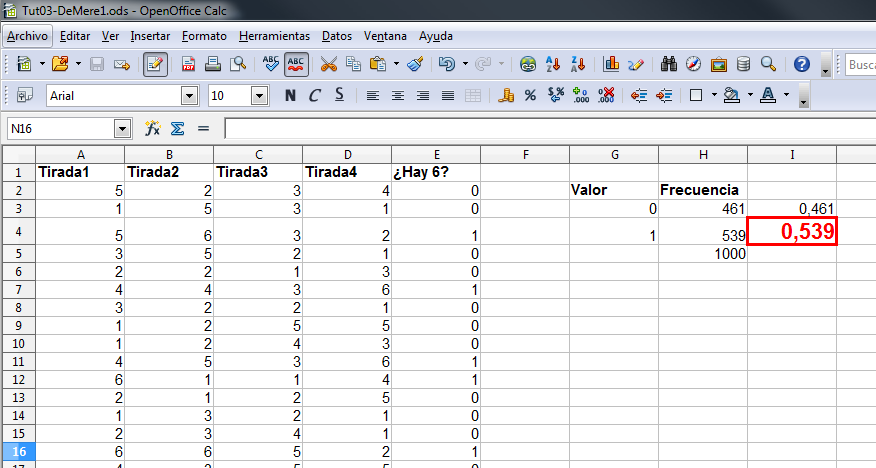
\includegraphics[width=15cm]{./fig/Tut03-41.png}
\end{center}
\caption{El fichero {\tt Cap03-DeMere1.ods} de Calc}
\label{tut03:fig:Cap03-DeMere1.ods}
\end{figure}
Las primeras cuatro columnas de la hoja de cálculo (de la {\tt A} a la {\tt D}) se han obtenido usando la función {\tt ALEATORIO.ENTRE}. Cada fila, por tanto se corresponde con una jugada, y si examinas el fichero verás que hemos jugado $1000$ veces.  Además, cada vez que pulses {\tt Ctrl+Mayús+F9} obtendrás $1000$ nuevas partidas de este juego. La columna {\tt E} contiene
un $1$ si hemos obtenido (al menos) un $6$ en las cuatro tiradas, y un $0$ si no es así. No queremos entretenernos demasiado en la forma en la que hemos conseguido que Calc haga esto, porque haremos cosas más  sofisticadas con R, de una manera muy sencilla, y merece la pena reservar nuestras fuerzas para ese empeño. Pero si sientes curiosidad, puedes hacer clic sobre la celda {\tt E2}, y ver los comandos de Calc que hemos usado para conseguirlo:
     \begin{verbatim}
=SI(O(A2=6;B2=6;C2=6;D2=6);1;0)
\end{verbatim}
Esencialmente, lo que hemos dicho, en el lenguaje de Calc, es ''Si alguna de las celdas {\tt A2, B2, C2, D2} contiene un 6, entonces el resultado es $1$. En caso contrario, es un $0$''. Y para eso hemos usado dos funciones de Calc, llamadas {\tt SI} y {\tt O}.

Las columnas {\tt G, H} e {\tt I} contienen el análisis de los resultados en forma de tabla de frecuencias y frecuencias relativas. Las frecuencias relativas son las cantidades que debemos comparar con las probabilidades calculadas de forma teórica, para saber si la teoría de las probabilidades que estamos aplicando es una descripción correcta del fenómeno. Y, en este ejemplo en particular, el resultado nos indica que la teoría del Caballero de Méré no está funcionando.

Recuerda que, según hemos visto en la teoría del curso, la ganancia que el Caballero de Méré esperaba era de un 66\% de lo invertido. Y lo que se observa es que la proporción de apuestas perdidas frente a apuestas ganadas es mucho menor de lo que el Cabllero esperaba.

En la Figura \ref{tut03:fig:Cap03-DeMere2.ods} puedes ver el comienzo del fichero correspondiente al segundo juego del Caballero de Méré. Sin entrar en muchos detalles (¡explora tú mismo el fichero!), las columnas de la izquierda contienen los resultados de las tiradas, que son números del $1$ al $36$, donde el $1$ corresponde a $(1,1)$ y $36$ corresponde a $(6,6)$. Y a la derecha aparece la tabla de frecuencias relativas, que muestra que el resultado es claramente distinto del que hemos obtenido en el otro juego. De hecho, la probabilidad de ganar en este segundo juego es aún más baja que en el otro (es aproximadamente igual a $0.49$). Usa {\tt Ctrl+Mayús+F9} unas cuantas veces para comprobarlo. Y recuerda que el Caballero de Méré creía que la probabilidad de ganar era la misma en ambos juegos.
\begin{figure}[h!]
\begin{center}
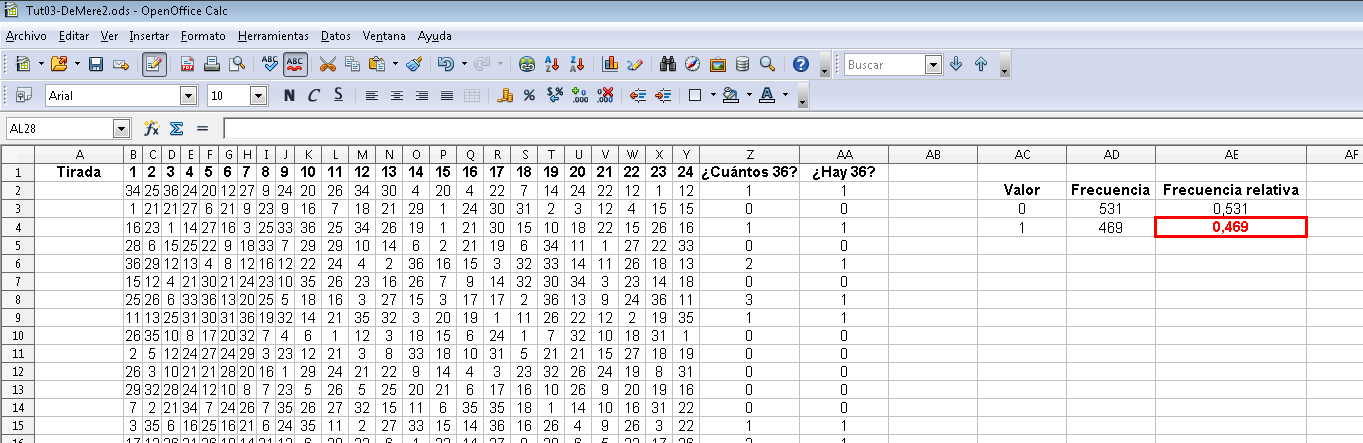
\includegraphics[width=15cm]{./fig/Tut03-42.png}
\end{center}
\caption{El fichero {\tt Cap03-DeMere2.ods} de Calc}
\label{tut03:fig:Cap03-DeMere2.ods}
\end{figure}
En la página \pageref{curso-cap03:subsubsec:JuegosDeMereCombinatoria} del Capítulo \ref{curso-cap:Probabilidad} del libro se explica cómo calcular las probabilidades correctas para ambos juegos y, más adelante en este tutorial, daremos los detalles computacionales necesarios.

\subsection{Probabilidades y la función {\tt sample} de R.}

Vamos a empezar recordando algo de lo que hemos aprendido sobre la función {\tt sample}. Si queremos fabricar $100$ números (pseudo)aleatorios entre $20$ y $80$, usaríamos (como hemos visto en la Sección \ref{tut02-tut02:subsec:NumerosAleatoriosRSample} del Tutorial-02) un código similar a este:
\begin{knitrout}
\definecolor{shadecolor}{rgb}{0.969, 0.969, 0.969}\color{fgcolor}\begin{kframe}
\begin{alltt}
\hlkwd{set.seed}\hlstd{(}\hlnum{2014}\hlstd{)}
\hlstd{n}\hlkwb{=}\hlnum{100}
\hlstd{(datos} \hlkwb{=} \hlkwd{sample}\hlstd{(}\hlnum{20}\hlopt{:}\hlnum{80}\hlstd{, n,} \hlkwc{replace}\hlstd{=}\hlnum{TRUE}\hlstd{))}
\end{alltt}
\begin{verbatim}
##   [1] 37 30 58 38 53 25 75 56 26 29 58 23 56 55 59 44 61 23 80 32 72 61 51
##  [24] 70 59 79 46 50 34 80 70 42 46 22 78 60 53 64 65 63 53 33 72 33 76 59
##  [47] 43 70 52 70 80 62 79 31 58 26 26 57 75 31 68 45 55 77 62 65 24 34 46
##  [70] 55 54 65 69 40 62 61 43 27 28 32 28 43 71 78 48 33 43 44 33 48 55 71
##  [93] 22 31 51 55 48 38 31 25
\end{verbatim}
\end{kframe}
\end{knitrout}
     (Habrás observado que el formato del código R en este Tutorial es distinto, como ya advertimos al final  del Tutorial02). De esta forma los resultados quedan guardados en el vector {\tt datos}. Los valores que hemos obtenido son reproducibles (puedes eliminar o comentar la línea con {\tt set.seed} para evitar esto). Y además, todos los números entre $20$ y $80$ son equiprobables. Y, puesto que estamos hablando de Probabilidad, es en este último aspecto en el que nos vamos a concentrar.

¿Cómo podemos fabricar valores que no sean equiprobables? En el Tutorial-02 nos las ingeniamos para conseguirlo por el procedimiento de aplicar {\tt sample} a vectores en los que había elementos repetidos. Recuerda el ejemplo:
\begin{knitrout}
\definecolor{shadecolor}{rgb}{0.969, 0.969, 0.969}\color{fgcolor}\begin{kframe}
\begin{alltt}
\hlstd{muchosUnos} \hlkwb{=} \hlkwd{c}\hlstd{(}\hlnum{1}\hlstd{,}\hlnum{1}\hlstd{,}\hlnum{1}\hlstd{,}\hlnum{1}\hlstd{,}\hlnum{1}\hlstd{,}\hlnum{1}\hlstd{,}\hlnum{1}\hlstd{,}\hlnum{1}\hlstd{,}\hlnum{1}\hlstd{,}\hlnum{2}\hlstd{)}
\hlstd{(muestra} \hlkwb{=} \hlkwd{sample}\hlstd{(muchosUnos,} \hlkwc{size}\hlstd{=}\hlnum{100}\hlstd{,} \hlkwc{replace}\hlstd{=}\hlnum{TRUE}\hlstd{) )}
\end{alltt}
\begin{verbatim}
##   [1] 1 1 1 1 1 1 1 1 1 2 1 1 1 2 1 1 1 1 1 1 1 2 1 1 1 2 1 1 1 1 2 1 1 1 1
##  [36] 1 2 1 1 1 1 1 1 1 1 1 1 1 1 1 2 1 1 1 2 1 1 2 1 1 1 1 1 1 1 1 1 1 1 1
##  [71] 1 1 1 1 1 1 1 1 1 1 1 1 1 2 1 1 1 1 1 1 1 1 1 1 2 1 1 1 1 2
\end{verbatim}
\end{kframe}
\end{knitrout}
     
     % \begin{verbatim}
%         muchosUnos = c(1,1,1,1,1,1,1,1,1,1,2)
%         (muestra = sample(muchosUnos, size=100, replace=TRUE) )
% \end{verbatim}
Este método, combinado con la función {\tt rep}, nos podría servir para conseguir lo que queremos. Pero no resulta una forma cómoda de trabajar, en cuanto las cosas sean un poco más complicadas.

\begin{ejercicio}
\label{tut03:ejercicio01}
\quad\\
Una caja contiene $100$ fichas, idénticas salvo por el número que aparece en ellas. De ellas, $35$ fichas están marcadas con el número $1$, $15$ con el número $2$, $10$ con el número $3$, $10$ con el número $4$ y el resto con el número $5$. Queremos extraer 20 fichas de la caja:
     \begin{itemize}
\item[(a)] con reemplazamiento.
\item[(b)] sin reemplazamiento.
\end{itemize}
\begin{enumerate}
\item Escribe el código en R que permite obtener esas $20$ fichas, usando las funciones {\tt rep} y {\tt sample}. Los resultados, para los casos (a) y (b), se guardaran en dos vectores, llamados {\tt sorteo1} y  {\tt sorteo2}, respectivamente. Utiliza {\tt set.seed(2014)} como primera línea de tu código, para poder comparar tus resultados con los nuestros.
\item Obtén las tablas de frecuencias absolutas y relativas de ambos vectores.
\end{enumerate}
Solución en la página \pageref{tut03:ejercicio01:sol}.
\qed
\end{ejercicio}

Pero la función {\tt sample} nos permite conseguir eso mismo de una manera mucho más sencilla. Podemos añadir a {\tt sample} un argumento opcional {\tt prob}, que es un vector con las probabilidades de cada uno de los elementos entre los que elegimos. Por ejemplo, en el vector {\tt muchosUnos}, teníamos $9$ repeticiones de $1$ por una sola de $2$. Eso significa que la probabilidad de que, al elegir un elemento al azar, sea un $1$, es
\[p_1=\dfrac{9}{10},\]
mientras que la probabilidad de que sea un $2$ es:
     \[p_2=\dfrac{1}{10}.\]
Teniendo estas probabilidades en cuenta, para elegir 100 elementos al azar podemos hacer, como antes:
\begin{knitrout}
\definecolor{shadecolor}{rgb}{0.969, 0.969, 0.969}\color{fgcolor}\begin{kframe}
\begin{alltt}
\hlkwd{set.seed}\hlstd{(}\hlnum{2014}\hlstd{)}
\hlstd{(muestra} \hlkwb{=} \hlkwd{sample}\hlstd{(muchosUnos,} \hlkwc{size}\hlstd{=}\hlnum{100}\hlstd{,} \hlkwc{replace}\hlstd{=}\hlnum{TRUE}\hlstd{) )}
\end{alltt}
\begin{verbatim}
##   [1] 1 1 1 1 1 1 2 1 1 1 1 1 1 1 1 1 1 1 2 1 1 1 1 1 1 2 1 1 1 2 1 1 1 1 2
##  [36] 1 1 1 1 1 1 1 1 1 2 1 1 1 1 1 2 1 2 1 1 1 1 1 2 1 1 1 1 2 1 1 1 1 1 1
##  [71] 1 1 1 1 1 1 1 1 1 1 1 1 1 2 1 1 1 1 1 1 1 1 1 1 1 1 1 1 1 1
\end{verbatim}
\begin{alltt}
\hlkwd{which}\hlstd{(muestra}\hlopt{==}\hlnum{2}\hlstd{)}
\end{alltt}
\begin{verbatim}
##  [1]  7 19 26 30 35 45 51 53 59 64 84
\end{verbatim}
\end{kframe}
\end{knitrout}
     Hemos incluido la función {\tt which}, para que puedas ver las posiciones que ocupan los doses en este vector. La nueva forma de conseguir esto que vamos a aprender consiste en partir de un vector con una única aparición del $1$ y el $2$, sobre el que vamos a usar directamente el argumento {\tt prob} de {\tt sample}. Así:
\begin{knitrout}
\definecolor{shadecolor}{rgb}{0.969, 0.969, 0.969}\color{fgcolor}\begin{kframe}
\begin{alltt}
\hlkwd{set.seed}\hlstd{(}\hlnum{2014}\hlstd{)}
\hlstd{(muestra} \hlkwb{=} \hlkwd{sample}\hlstd{(}\hlkwd{c}\hlstd{(}\hlnum{1}\hlstd{,}\hlnum{2}\hlstd{),} \hlkwc{size}\hlstd{=}\hlnum{100}\hlstd{,} \hlkwc{replace}\hlstd{=}\hlnum{TRUE}\hlstd{,} \hlkwc{prob}\hlstd{=}\hlkwd{c}\hlstd{(}\hlnum{9}\hlopt{/}\hlnum{10}\hlstd{,} \hlnum{1}\hlopt{/}\hlnum{10}\hlstd{) ) )}
\end{alltt}
\begin{verbatim}
##   [1] 1 1 1 1 1 1 2 1 1 1 1 1 1 1 1 1 1 1 2 1 1 1 1 1 1 2 1 1 1 2 1 1 1 1 2
##  [36] 1 1 1 1 1 1 1 1 1 2 1 1 1 1 1 2 1 2 1 1 1 1 1 2 1 1 1 1 2 1 1 1 1 1 1
##  [71] 1 1 1 1 1 1 1 1 1 1 1 1 1 2 1 1 1 1 1 1 1 1 1 1 1 1 1 1 1 1
\end{verbatim}
\begin{alltt}
\hlkwd{which}\hlstd{(muestra}\hlopt{==}\hlnum{2}\hlstd{)}
\end{alltt}
\begin{verbatim}
##  [1]  7 19 26 30 35 45 51 53 59 64 84
\end{verbatim}
\end{kframe}
\end{knitrout}
     Como ves, {\tt which} nos confirma que las posiciones son las mismas en los dos casos, así que los métodos son equivalentes. (Recuerda siempre que {\tt sample} trabaja con las posiciones del vector, y no con sus contenidos.)

\subsubsection{De Méré en R, primera visita.}
\label{tut03:subsubsec:DeMereRPrimeraVisita}

Para cerrar este apartado y preparar la discusión del siguiente, vamos a pedirle al lector que vuelva un momento a pensar en la Figura \ref{tut03:fig:Cap03-DeMere1.ods} (pág. \pageref{tut03:fig:Cap03-DeMere1.ods}). La tabla del fichero {\tt Cap03-DeMere1.ods} de Calc representa el resultado de $1000$ partidas del primer juego del Caballero de Méré. En ese juego, nosotros agrupamos cuatro tiradas del dado y las llamamos {\em una partida} del juego. Pero, en el fondo, esa tabla significa que hemos tirado el dado $4\cdot 1000$ veces en total. Y eso es algo que ya sabemos hacer en R, usando la función {\tt sample}:
\begin{knitrout}
\definecolor{shadecolor}{rgb}{0.969, 0.969, 0.969}\color{fgcolor}\begin{kframe}
\begin{alltt}
\hlkwd{set.seed}\hlstd{(}\hlnum{2014}\hlstd{)}
\hlstd{dado4000} \hlkwb{=} \hlkwd{sample}\hlstd{(}\hlnum{1}\hlopt{:}\hlnum{6}\hlstd{,} \hlnum{4000}\hlstd{,} \hlkwc{replace}\hlstd{=}\hlnum{TRUE}\hlstd{)}
\end{alltt}
\end{kframe}
\end{knitrout}
     Naturalmente, al hacer esto, R fabrica un {\em vector} de longitud 4000, en el que no resulta evidente la estructura en {\em partidas} del juego. Los matemáticos se encuentran a menudo con esta situación en la que tenemos un vector de números con alguna estructura adicional. Y han inventado el lenguaje de las matrices para poder trabajar con algunas de esas situaciones. Por ejemplo,
los primeros ocho números del vector {\tt dado4000} son:
\begin{knitrout}
\definecolor{shadecolor}{rgb}{0.969, 0.969, 0.969}\color{fgcolor}\begin{kframe}
\begin{alltt}
\hlkwd{head}\hlstd{(dado4000,} \hlnum{8}\hlstd{)}
\end{alltt}
\begin{verbatim}
## [1] 2 2 4 2 4 1 6 4
\end{verbatim}
\end{kframe}
\end{knitrout}
     pero si queremos verlos como las primeras dos partidas que hemos jugado, lo mejor es colocarlos en forma de matriz, así:
     \[
          \left(
               \begin{array}{cccc}
               2& 2& 4& 2\\
               4& 1& 6& 4
               \end{array}
               \right)
          \]
Este objeto es una matriz con dos filas y cuatro columnas. En R podemos hacer algo muy parecido, convirtiendo un vector en una matriz. Sólo tenemos que decirle a R cuál es el vector, cuántas filas o columnas tiene la matriz resultante, y cuál es el orden en que se colocan los elementos (por filas o por columnas). Para fabricar la matriz anterior hacemos:
\begin{knitrout}
\definecolor{shadecolor}{rgb}{0.969, 0.969, 0.969}\color{fgcolor}\begin{kframe}
\begin{alltt}
\hlstd{(dosPartidas} \hlkwb{=} \hlkwd{matrix}\hlstd{(} \hlkwd{head}\hlstd{(dado4000,} \hlnum{8}\hlstd{),} \hlkwc{ncol}\hlstd{=}\hlnum{4}\hlstd{,} \hlkwc{byrow}\hlstd{=}\hlnum{TRUE}\hlstd{))}
\end{alltt}
\begin{verbatim}
##      [,1] [,2] [,3] [,4]
## [1,]    2    2    4    2
## [2,]    4    1    6    4
\end{verbatim}
\begin{alltt}
\hlkwd{class}\hlstd{(dosPartidas)}
\end{alltt}
\begin{verbatim}
## [1] "matrix"
\end{verbatim}
\end{kframe}
\end{knitrout}
     La opción {\tt ncol} es el número columnas, mientras que {\tt byrow} debe su nombre al término inglés para fila, que es {\em row}.  Hemos usado la función {\tt class} para que veas que el objeto {\tt dosPartidas} es de tipo {\tt matrix}, una nueva clase de objetos de R. Fíjate también en la forma en la que R muestra esa matriz, indicando entre corchetes el número de fila (a la izquierda) y el número de columna (en la parte superior). En la próxima sección vamos a aprender el manejo básico de las matrices en R, y después retomaremos la discusión de los problemas del Caballero de Méré en R. Despedimos esta sección con un ejercicio.
\begin{ejercicio}
\label{tut03:ejercicio02}
\quad
\begin{itemize}
\item ¿Qué sucede si ejecutas el mismo código pero con {\tt byrow=FALSE}?
\item ¿Cuál es el valor {\em por defecto} de {\tt byrow}? Es decir, ¿qué sucede si no incluyes un valor de {\tt byrow}?
\end{itemize}
Solución en la página \pageref{tut03:ejercicio02:sol}. Recuerda que el ejercicio te resultará mucho más útil si te esfuerzas en resolverlo, sin mirar la solución demasiado pronto.
\qed
\end{ejercicio}


\section{Matrices en R, un primer contacto}
\label{tut03:subsec:MatricesR}
%\label{tut05:sec:MatricesR}

Las matrices son una de las formas que utiliza R para almacenar y organizar la información. A este tipo de objetos (vectores, matrices, tablas, etc.) los informáticos los conocen como Estructuras de Datos. Hemos presentado el primer ejemplo de matriz tratando de hacer visible el hecho de que la diferencia entre un vector y una matriz es, precisamente, una cuestión de {\em estructura}.

Para trabajar sobre un ejemplo concreto, vamos a colocar los números del 1 al 36 en una matriz de R, llamada {\tt M}, de 4 filas y 9 columnas (diremos que es una matriz $4\times 9$). El código es este:
\begin{knitrout}
\definecolor{shadecolor}{rgb}{0.969, 0.969, 0.969}\color{fgcolor}\begin{kframe}
\begin{alltt}
\hlstd{(M} \hlkwb{=} \hlkwd{matrix}\hlstd{(}\hlnum{1}\hlopt{:}\hlnum{36}\hlstd{,} \hlkwc{nrow}\hlstd{=}\hlnum{4}\hlstd{) )}
\end{alltt}
\begin{verbatim}
##      [,1] [,2] [,3] [,4] [,5] [,6] [,7] [,8] [,9]
## [1,]    1    5    9   13   17   21   25   29   33
## [2,]    2    6   10   14   18   22   26   30   34
## [3,]    3    7   11   15   19   23   27   31   35
## [4,]    4    8   12   16   20   24   28   32   36
\end{verbatim}
\end{kframe}
\end{knitrout}
     Como ya hemos visto antes, R rellena la matriz columna por columna.

\begin{ejercicio}
\label{tut03:ejercicio03}
\quad
Cambia el código para que la matriz $M$ se rellene fila por fila. Asegúrate, antes de seguir, de que la primera fila de la matriz M la forman los números $1$ a $9$. Solución en la página \pageref{tut03:ejercicio03:sol}.
\qed
\end{ejercicio}

     \begin{center}
\textcolor{red}{\Large\bf  ¡No sigas, si no has hecho este ejercicio!}
\end{center}
\newpage

El resultado de ese ejercicio es que ahora la matriz {\tt M} es así:
\begin{knitrout}
\definecolor{shadecolor}{rgb}{0.969, 0.969, 0.969}\color{fgcolor}\begin{kframe}
\begin{alltt}
\hlstd{M}
\end{alltt}
\begin{verbatim}
##      [,1] [,2] [,3] [,4] [,5] [,6] [,7] [,8] [,9]
## [1,]    1    2    3    4    5    6    7    8    9
## [2,]   10   11   12   13   14   15   16   17   18
## [3,]   19   20   21   22   23   24   25   26   27
## [4,]   28   29   30   31   32   33   34   35   36
\end{verbatim}
\end{kframe}
\end{knitrout}
     En R podemos cambiar las dimensiones de una matriz ya definida, usando la función {\tt dim}. Por ejemplo:
\begin{knitrout}
\definecolor{shadecolor}{rgb}{0.969, 0.969, 0.969}\color{fgcolor}\begin{kframe}
\begin{alltt}
\hlkwd{dim}\hlstd{(M)}\hlkwb{=}\hlkwd{c}\hlstd{(}\hlnum{3}\hlstd{,}\hlnum{12}\hlstd{)}
\hlstd{M}
\end{alltt}
\begin{verbatim}
##      [,1] [,2] [,3] [,4] [,5] [,6] [,7] [,8] [,9] [,10] [,11] [,12]
## [1,]    1   28   20   12    4   31   23   15    7    34    26    18
## [2,]   10    2   29   21   13    5   32   24   16     8    35    27
## [3,]   19   11    3   30   22   14    6   33   25    17     9    36
\end{verbatim}
\end{kframe}
\end{knitrout}
     El resultado demuestra que R ha redistribuido los 24 elementos de la matriz en 3 filas y 12 columnas, como le habíamos pedido. Dos observaciones sobre ese proceso:
     \begin{itemize}
\item Para redistribuir los elementos R ha trabajado, de nuevo, por columnas (es su modo por defecto, recuérdalo). Es decir, que la primera columna de la matriz redimensionada la forman los tres primeros elementos de la primera columna de M (antes de la redimensión), que eran el $1, 10$ y el $19$. Si avanzas así, por columnas, es fácil ver el esquema que R ha usado para redistribuir los números (y si miras las diagonales verás los restos del orden original).
\item Cuidado: aunque el procedimiento es reversible, al hacer esto hemos cambiado la {\em estructura} de la matriz original.
\end{itemize}

\begin{ejercicio}
\label{tut03:ejercicio04}
\quad
Devuelve la matriz M a la forma anterior, en la que la primera fila la forman los números $1$ a $9$. Solución en la página \pageref{tut03:ejercicio04:sol}.
\qed
\end{ejercicio}

     \vspace{1cm}
\begin{center}
\textcolor{red}{\Large\bf  ¡No sigas, si no has hecho este ejercicio!}
\end{center}

Además de cambiar la dimensión, la función {\tt dim} sirve para {\em obtener} esa dimensión (en forma de vector de dos elementos, número de filas y columnas respectivamente.) Por ejemplo (si has hecho el Ejercicio \ref{tut03:ejercicio03}):
\begin{knitrout}
\definecolor{shadecolor}{rgb}{0.969, 0.969, 0.969}\color{fgcolor}\begin{kframe}
\begin{alltt}
\hlkwd{dim}\hlstd{(M)}
\end{alltt}
\begin{verbatim}
## [1] 4 9
\end{verbatim}
\end{kframe}
\end{knitrout}
     
     \begin{ejercicio}
\label{tut03:ejercicio05}
\quad
¿Cuanto vale la dimensión de un vector? Define un vector con $10$ elementos (por ejemplo, {\tt 1:10}) y calcula su dimensión.
Solución en la página \pageref{tut03:ejercicio05:sol}.
\qed
\end{ejercicio}

Como ilustra el próximo ejercicio, las matrices no tienen por qué ser numéricas.
\begin{ejercicio}
\label{tut03:ejercicio06}
\quad
Construye una matriz $4\times 3$ con las primeras 12 letras del alfabeto (recuerda el vector {\tt letters}), de manera que la primera fila sea {\tt a b c}. Comprueba su dimensión, y después cámbiala para obtener una matriz $3\times 4$.
Solución en la página \pageref{tut03:ejercicio06:sol}.
\qed
\end{ejercicio}


\subsection{Funciones matriciales y operaciones con matrices en R.}
\label{tut03:subsec:FuncionesMatricialesR}

La función {\tt dim} es sólo el primer ejemplo que hemos encontrado de una función matricial. Pero hay muchas otras. Por ejemplo, si queremos trasponer una matriz, cambiando filas por columnas, usaremos la función {\tt t} (su nombre es la letra {\tt t}). Al aplicarla a la matriz {\tt M} se obtiene:
\begin{knitrout}
\definecolor{shadecolor}{rgb}{0.969, 0.969, 0.969}\color{fgcolor}\begin{kframe}
\begin{alltt}
\hlkwd{t}\hlstd{(M)}
\end{alltt}
\begin{verbatim}
##       [,1] [,2] [,3] [,4]
##  [1,]    1   10   19   28
##  [2,]    2   11   20   29
##  [3,]    3   12   21   30
##  [4,]    4   13   22   31
##  [5,]    5   14   23   32
##  [6,]    6   15   24   33
##  [7,]    7   16   25   34
##  [8,]    8   17   26   35
##  [9,]    9   18   27   36
\end{verbatim}
\end{kframe}
\end{knitrout}
     Al trasponer una matriz $m\times n$ se obtiene una matriz $n\times m$. Pero fíjate en que el efecto de trasponer una matriz $m\times n$ no es lo mismo que redimensionar la matriz para que sus dimensiones sean $n\times m$. El siguiente ejercicio lo demuestra.

\begin{ejercicio}
\label{tut03:ejercicio07}
\quad
Dada la matriz
\begin{knitrout}
\definecolor{shadecolor}{rgb}{0.969, 0.969, 0.969}\color{fgcolor}\begin{kframe}
\begin{alltt}
     \hlstd{(W} \hlkwb{=} \hlkwd{matrix}\hlstd{(}\hlnum{1}\hlopt{:}\hlnum{15}\hlstd{,} \hlkwc{nrow}\hlstd{=}\hlnum{3}\hlstd{,} \hlkwc{byrow}\hlstd{=}\hlnum{TRUE}\hlstd{))}
\end{alltt}
\begin{verbatim}
##      [,1] [,2] [,3] [,4] [,5]
## [1,]    1    2    3    4    5
## [2,]    6    7    8    9   10
## [3,]   11   12   13   14   15
\end{verbatim}
\end{kframe}
\end{knitrout}
     comprueba que esta operación:
\begin{knitrout}
\definecolor{shadecolor}{rgb}{0.969, 0.969, 0.969}\color{fgcolor}\begin{kframe}
\begin{alltt}
\hlkwd{t}\hlstd{(W)}
\end{alltt}
\end{kframe}
\end{knitrout}
     y esta
\begin{knitrout}
\definecolor{shadecolor}{rgb}{0.969, 0.969, 0.969}\color{fgcolor}\begin{kframe}
\begin{alltt}
     \hlkwd{dim}\hlstd{(W)} \hlkwb{=} \hlkwd{c}\hlstd{(}\hlnum{5}\hlstd{,}\hlnum{3}\hlstd{)}
\end{alltt}
\end{kframe}
\end{knitrout}
     no dan el mismo resultado. Solución en la página \pageref{tut03:ejercicio07:sol}.
\qed
\end{ejercicio}
Otras dos funciones matriciales útiles son {\tt nrow} y {\tt ncol}, que proporcionan, respectivamente, el número de filas y columnas de la matriz. Con la matriz {\tt M}, por ejemplo:
\begin{knitrout}
\definecolor{shadecolor}{rgb}{0.969, 0.969, 0.969}\color{fgcolor}\begin{kframe}
\begin{alltt}
\hlkwd{nrow}\hlstd{(M)}
\end{alltt}
\begin{verbatim}
## [1] 4
\end{verbatim}
\begin{alltt}
\hlkwd{ncol}\hlstd{(M)}
\end{alltt}
\begin{verbatim}
## [1] 9
\end{verbatim}
\end{kframe}
\end{knitrout}
     Para las matrices numéricas existen, además, cuatro funciones que permiten hacer operaciones por sumas o por columnas. Por ejemplo, la función {\tt rowSums} calcula la suma de cada una de las filas, mientras que {\tt sumCols} hace lo propio con las columnas:
\begin{knitrout}
\definecolor{shadecolor}{rgb}{0.969, 0.969, 0.969}\color{fgcolor}\begin{kframe}
\begin{alltt}
\hlkwd{rowSums}\hlstd{(M)}
\end{alltt}
\begin{verbatim}
## [1]  45 126 207 288
\end{verbatim}
\begin{alltt}
\hlkwd{colSums}\hlstd{(M)}
\end{alltt}
\begin{verbatim}
## [1] 58 62 66 70 74 78 82 86 90
\end{verbatim}
\end{kframe}
\end{knitrout}
     Las funciones {\tt rowMeans} y {\tt colMeans} proporcionan las medias aritméticas por filas y por columnas, respectivamente.

Hay muchas otras operaciones matriciales y, más adelante, iremos conociendo algunas. En la Sección \ref{tut03:subsec:IntroAlgebraMatricial} (pág. \pageref{tut03:subsec:IntroAlgebraMatricial}) hemos añadido un apartado opcional con algo más de información, para aquellos lectores que estén algo más familiarizados con el álgebra matricial (multiplicación de matrices, determinantes, inversas y operaciones relacionadas con estas). Pero hay una estrategia general cuando queremos aplicar una función a todas las filas (o columnas) de una matriz, que consiste en utilizar la función {\tt apply}. Esta función usa (al menos) tres argumentos: la matriz, un índice que puede valer $1$ o $2$ para indicar filas o columnas, respectivamente, y la función que deseamos aplicar. Por ejemplo, dada la matriz {\tt M} que venimos usando, puedes usar {\tt apply} para calcular las sumas de las filas y columnas, mediante estos comandos:
\begin{knitrout}
\definecolor{shadecolor}{rgb}{0.969, 0.969, 0.969}\color{fgcolor}\begin{kframe}
\begin{alltt}
\hlcom{# Por filas:}
\hlkwd{apply}\hlstd{(M,} \hlnum{1}\hlstd{, sum)}
\end{alltt}
\begin{verbatim}
## [1]  45 126 207 288
\end{verbatim}
\begin{alltt}
\hlcom{# Por columnas:}
\hlkwd{apply}\hlstd{(M,} \hlnum{2}\hlstd{, sum)}
\end{alltt}
\begin{verbatim}
## [1] 58 62 66 70 74 78 82 86 90
\end{verbatim}
\end{kframe}
\end{knitrout}
     Y puedes comprobar que estos son los mismos resultados que obtuvimos con {\tt rowSums} y {\tt colSums}, respectivamente.
\begin{ejercicio}
\label{tut03:ejercicio07a}
\quad
\begin{enumerate}
\item Calcula la cuasidesviación típica muestral de las filas de {\tt M}.
\item Calcula la mediana de las columnas de {\tt M}.
\item La cuasidesviación típica muestral y la mediana son números. Pero también hay funciones que devuelven vectores en lugar de números. ¿Qué sucede si usas {\tt apply} para aplicar la función {\tt summary} a las columnas de {\tt M}?
\end{enumerate}
Soluciones en la página \pageref{tut03:ejercicio07a:sol}.
\qed
\end{ejercicio}


\subsection{Operaciones elemento a elemento.}
\label{tut03:subsec:OperacionesElementoAElementoMatrices}


Otra propiedad interesante de las matrices es que podemos operar con ellas de forma muy parecida a como hemos hecho con los vectores. Para disponer de un ejemplo, este código define un par de matrices {\tt A} y {\tt B}, ambas matrices aleatorias (construidas con sample) de dimensión $3\times 4$.
\begin{knitrout}
\definecolor{shadecolor}{rgb}{0.969, 0.969, 0.969}\color{fgcolor}\begin{kframe}
\begin{alltt}
     \hlkwd{set.seed}\hlstd{(}\hlnum{2014}\hlstd{)}
\hlstd{(A} \hlkwb{=} \hlkwd{matrix}\hlstd{(}\hlkwd{sample}\hlstd{(}\hlopt{-}\hlnum{10}\hlopt{:}\hlnum{10}\hlstd{,} \hlnum{12}\hlstd{,} \hlkwc{replace}\hlstd{=}\hlnum{TRUE}\hlstd{),} \hlkwc{nrow}\hlstd{=}\hlnum{3}\hlstd{))}
\end{alltt}
\begin{verbatim}
##      [,1] [,2] [,3] [,4]
## [1,]   -4   -4    9   -7
## [2,]   -7    1    2    3
## [3,]    3   -9   -8   -9
\end{verbatim}
\begin{alltt}
\hlstd{(B} \hlkwb{=} \hlkwd{matrix}\hlstd{(}\hlkwd{sample}\hlstd{(}\hlopt{-}\hlnum{10}\hlopt{:}\hlnum{10}\hlstd{,} \hlnum{12}\hlstd{,} \hlkwc{replace}\hlstd{=}\hlnum{TRUE}\hlstd{),} \hlkwc{nrow}\hlstd{=}\hlnum{3}\hlstd{))}
\end{alltt}
\begin{verbatim}
##      [,1] [,2] [,3] [,4]
## [1,]    2   -2   10    4
## [2,]    2    4   -6    0
## [3,]    3   -9    8    7
\end{verbatim}
\end{kframe}
\end{knitrout}
     Y ahora podemos ilustrar algunas operaciones con estas matrices. Por ejemplo, podemos multiplicar {\tt A } por $2$:
\begin{knitrout}
\definecolor{shadecolor}{rgb}{0.969, 0.969, 0.969}\color{fgcolor}\begin{kframe}
\begin{alltt}
\hlnum{2} \hlopt{*} \hlstd{A}
\end{alltt}
\begin{verbatim}
##      [,1] [,2] [,3] [,4]
## [1,]   -8   -8   18  -14
## [2,]  -14    2    4    6
## [3,]    6  -18  -16  -18
\end{verbatim}
\end{kframe}
\end{knitrout}
     Podemos elevar {\tt B} al cuadrado:
\begin{knitrout}
\definecolor{shadecolor}{rgb}{0.969, 0.969, 0.969}\color{fgcolor}\begin{kframe}
\begin{alltt}
\hlstd{B}\hlopt{^}\hlnum{2}
\end{alltt}
\begin{verbatim}
##      [,1] [,2] [,3] [,4]
## [1,]    4    4  100   16
## [2,]    4   16   36    0
## [3,]    9   81   64   49
\end{verbatim}
\end{kframe}
\end{knitrout}
     Podemos sumar las matrices:
\begin{knitrout}
\definecolor{shadecolor}{rgb}{0.969, 0.969, 0.969}\color{fgcolor}\begin{kframe}
\begin{alltt}
\hlstd{A} \hlopt{+} \hlstd{B}
\end{alltt}
\begin{verbatim}
##      [,1] [,2] [,3] [,4]
## [1,]   -2   -6   19   -3
## [2,]   -5    5   -4    3
## [3,]    6  -18    0   -2
\end{verbatim}
\end{kframe}
\end{knitrout}
     Y también podemos multiplicarlas elemento a elemento.
\begin{knitrout}
\definecolor{shadecolor}{rgb}{0.969, 0.969, 0.969}\color{fgcolor}\begin{kframe}
\begin{alltt}
     \hlstd{A} \hlopt{*} \hlstd{B}
\end{alltt}
\begin{verbatim}
##      [,1] [,2] [,3] [,4]
## [1,]   -8    8   90  -28
## [2,]  -14    4  -12    0
## [3,]    9   81  -64  -63
\end{verbatim}
\end{kframe}
\end{knitrout}
     ¡Pero cuidado! Lo que R ha hecho aquí es lo mismo que ha hecho en todas las operaciones anteriores: trabajar elemento a elemento, como hacíamos en los vectores. En particular el resultado {\bf no es el producto de matrices} tal como se define habitualmente en Matemáticas. En la Sección \ref{tut03:subsec:IntroAlgebraMatricial} (pág. \pageref{tut03:subsec:IntroAlgebraMatricial}) veremos cómo se calcula el verdadero producto matricial.

Naturalmente, podemos aplicar una función (como, por poner un ejemplo, el arcotangente, {\tt atan}), a todos los elementos de la matriz:
\begin{knitrout}
\definecolor{shadecolor}{rgb}{0.969, 0.969, 0.969}\color{fgcolor}\begin{kframe}
\begin{alltt}
\hlkwd{atan}\hlstd{(A)}
\end{alltt}
\begin{verbatim}
##       [,1]   [,2]  [,3]  [,4]
## [1,] -1.33 -1.326  1.46 -1.43
## [2,] -1.43  0.785  1.11  1.25
## [3,]  1.25 -1.460 -1.45 -1.46
\end{verbatim}
\end{kframe}
\end{knitrout}
     Y no queremos cerrar este apartado sin comentar algo que luego nos será muy útil. Además de las operaciones aritméticas, también podemos hacer operaciones lógicas (booleanas; recuerda el Tutorial02, pág. \pageref{tut02-tut02:subsubsec:SeleccionElementosCondicionesValoresBooleanosWhich}). Si queremos saber qué elementos de la matriz {\tt A} son mayores o iguales que $0$, haremos:
\begin{knitrout}
\definecolor{shadecolor}{rgb}{0.969, 0.969, 0.969}\color{fgcolor}\begin{kframe}
\begin{alltt}
\hlstd{A} \hlopt{>=} \hlnum{0}
\end{alltt}
\begin{verbatim}
##       [,1]  [,2]  [,3]  [,4]
## [1,] FALSE FALSE  TRUE FALSE
## [2,] FALSE  TRUE  TRUE  TRUE
## [3,]  TRUE FALSE FALSE FALSE
\end{verbatim}
\end{kframe}
\end{knitrout}
     Y, como ves, la respuesta es una matriz de valores booleanos, con las respuestas a esa pregunta, calculados de nuevo {\em elemento a elemento}.

\begin{ejercicio}
\label{tut03:ejercicio08}
\quad
\begin{enumerate}
\item Construye una matriz de la misma dimensión que {\tt B} y con elementos {\tt TRUE/FALSE} que permita saber si el correspondiente elemento de {\tt B} son iguales a $2$.
\item Cambia la dimensión de la matriz {\tt A} para que sea una matriz $2\times 6$. Trata de calcular ahora el producto {\tt A * B}. ¿Qué sucede?
\end{enumerate}
Soluciones en la página \pageref{tut03:ejercicio08:sol}.
\qed
\end{ejercicio}

\subsection{Selección de elementos en las matrices de R.}
\label{tut03:subsec:SeleccionElementosMatrices}


La selección de elementos de una matriz de R usa técnicas parecidas a las que ya hemos aprendido en el caso de los vectores. Vamos a suponer, por ejemplo, que queremos seleccionar el elemento de la tercera fila, sexta columna de la matriz {\tt M} que venimos usando. En notación matemática, si $M$ es la matriz ese elemento sería $m_{3,6}$ (a menudo se usa una letra mayúscula para la matriz y la misma letra minúscula para sus elementos). Recuerda que la matriz era:
\begin{knitrout}
\definecolor{shadecolor}{rgb}{0.969, 0.969, 0.969}\color{fgcolor}\begin{kframe}
\begin{alltt}
\hlstd{M}
\end{alltt}
\begin{verbatim}
##      [,1] [,2] [,3] [,4] [,5] [,6] [,7] [,8] [,9]
## [1,]    1    2    3    4    5    6    7    8    9
## [2,]   10   11   12   13   14   15   16   17   18
## [3,]   19   20   21   22   23   24   25   26   27
## [4,]   28   29   30   31   32   33   34   35   36
\end{verbatim}
\end{kframe}
\end{knitrout}
     El elemento deseado se selecciona usando así los corchetes:
\begin{knitrout}
\definecolor{shadecolor}{rgb}{0.969, 0.969, 0.969}\color{fgcolor}\begin{kframe}
\begin{alltt}
\hlstd{M[}\hlnum{3}\hlstd{,} \hlnum{6}\hlstd{]}
\end{alltt}
\begin{verbatim}
## [1] 24
\end{verbatim}
\end{kframe}
\end{knitrout}
     ¿Y si lo que queremos es seleccionar una fila entera? Por ejemplo, la segunda fila. El propio R, al mostrar la matriz {\tt M}, nos da una pista sobre la forma de conseguir esto con la notación de corchetes. La forma de obtener la segunda fila es esta:
\begin{knitrout}
\definecolor{shadecolor}{rgb}{0.969, 0.969, 0.969}\color{fgcolor}\begin{kframe}
\begin{alltt}
\hlstd{M[}\hlnum{2}\hlstd{, ]}
\end{alltt}
\begin{verbatim}
## [1] 10 11 12 13 14 15 16 17 18
\end{verbatim}
\end{kframe}
\end{knitrout}
     mientras que si lo que quieres es la cuarta columna, tendrás que usar:
\begin{knitrout}
\definecolor{shadecolor}{rgb}{0.969, 0.969, 0.969}\color{fgcolor}\begin{kframe}
\begin{alltt}
\hlstd{M[ ,} \hlnum{4}\hlstd{]}
\end{alltt}
\begin{verbatim}
## [1]  4 13 22 31
\end{verbatim}
\end{kframe}
\end{knitrout}
     Esta notación con corchetes es, como ya vimos con los vectores, muy flexible. Por ejemplo, para seleccionar las columnas de la $5$ a la $8$ podemos hacer:
\begin{knitrout}
\definecolor{shadecolor}{rgb}{0.969, 0.969, 0.969}\color{fgcolor}\begin{kframe}
\begin{alltt}
\hlstd{M[ ,} \hlnum{5}\hlopt{:}\hlnum{8}\hlstd{]}
\end{alltt}
\begin{verbatim}
##      [,1] [,2] [,3] [,4]
## [1,]    5    6    7    8
## [2,]   14   15   16   17
## [3,]   23   24   25   26
## [4,]   32   33   34   35
\end{verbatim}
\end{kframe}
\end{knitrout}
     Y si lo que quieres son las columnas pares, puedes probar con:
\begin{knitrout}
\definecolor{shadecolor}{rgb}{0.969, 0.969, 0.969}\color{fgcolor}\begin{kframe}
\begin{alltt}
\hlstd{M[ ,} \hlkwd{seq}\hlstd{(}\hlkwc{from}\hlstd{=}\hlnum{2}\hlstd{,} \hlkwc{to}\hlstd{=}\hlkwd{ncol}\hlstd{(M),} \hlkwc{by}\hlstd{=}\hlnum{2}\hlstd{)]}
\end{alltt}
\begin{verbatim}
##      [,1] [,2] [,3] [,4]
## [1,]    2    4    6    8
## [2,]   11   13   15   17
## [3,]   20   22   24   26
## [4,]   29   31   33   35
\end{verbatim}
\end{kframe}
\end{knitrout}
     Fíjate en que, en este ejemplo, como sabemos el número de columnas podríamos haber escrito simplemente
\begin{knitrout}
\definecolor{shadecolor}{rgb}{0.969, 0.969, 0.969}\color{fgcolor}\begin{kframe}
\begin{alltt}
     \hlstd{M[ ,} \hlkwd{c}\hlstd{(}\hlnum{2}\hlstd{,}\hlnum{4}\hlstd{,}\hlnum{6}\hlstd{,}\hlnum{8}\hlstd{)]}
\end{alltt}
\begin{verbatim}
##      [,1] [,2] [,3] [,4]
## [1,]    2    4    6    8
## [2,]   11   13   15   17
## [3,]   20   22   24   26
## [4,]   29   31   33   35
\end{verbatim}
\end{kframe}
\end{knitrout}
     y el resultado es el mismo. Pero el método anterior tiene la ventaja de que no depende del conocimiento previo de las dimensiones de la matriz. Es una buena práctica acostumbrarse a buscar soluciones tan generales como sea posible. Aparte de hacer avanzar por la senda de la sabiduría, esto te facilitaré reutilizar el mismo código en el futuro para otras tareas.

Naturalmente, es posible combinar la selección por filas y por columnas. Supongamos que queremos los elementos de la matriz {\tt M} que ocupan la intersección de las filas $2$ y $4$ con las columnas $6$ y $9$. Los podemos obtener de esta manera:
\begin{knitrout}
\definecolor{shadecolor}{rgb}{0.969, 0.969, 0.969}\color{fgcolor}\begin{kframe}
\begin{alltt}
\hlstd{M[} \hlkwd{c}\hlstd{(}\hlnum{2}\hlstd{,} \hlnum{4}\hlstd{),} \hlkwd{c}\hlstd{(}\hlnum{6}\hlstd{,} \hlnum{9}\hlstd{)]}
\end{alltt}
\begin{verbatim}
##      [,1] [,2]
## [1,]   15   18
## [2,]   33   36
\end{verbatim}
\end{kframe}
\end{knitrout}
     
     \subsection{Matrices por filas y columnas: {\tt cbind} y {\tt rbind}.}
\label{tut03:subsec:RbindCbind}

Otra manera de fabricar matrices a partir de vectores es utilizar las funciones {\tt cbind} y {\tt rbind} (donde r y c proceden de row (fila) y column (columna), respectivamente). Estas funciones nos permiten escribir las filas o columnas directamente como vectores. Por ejemplo, podemos fabricar una matriz {\tt U} a partir de sus tres filas, definidas todas mediante vectores de la misma longitud (que en este caso, es $4$), con el código:
\begin{knitrout}
\definecolor{shadecolor}{rgb}{0.969, 0.969, 0.969}\color{fgcolor}\begin{kframe}
\begin{alltt}
\hlstd{(U} \hlkwb{=} \hlkwd{rbind}\hlstd{(}\hlnum{2}\hlopt{:}\hlnum{5}\hlstd{,} \hlnum{1}\hlopt{:}\hlnum{4}\hlstd{,} \hlkwd{c}\hlstd{(}\hlopt{-}\hlnum{2}\hlstd{,}\hlnum{1}\hlstd{,}\hlnum{4}\hlstd{,}\hlnum{7}\hlstd{)))}
\end{alltt}
\begin{verbatim}
##      [,1] [,2] [,3] [,4]
## [1,]    2    3    4    5
## [2,]    1    2    3    4
## [3,]   -2    1    4    7
\end{verbatim}
\end{kframe}
\end{knitrout}
     Y para ilustrar la función {\tt cbind} vamos a añadirle una columna más a la matriz {\tt U}, escribiendo:
\begin{knitrout}
\definecolor{shadecolor}{rgb}{0.969, 0.969, 0.969}\color{fgcolor}\begin{kframe}
\begin{alltt}
\hlstd{(U} \hlkwb{=} \hlkwd{cbind}\hlstd{(U,} \hlkwd{c}\hlstd{(}\hlnum{11}\hlstd{,}\hlnum{17}\hlstd{,}\hlopt{-}\hlnum{4}\hlstd{)))}
\end{alltt}
\begin{verbatim}
##      [,1] [,2] [,3] [,4] [,5]
## [1,]    2    3    4    5   11
## [2,]    1    2    3    4   17
## [3,]   -2    1    4    7   -4
\end{verbatim}
\end{kframe}
\end{knitrout}
     
     \begin{ejercicio}
\label{tut03:ejercicio09}
\quad
Dada la matriz
\begin{knitrout}
\definecolor{shadecolor}{rgb}{0.969, 0.969, 0.969}\color{fgcolor}\begin{kframe}
\begin{alltt}
     \hlstd{(B} \hlkwb{=} \hlkwd{matrix}\hlstd{(}\hlnum{1}\hlopt{:}\hlnum{100}\hlstd{,} \hlkwc{nrow}\hlstd{=}\hlnum{10}\hlstd{))}
\end{alltt}
\begin{verbatim}
##       [,1] [,2] [,3] [,4] [,5] [,6] [,7] [,8] [,9] [,10]
##  [1,]    1   11   21   31   41   51   61   71   81    91
##  [2,]    2   12   22   32   42   52   62   72   82    92
##  [3,]    3   13   23   33   43   53   63   73   83    93
##  [4,]    4   14   24   34   44   54   64   74   84    94
##  [5,]    5   15   25   35   45   55   65   75   85    95
##  [6,]    6   16   26   36   46   56   66   76   86    96
##  [7,]    7   17   27   37   47   57   67   77   87    97
##  [8,]    8   18   28   38   48   58   68   78   88    98
##  [9,]    9   19   29   39   49   59   69   79   89    99
## [10,]   10   20   30   40   50   60   70   80   90   100
\end{verbatim}
\end{kframe}
\end{knitrout}
     añádele a la derecha una columna que contenga los cuadrados de los elementos de la primera columna de {\tt B}. ¿Cómo la añadirías a la izquierda? ¿Y en el medio (pongamos, entre la segunda y la tercera)? Solución en la página \pageref{tut03:ejercicio09:sol}.
\qed
\end{ejercicio}

\subsection{El camino de vuelta: de matrices a vectores. El valor {\tt NULL}.}
\label{tut03:subsec:CaminoVueltaMatricesVectores}

Hemos visto que la función {\tt matrix} sirve para convertir un vector en una matriz. Pero a veces necesitaremos la transformación contraria. Afortunadamente, hay varias maneras de convertir una matriz en un vector. Para trabajar sobre un ejemplo concreto vamos a fabricar con la matriz {\tt A}, que hemos usado en anteriores ejemplos, y que habíamos fabricado así:
\begin{knitrout}
\definecolor{shadecolor}{rgb}{0.969, 0.969, 0.969}\color{fgcolor}\begin{kframe}
\begin{alltt}
\hlkwd{set.seed}\hlstd{(}\hlnum{2014}\hlstd{)}
\hlstd{(A} \hlkwb{=} \hlkwd{matrix}\hlstd{(}\hlkwd{sample}\hlstd{(}\hlopt{-}\hlnum{10}\hlopt{:}\hlnum{10}\hlstd{,} \hlnum{12}\hlstd{,} \hlkwc{replace}\hlstd{=}\hlnum{TRUE}\hlstd{),} \hlkwc{nrow}\hlstd{=}\hlnum{3}\hlstd{))}
\end{alltt}
\begin{verbatim}
##      [,1] [,2] [,3] [,4]
## [1,]   -4   -4    9   -7
## [2,]   -7    1    2    3
## [3,]    3   -9   -8   -9
\end{verbatim}
\end{kframe}
\end{knitrout}
     La forma más clara de convertirla en un vector es usando una función matricial llamada {\tt as.vector}:
\begin{knitrout}
\definecolor{shadecolor}{rgb}{0.969, 0.969, 0.969}\color{fgcolor}\begin{kframe}
\begin{alltt}
\hlkwd{as.vector}\hlstd{(A)}
\end{alltt}
\begin{verbatim}
##  [1] -4 -7  3 -4  1 -9  9  2 -8 -7  3 -9
\end{verbatim}
\end{kframe}
\end{knitrout}
     Fiel a sus costumbres, R trabaja por columnas, de manera que los primeros tres elementos del vector son los de la primera columna de {\tt A}. Si queremos fabricar el vector avanzando por filas, podemos usar la función {\tt t} para trasponer primero la matriz, y luego usar {\tt as.vector}:
\begin{knitrout}
\definecolor{shadecolor}{rgb}{0.969, 0.969, 0.969}\color{fgcolor}\begin{kframe}
\begin{alltt}
\hlkwd{as.vector}\hlstd{(}\hlkwd{t}\hlstd{(A))}
\end{alltt}
\begin{verbatim}
##  [1] -4 -4  9 -7 -7  1  2  3  3 -9 -8 -9
\end{verbatim}
\end{kframe}
\end{knitrout}
     
     Hay otra manera muy fácil de convertir matrices en vectores, usando
\begin{knitrout}
\definecolor{shadecolor}{rgb}{0.969, 0.969, 0.969}\color{fgcolor}\begin{kframe}
\begin{alltt}
     \hlkwd{c}\hlstd{(A)}
\end{alltt}
\begin{verbatim}
##  [1] -4 -7  3 -4  1 -9  9  2 -8 -7  3 -9
\end{verbatim}
\end{kframe}
\end{knitrout}
     El resultado es el mismo que con {\tt as.vector}, así que podrías pensar que es mejor (por más breve) usar la función {\tt c}. Pero a menudo, cuando escribimos programas, la claridad es más importante que la brevedad.

Finalmente, hay un método algo más esotérico para convertir una matriz en un vector, que consiste en ``borrarle'' sus dimensiones. Recuerda que para obtener las dimensiones de la matriz hacemos:
\begin{knitrout}
\definecolor{shadecolor}{rgb}{0.969, 0.969, 0.969}\color{fgcolor}\begin{kframe}
\begin{alltt}
\hlkwd{dim}\hlstd{(A)}
\end{alltt}
\begin{verbatim}
## [1] 3 4
\end{verbatim}
\end{kframe}
\end{knitrout}
     Pero también podemos usar la función {\tt dim} para {\em cambiar} esas dimensiones. Vamos a hacer esto, pero cambiando las dimensiones por el valor {\tt NULL}. Este símbolo representa un valor especial R, como otros valores especiales que ya hemos encontrado: {\tt NA, NaN, Inf}. El valor {\tt NULL} se utiliza, principalmente, para ``vaciar'' una variable. Es una forma de decirle a R ``olvídate del contenido de esta variable''. Así que si hacemos
\begin{knitrout}
\definecolor{shadecolor}{rgb}{0.969, 0.969, 0.969}\color{fgcolor}\begin{kframe}
\begin{alltt}
     \hlkwd{dim}\hlstd{(A)} \hlkwb{=} \hlkwa{NULL}
\end{alltt}
\end{kframe}
\end{knitrout}
     le estamos diciendo a R ``olvídate de que {\tt A} tenía dimensiones''. Y el resultado es que si ahora preguntamos por {\tt A} obtenemos:
\begin{knitrout}
\definecolor{shadecolor}{rgb}{0.969, 0.969, 0.969}\color{fgcolor}\begin{kframe}
\begin{alltt}
\hlstd{A}
\end{alltt}
\begin{verbatim}
##  [1] -4 -7  3 -4  1 -9  9  2 -8 -7  3 -9
\end{verbatim}
\begin{alltt}
\hlkwd{class}\hlstd{(A)}
\end{alltt}
\begin{verbatim}
## [1] "integer"
\end{verbatim}
\end{kframe}
\end{knitrout}
     Es decir, que {\tt A} ha pasado a ser un vector de tipo {\tt integer}. Los vectores, en R, no tienen dimensión. O,  mejor dicho, su dimensión es {\tt NULL}.



\subsection{Introducción al álgebra matricial en  R.}
\label{tut03:subsec:IntroAlgebraMatricial}
{\bf Esta sección es opcional.}

Esta sección no pretende ser, en modo alguno, una introducción siquiera mínimamente completa al Álgebra Lineal con R, porque eso nos ocuparía mucho más espacio del que razonablemente podemos dedicarle en este tutorial. Pero sí queremos que sirva de aperitivo para aquellos lectores con conocimientos más avanzados sobre matrices.

Para empezar, en R, el producto matricial se representa con el operador {\tt \%*\%}. Por ejemplo, si definimos las matrices:
\begin{knitrout}
\definecolor{shadecolor}{rgb}{0.969, 0.969, 0.969}\color{fgcolor}\begin{kframe}
\begin{alltt}
\hlstd{(U} \hlkwb{=} \hlkwd{matrix}\hlstd{(}\hlnum{1}\hlopt{:}\hlnum{8}\hlstd{,} \hlkwc{nrow}\hlstd{=}\hlnum{2}\hlstd{,} \hlkwc{byrow}\hlstd{=}\hlnum{TRUE}\hlstd{))}
\end{alltt}
\begin{verbatim}
##      [,1] [,2] [,3] [,4]
## [1,]    1    2    3    4
## [2,]    5    6    7    8
\end{verbatim}
\begin{alltt}
\hlstd{(V} \hlkwb{=} \hlkwd{matrix}\hlstd{(}\hlkwd{rep}\hlstd{(}\hlkwd{c}\hlstd{(}\hlnum{1}\hlstd{,}\hlopt{-}\hlnum{1}\hlstd{),}\hlnum{12}\hlstd{),} \hlkwc{nrow}\hlstd{=}\hlnum{4}\hlstd{,} \hlkwc{byrow}\hlstd{=}\hlnum{TRUE}\hlstd{))}
\end{alltt}
\begin{verbatim}
##      [,1] [,2] [,3] [,4] [,5] [,6]
## [1,]    1   -1    1   -1    1   -1
## [2,]    1   -1    1   -1    1   -1
## [3,]    1   -1    1   -1    1   -1
## [4,]    1   -1    1   -1    1   -1
\end{verbatim}
\end{kframe}
\end{knitrout}
     En este caso, $U$ es $2\times 4$, mientras que $V$ es $4\times 6$, así que el producto es esta matriz $2\times 6$:
\begin{knitrout}
\definecolor{shadecolor}{rgb}{0.969, 0.969, 0.969}\color{fgcolor}\begin{kframe}
\begin{alltt}
\hlstd{U} \hlopt \hlstd{V}
\end{alltt}
\begin{verbatim}
##      [,1] [,2] [,3] [,4] [,5] [,6]
## [1,]   10  -10   10  -10   10  -10
## [2,]   26  -26   26  -26   26  -26
\end{verbatim}
\end{kframe}
\end{knitrout}
     Naturalmente, si tratamos de hacer un producto no definido, R nos reprende con un error:
\begin{knitrout}
\definecolor{shadecolor}{rgb}{0.969, 0.969, 0.969}\color{fgcolor}\begin{kframe}
\begin{alltt}
\hlstd{V} \hlopt \hlstd{U}
\end{alltt}


{\ttfamily\noindent\bfseries\color{errorcolor}{\#\# Error in V \%*\% U: argumentos no compatibles}}\end{kframe}
\end{knitrout}
     Para matrices cuadradas, como la matriz {\tt M}, podemos calcular el determinante:
\begin{knitrout}
\definecolor{shadecolor}{rgb}{0.969, 0.969, 0.969}\color{fgcolor}\begin{kframe}
\begin{alltt}
\hlstd{(K} \hlkwb{=} \hlkwd{matrix}\hlstd{(}\hlkwd{c}\hlstd{(}\hlnum{3}\hlstd{,}\hlnum{1}\hlstd{,}\hlnum{7}\hlstd{,}\hlnum{3}\hlstd{),} \hlkwc{nrow}\hlstd{=}\hlnum{2}\hlstd{))}
\end{alltt}
\begin{verbatim}
##      [,1] [,2]
## [1,]    3    7
## [2,]    1    3
\end{verbatim}
\begin{alltt}
\hlkwd{det}\hlstd{(K)}
\end{alltt}
\begin{verbatim}
## [1] 2
\end{verbatim}
\end{kframe}
\end{knitrout}
     Si la matriz no es cuadrada, se producirá un error. Y si, como ha sucedido en este ejemplo, el determinante es distinto de $0$, entonces podemos usar la función {\tt solve} para calcular la inversa de la matriz:
\begin{knitrout}
\definecolor{shadecolor}{rgb}{0.969, 0.969, 0.969}\color{fgcolor}\begin{kframe}
\begin{alltt}
\hlkwd{solve}\hlstd{(K)}
\end{alltt}
\begin{verbatim}
##      [,1] [,2]
## [1,]  1.5 -3.5
## [2,] -0.5  1.5
\end{verbatim}
\begin{alltt}
\hlstd{K} \hlopt \hlkwd{solve}\hlstd{(K)}
\end{alltt}
\begin{verbatim}
##      [,1] [,2]
## [1,]    1    0
## [2,]    0    1
\end{verbatim}
\end{kframe}
\end{knitrout}
     Hemos incluido el producto matricial para que resulte evidente que, de hecho, hemos obtenido la inversa.

Como hemos dicho, apenas hemos arañado la superficie de lo que es posible hacer con R. Existen muchas más funciones (y paquetes) para calcular autovalores (ver la función {\tt eigen()}, descomposiciones de Cholesky (ver la función {\tt chol}), o en valores singulares  (función {\tt svd}), etc. El enlace
                                                                                                                                                            \begin{center}
                                                                                                                                                            \link{http://www.statmethods.net/advstats/matrix.html}{http://www.statmethods.net/advstats/matrix.html}
                                                                                                                                                            \end{center}
                                                                                                                                                            contiene algo más de información sobre este tema.
                                                                                                                                                            
                                                                                                                                                            \section{Los juegos del Caballero de Méré en R}
                                                                                                                                                            \label{tut03:sec:JuegosCaballeroMereR}
                                                                                                                                                            
                                                                                                                                                            Ya va siendo hora de poner a trabajar a las matrices de R en un problema que nos interesa. Más adelante en el curso, cuando  manejemos R con más soltura, conoceremos otros objetos (en especial las listas y los {\tt data.frames}) que harán más fácil esta tarea. Pero por el momento nos las podemos arreglar con lo que hemos aprendido para obtener resultados sobre los juegos del Caballero de Méré muy parecidos a los que hemos obtenido con Calc.
                                                                                                                                                            
                                                                                                                                                            \subsection{El primer juego}
                                                                                                                                                            \label{tut03:subsec:PrimerJuego}
                                                                                                                                                            
                                                                                                                                                            
                                                                                                                                                            Recuerda que ya habíamos empezado el trabajo, en la Sección \ref{tut03:subsubsec:DeMereRPrimeraVisita} (pág. \pageref{tut03:subsubsec:DeMereRPrimeraVisita}), en la que habíamos construido un vector de $4000$ tiradas del dado, y descubrimos que podíamos agruparlas en partidas de cuatro tiradas cada una usando una matriz de cuatro columnas. El código necesario es:
                                                                                                                                                                 
\begin{knitrout}
\definecolor{shadecolor}{rgb}{0.969, 0.969, 0.969}\color{fgcolor}\begin{kframe}
\begin{alltt}
\hlkwd{set.seed}\hlstd{(}\hlnum{2014}\hlstd{)}
                                                                                                                                                            \hlstd{dado4000} \hlkwb{=} \hlkwd{sample}\hlstd{(}\hlnum{1}\hlopt{:}\hlnum{6}\hlstd{,} \hlnum{4000}\hlstd{,} \hlkwc{replace}\hlstd{=}\hlnum{TRUE}\hlstd{)}
                                                                                                                                                            \hlstd{deMere1} \hlkwb{=} \hlkwd{matrix}\hlstd{(dado4000,} \hlkwc{ncol}\hlstd{=}\hlnum{4}\hlstd{,} \hlkwc{byrow}\hlstd{=}\hlnum{TRUE}\hlstd{)}
\end{alltt}
\end{kframe}
\end{knitrout}
                                                                                                                                                                 Al hacer esto, la matriz {\tt deMere1} es una matriz $1000\times 4$ que contiene, en cada fila, una partida del primer juego. Es decir, esa matriz contiene el equivalente a las primeras cuatro columnas del fichero {\tt Cap03-DeMere1.ods} de Calc que aparecía en la Figura \ref{tut03:fig:Cap03-DeMere1.ods}. Por ejemplo,  las primeras 10 partidas son:
                                                                                                                                                                 
\begin{knitrout}
\definecolor{shadecolor}{rgb}{0.969, 0.969, 0.969}\color{fgcolor}\begin{kframe}
\begin{alltt}
\hlkwd{head}\hlstd{(deMere1,} \hlnum{10}\hlstd{)}
\end{alltt}
\begin{verbatim}
##       [,1] [,2] [,3] [,4]
##  [1,]    2    2    4    2
##  [2,]    4    1    6    4
##  [3,]    1    1    4    1
##  [4,]    4    4    4    3
##  [5,]    5    1    6    2
##  [6,]    6    5    4    5
##  [7,]    4    6    3    3
##  [8,]    2    6    5    3
##  [9,]    3    1    6    5
## [10,]    4    5    5    5
\end{verbatim}
\end{kframe}
\end{knitrout}
                                                                                                                                                                 Para saber si ha ganado en una partida concreta, el Caballero de Méré tiene que preguntarse si alguno de los cuatro números de esa partida es un 6. Ya hemos visto que eso se puede hacer en R de una manera muy fácil, con el código {\tt deMere1 == 6}. Vamos a guardar el resultado en una matriz de valores booleanos, y le echaremos un vistazo a las 10 primeras filas de esa matriz.
\begin{knitrout}
\definecolor{shadecolor}{rgb}{0.969, 0.969, 0.969}\color{fgcolor}\begin{kframe}
\begin{alltt}
     \hlstd{esSeis} \hlkwb{=} \hlstd{(deMere1} \hlopt{==} \hlnum{6}\hlstd{)}
\hlkwd{head}\hlstd{(esSeis,} \hlnum{10}\hlstd{)}
\end{alltt}
\begin{verbatim}
##        [,1]  [,2]  [,3]  [,4]
##  [1,] FALSE FALSE FALSE FALSE
##  [2,] FALSE FALSE  TRUE FALSE
##  [3,] FALSE FALSE FALSE FALSE
##  [4,] FALSE FALSE FALSE FALSE
##  [5,] FALSE FALSE  TRUE FALSE
##  [6,]  TRUE FALSE FALSE FALSE
##  [7,] FALSE  TRUE FALSE FALSE
##  [8,] FALSE  TRUE FALSE FALSE
##  [9,] FALSE FALSE  TRUE FALSE
## [10,] FALSE FALSE FALSE FALSE
\end{verbatim}
\end{kframe}
\end{knitrout}
                                                                                                                                                                 El siguiente paso es fácil de describir: tenemos que ver cuáles son las filas que contienen al menos un valor {\tt TRUE}. El truco consiste en usar la equivalencia de los valores {\tt TRUE} y {\tt FALSE} con $1$ y $0$ que aprendimos en el Tutorial02 (ver la página  \pageref{tut02-tut02:subsubsec:BooleanosComoUnosCeros}). Vamos a fijarnos, por ejemplo, en la primera partida, en la que no hay ningún $6$, y sumemos esa fila de la matriz {\tt esSeis}:
\begin{knitrout}
\definecolor{shadecolor}{rgb}{0.969, 0.969, 0.969}\color{fgcolor}\begin{kframe}
\begin{alltt}
\hlstd{esSeis[}\hlnum{1}\hlstd{, ]}
\end{alltt}
\begin{verbatim}
## [1] FALSE FALSE FALSE FALSE
\end{verbatim}
\begin{alltt}
                                                                                                                                                            \hlkwd{sum}\hlstd{(esSeis[}\hlnum{1}\hlstd{, ])}
\end{alltt}
\begin{verbatim}
## [1] 0
\end{verbatim}
\end{kframe}
\end{knitrout}
                                                                                                                                                                 En cambio en la segunda partida hay un seis, y la suma de la segunda fila de {\tt esSeis} así lo indica:
\begin{knitrout}
\definecolor{shadecolor}{rgb}{0.969, 0.969, 0.969}\color{fgcolor}\begin{kframe}
\begin{alltt}
\hlstd{esSeis[}\hlnum{2}\hlstd{, ]}
\end{alltt}
\begin{verbatim}
## [1] FALSE FALSE  TRUE FALSE
\end{verbatim}
\begin{alltt}
                                                                                                                                                            \hlkwd{sum}\hlstd{(esSeis[}\hlnum{2}\hlstd{, ])}
\end{alltt}
\begin{verbatim}
## [1] 1
\end{verbatim}
\begin{alltt}
                                                                                                                                                            \hlkwd{which}\hlstd{(}\hlkwd{rowSums}\hlstd{(esSeis)} \hlopt{==} \hlkwd{max}\hlstd{(}\hlkwd{rowSums}\hlstd{(esSeis)))}
\end{alltt}
\begin{verbatim}
## [1] 602
\end{verbatim}
\end{kframe}
\end{knitrout}
                                                                                                                                                                 En la partida número $602$ el Caballero de Méré tuvo mucha suerte, y obtuvo $6$ cuatro veces \footnote{¿Es un milagro? ¿Cómo de probable crees que es que suceda esto en $1000$ partidas? Aprenderemos a contestar esa pregunta en el Capítulo \ref{curso-cap:TeoremaCentralLimite} del libro, y veremos que es aproximadamente igual a $0.0008$. No es, desde luego, un milagro...}:
\begin{knitrout}
\definecolor{shadecolor}{rgb}{0.969, 0.969, 0.969}\color{fgcolor}\begin{kframe}
\begin{alltt}
\hlstd{esSeis[}\hlnum{602}\hlstd{, ]}
\end{alltt}
\begin{verbatim}
## [1] TRUE TRUE TRUE TRUE
\end{verbatim}
\begin{alltt}
                                                                                                                                                            \hlkwd{sum}\hlstd{(esSeis[}\hlnum{602}\hlstd{, ])}
\end{alltt}
\begin{verbatim}
## [1] 4
\end{verbatim}
\end{kframe}
\end{knitrout}
                                                                                                                                                                 
                                                                                                                                                                 \begin{ejercicio}
                                                                                                                                                            \label{tut03:ejercicio10}
                                                                                                                                                            \quad
                                                                                                                                                            ¿Cómo hemos averiguado que en esa fila aparecían cuatro seises? Tienes todos los ingredientes para responder, pero si no lo ves claro sigue leyendo y luego vuelve a este ejercicio. Una pista: las funciones {\tt which} y {\tt max} ayudarán a obtener la respuesta, junto con el ingrediente que vamos a ver a continuación. Solución en la página \pageref{tut03:ejercicio10:sol}.
                                                                                                                                                            \qed
                                                                                                                                                            \end{ejercicio}
                                                                                                                                                            
                                                                                                                                                            Todo eso está muy bien, pero no podemos ir fila for fila sumando unos y ceros en cada una de las $1000$ filas de la matriz {\tt esSeis}. Afortunadamente, hay una función que nos ayuda a hacer exactamente lo que necesitamos: la función {\tt rowSums}:
\begin{knitrout}
\definecolor{shadecolor}{rgb}{0.969, 0.969, 0.969}\color{fgcolor}\begin{kframe}
\begin{alltt}
\hlstd{cuantosSeis} \hlkwb{=} \hlkwd{rowSums}\hlstd{(esSeis)}
                                                                                                                                                            \hlkwd{head}\hlstd{(cuantosSeis,} \hlnum{10}\hlstd{)}
\end{alltt}
\begin{verbatim}
##  [1] 0 1 0 0 1 1 1 1 1 0
\end{verbatim}
\end{kframe}
\end{knitrout}
                                                                                                                                                                 El vector {\tt cuantosSeis} nos dice cuántas veces se ha obtenido $6$ en cada una de las $1000$ partidas. Para saber las partidas ganadoras basta saber el número de elementos de {\tt cuantosSeis} que son mayores que $0$.  A partir de ahí es muy fácil calcular la proporción de partidas ganadoras:
\begin{knitrout}
\definecolor{shadecolor}{rgb}{0.969, 0.969, 0.969}\color{fgcolor}\begin{kframe}
\begin{alltt}
\hlstd{partidasGanadoras} \hlkwb{=} \hlstd{(cuantosSeis} \hlopt{>} \hlnum{0}\hlstd{)}
                                                                                                                                                            \hlstd{(proporcion} \hlkwb{=} \hlkwd{table}\hlstd{(partidasGanadoras)}\hlopt{/}\hlkwd{length}\hlstd{(partidasGanadoras))}
\end{alltt}
\begin{verbatim}
## partidasGanadoras
## FALSE  TRUE 
##  0.48  0.52
\end{verbatim}
\end{kframe}
\end{knitrout}
                                                                                                                                                                 Y, como puede verse, el resultado es coincidente con el que apuntaba Calc. Naturalmente, esto es sólo un ejemplo. Pero basta con volver a ejecutar el código (sin usar {\tt set.seed}, desde luego) para obtener otro conjunto de partidas y seguir el  experimento, constatando, como hicimos con Calc, que la probabilidad estimada por el Caballero de Méré era errónea. Para facilitar esa tarea, hemos agrupado el código en el fichero adjunto \otrofichero{Tut-03-DeMere1.R}{Tut-03-DeMere1.R}, cuyo listado aparece en la Tabla \ref{tut03:tabla:FicheroTut-03-DeMere1}. Prueba a ejecutarlo unas cuantas veces.
                                                                                                                                                            
                                                                                                                                                            \begin{table}[h!]
                                                                                                                                                            \lstinputlisting[numbers=none]{./datos/Tut-03-DeMere1.R}
                                                                                                                                                            \caption{Comandos R para el primer juego del Caballero de Méré. Fichero {\tt Tut-03-DeMere1.R}}
                                                                                                                                                            \label{tut03:tabla:FicheroTut-03-DeMere1}
                                                                                                                                                            \end{table}
                                                                                                                                                            
                                                                                                                                                            \subsection{El segundo juego}
                                                                                                                                                            \label{tut03:subsec:SegundoJuego}
                                                                                                                                                            
                                                                                                                                                            En lugar de hacer una descripción igual de detallada del segundo juego, vamos a proponer al lector que lo aborde mediante un ejercicio.
                                                                                                                                                            
                                                                                                                                                            \begin{ejercicio}
                                                                                                                                                            \label{tut03:ejercicio11}
                                                                                                                                                            \quad
                                                                                                                                                            \begin{enumerate}
                                                                                                                                                            \item Construye un vector {\tt dosDados24000} con $24\cdot 1000$ tiradas de un ``dado'' de 36 caras. El número $36$ corresponde al $6$ doble.
                                                                                                                                                            \item Conviértelo en una matriz, agrupando las tiradas por partidas (cada partida consta de $24$ tiradas).
                                                                                                                                                            \item Identifica las partidas ganadoras.
                                                                                                                                                            \item Calcula la proporción de partidas ganadoras sobre el total de $1000$ partidas.
                                                                                                                                                            \end{enumerate}
                                                                                                                                                            
                                                                                                                                                            Solución en la página \pageref{tut03:ejercicio11:sol}.
                                                                                                                                                            \qed
                                                                                                                                                            \end{ejercicio}
                                                                                                                                                            
                                                                                                                                                            
                                                                                                                                                            \subsubsection{Comprobando experimentalmente la regla de Laplace}
                                                                                                                                                            \label{tut03:subsubsec:ComprobandoExperimentalmenteReglaLaplace}
                                                                                                                                                            
                                                                                                                                                            Uno de nuestros primeros ejemplos usando la Regla de Laplace, al final de la Sección \ref{curso-cap03:sec:ReglaLaplace} del libro, se refiere al juego en el que tiramos dos veces un dado y queremos calcular la probabilidad del suceso
                                                                                                                                                            \begin{center}
{\sf  $A=${\em obtener al menos un seis en las dos tiradas.} }
\end{center}
La probabilidad ingenua predice $\frac{12}{36}\approx 0.33$ para la probabilidad $P(A)$. En cambio, la regla de Laplace predice $\frac{11}{36}$. Para comprobarlo experimentalmente hemos incluido aquí una hoja de cálculo de Calc, llamada
\begin{center}
\otrofichero{Tut03-DeMere1a.ods}{Tut03-DeMere1a.ods}
\end{center}
en la que se ha simulado ese lanzamiento. Recarga los valores unas cuantas
veces (con {\tt Ctrl+Mayús+F9}), para ver lo que sucede.

\begin{ejercicio}
\label{tut03:ejercicio12}
\quad
Escribe el código R necesario para comprobar estos resultados. Debería resultar muy fácil, ahora que hemos visto como hacerlo para los dos juegos del Caballero de Méré.
Solución en la página \pageref{tut03:ejercicio12:sol}.
\qed
\end{ejercicio}


\section{Ejemplos de Probabilidad Geométrica con GeoGebra.}
\label{tut03:sec:EjemplosProbabilidadGeometricaGeoGebra}

En la Sección \ref{curso-cap03:sec:ProbabilidadMasAllaReglaLaplace} (pág. \pageref{curso-cap03:sec:ProbabilidadMasAllaReglaLaplace}) hemos incluido varios ejemplos de un tipo de problemas que se denominan de Probabilidad Geométrica. Para visualizar esos problemas, ahora vamos a utilizar los primeros ficheros GeoGebra del curso.

\subsection{Probabilidad geométrica. Método de Montecarlo.}

\subsubsection{Un punto al azar en el segmento $[0,1]$.}

Vamos a tratar de usar R para ilustrar las ideas que han aparecido en el Ejemplo \ref{curso-cap03:ejem:ProbabilidadGeometricaElegirPuntoIntervalo} del libro (pág. \pageref{curso-cap03:ejem:ProbabilidadGeometricaElegirPuntoIntervalo}). En ese ejemplo hemos tomado un número $n_0$ muy grande, por ejemplo $n_0=100000$, para definir $n_0+1$ puntos homogéneamente repartidos en el intervalo $[0,1]$. Vamos a usar R para construir esos puntos. Mostramos los primeros puntos con {\tt head} y los últimos con {\tt tail}. Los últimos están tan cerca de $1$ que R los redondea a $1$ (al mostrarlos, pero no en las operaciones internas; ejecuta si quieres {\tt puntos[n0-1]==1} para comprobarlo):
     
\begin{knitrout}
\definecolor{shadecolor}{rgb}{0.969, 0.969, 0.969}\color{fgcolor}\begin{kframe}
\begin{alltt}
\hlstd{n0} \hlkwb{=} \hlnum{100000}
\hlstd{puntos} \hlkwb{=} \hlstd{(}\hlnum{0}\hlopt{:}\hlstd{n0)}\hlopt{/}\hlstd{n0}
\hlkwd{head}\hlstd{(puntos)}
\end{alltt}
\begin{verbatim}
## [1] 0.00000 0.00001 0.00002 0.00003 0.00004 0.00005
\end{verbatim}
\begin{alltt}
\hlkwd{tail}\hlstd{(puntos)}
\end{alltt}
\begin{verbatim}
## [1] 1 1 1 1 1 1
\end{verbatim}
\end{kframe}
\end{knitrout}
     Ahora vamos a elegir
\begin{knitrout}
\definecolor{shadecolor}{rgb}{0.969, 0.969, 0.969}\color{fgcolor}\begin{kframe}
\begin{alltt}
     \hlstd{k} \hlkwb{=} \hlnum{10000}
\end{alltt}
\end{kframe}
\end{knitrout}
     de esos puntos, y vamos a ver que proporción de ellos pertenecen al intervalo $A=[2/3, 1]$. Usaremos ideas que ya conocemos, como la equivalencia de {\tt TRUE} y {\tt FALSE} con {\tt 1} y {\tt 0}, respectivamente.
\begin{knitrout}
\definecolor{shadecolor}{rgb}{0.969, 0.969, 0.969}\color{fgcolor}\begin{kframe}
\begin{alltt}
     \hlkwd{set.seed}\hlstd{(}\hlnum{2014}\hlstd{)}
\hlstd{elegidos} \hlkwb{=} \hlkwd{sample}\hlstd{(puntos, k)}
\hlstd{enA} \hlkwb{=} \hlstd{(elegidos} \hlopt{>=} \hlnum{2}\hlopt{/}\hlnum{3}\hlstd{)}
\hlstd{(proporcion} \hlkwb{=} \hlkwd{sum}\hlstd{(enA)} \hlopt{/} \hlstd{k)}
\end{alltt}
\begin{verbatim}
## [1] 0.329
\end{verbatim}
\end{kframe}
\end{knitrout}
     La proporción 0.329, como ves, es cercana al valor $\frac{1}{3}=$0.333 que pronosticábamos.

\subsubsection{Lanzando dardos. El método de Montecarlo para calcular áreas.}


Para ilustrar el Ejemplo \ref{curso-Cap03:ejem:ProbabilidadGeometricaMontecarlo} del libro (pág. \pageref{curso-Cap03:ejem:ProbabilidadGeometricaMontecarlo}), vamos a utilizar el fichero GeoGebra:
     \begin{center}
\otrofichero{Cap03-MonteCarloAreaCirculo.ggb}{Cap03-MonteCarloAreaCirculo.ggb}
\end{center}
La parte (a) de la Figura \ref{tut03:fig:MontecarloAreaCirculo01} muestra lo que verás cuando lo abras con GeoGebra. El cuadrado inicial, al que llamaremos $C_1$, es de lado $4$, así que su área es 16. El interior del cuadrado contiene cinco puntos, porque el valor del deslizador inicialmente es $n=5$. Arrastra el deslizador con el ratón para ir viendo como se generan más puntos en el interior del cuadrado. Por ejemplo, la parte (b) de la Figura \ref{tut03:fig:MontecarloAreaCirculo01} muestra un ejemplo en el que se han generado  $n=2800$ puntos.
\begin{figure}[p]
\begin{center}
(a)\\[3mm]
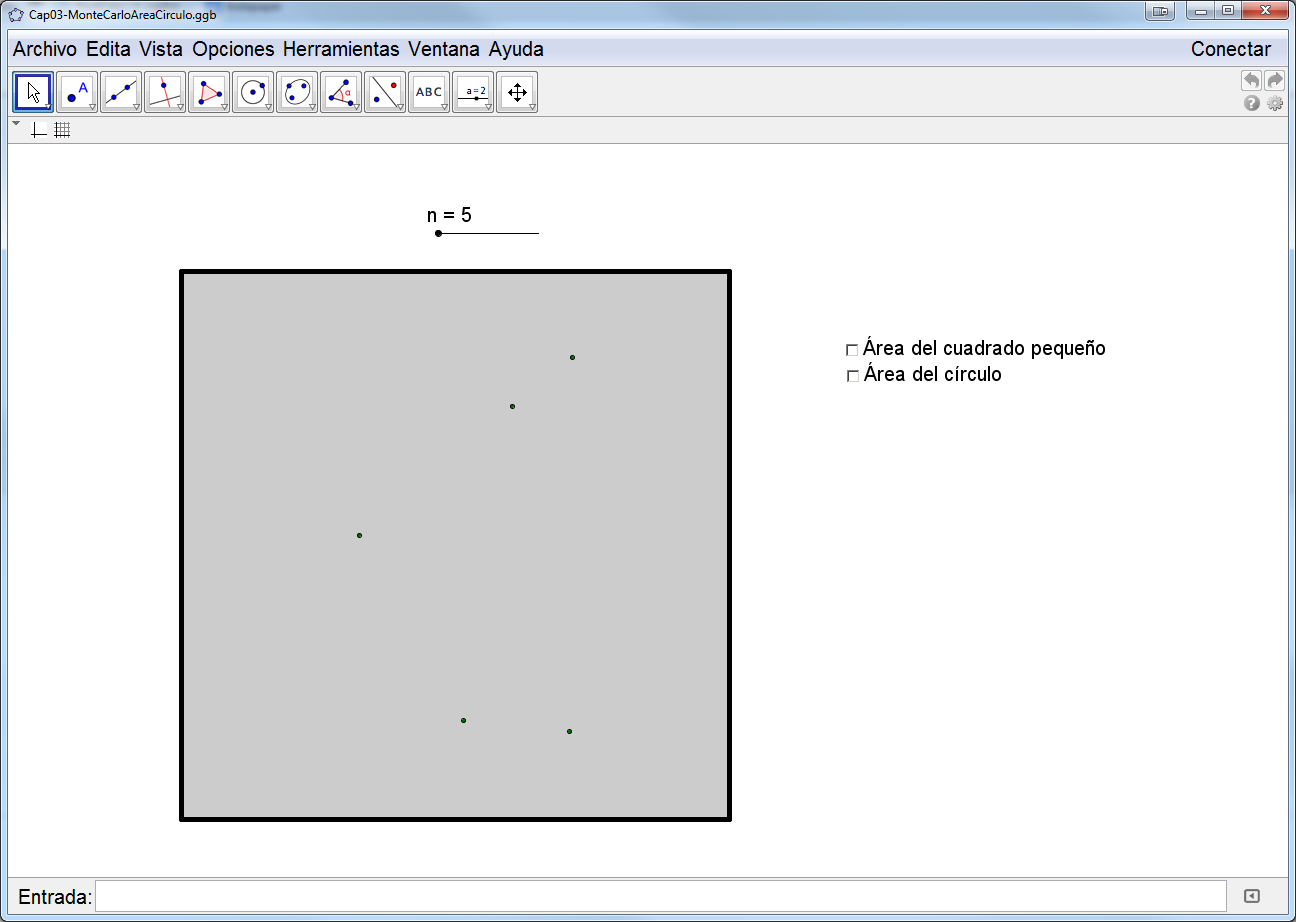
\includegraphics[width=15cm]{./fig/Tut03-43.png}\\[3mm]
(b)\\[3mm]
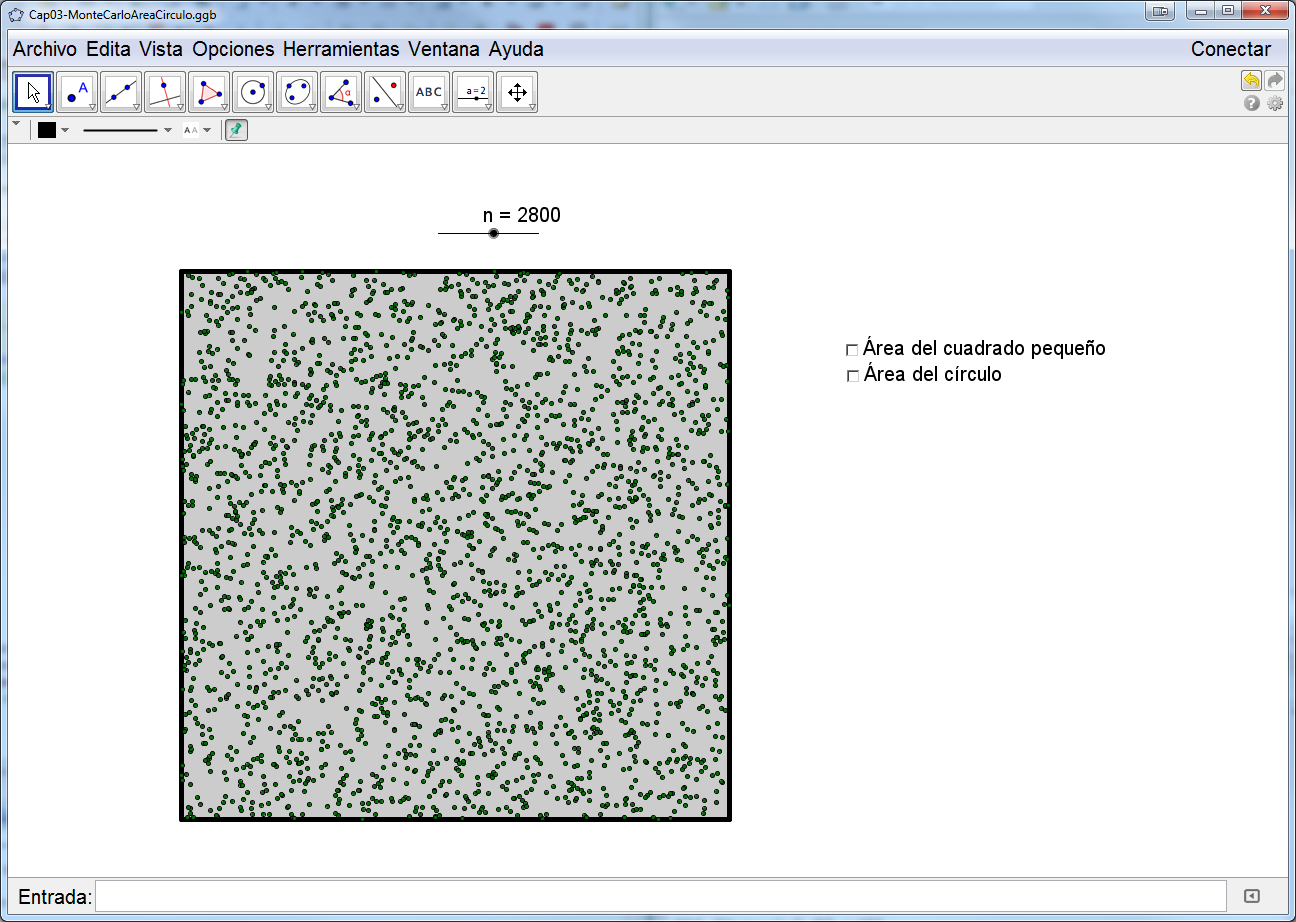
\includegraphics[width=15cm]{./fig/Tut03-44.png}
\end{center}
\caption{(a) Abriendo el fichero {\tt Cap03-MonteCarloAreaCirculo.ggb} con GeoGebra (b) Más puntos al mover el deslizador...}
\label{tut03:fig:MontecarloAreaCirculo01}
\end{figure}
Si ahora marcas con el ratón la casilla rotulada {\em ``Área del cuadrado pequeño''}, verás aparecer un cuadrado más pequeño, de color rojo y centrado en el cuadrado más grande, al que vamos a llamar $C_2$. El lado de este cuadrado más pequeño es $2$, así que su área es $4$. Pero vamos a {\em fingir} que no sabemos cuánto vale el área, y vamos a tratar de calcular ese valor lanzando dardos, y contando la proporción de dardos que hacen blanco en el cuadrado pequeño. La idea subyacente es que ese número de dardos que aciertan en $C_2$ es proporcional al área de $C_2$, así que tenemos:
     \[
          \dfrac{\mbox{Dardos en $C_2$}}{\mbox{Total de dardos (en $C_1$)}} =
               \dfrac{\mbox{Área de $C_2$}}{\mbox{Área de $C_1$}}
          \]
En la Figura \ref{tut03:fig:MontecarloAreaCirculo02} se muestra ese proceso. Puedes ver que hemos lanzado $n=3000$ dardos, y que la proporción de aciertos en $C_2$ es $0.265$. Así que usando la ecuación anterior, y sabiendo que el área de $C_1$ es 16, estimamos que:
     \[
          \mbox{Área de $C_1$} \approx 16\cdot 0.265\approx 4.24
          \]
Que, sin ser impresionante, es una primera aproximación. Prueba a mover el deslizador para ver como,  a medida que el número de puntos aumenta, las estimaciones son cada vez mejores. Puedes moverlos hasta $n=5000$. Y una vez que llegues a ese valor, pulsa {\tt Ctrl + R}. Cada vez que lo hagas, GeoGebra volverá a lanzar $5000$ nuevos dardos, y podrás ver una nueva estimación del área de $C_2$ (también puedes mover el deslizador ligeramente para conseguir lo mismo).

\begin{figure}[htbp]
\begin{center}
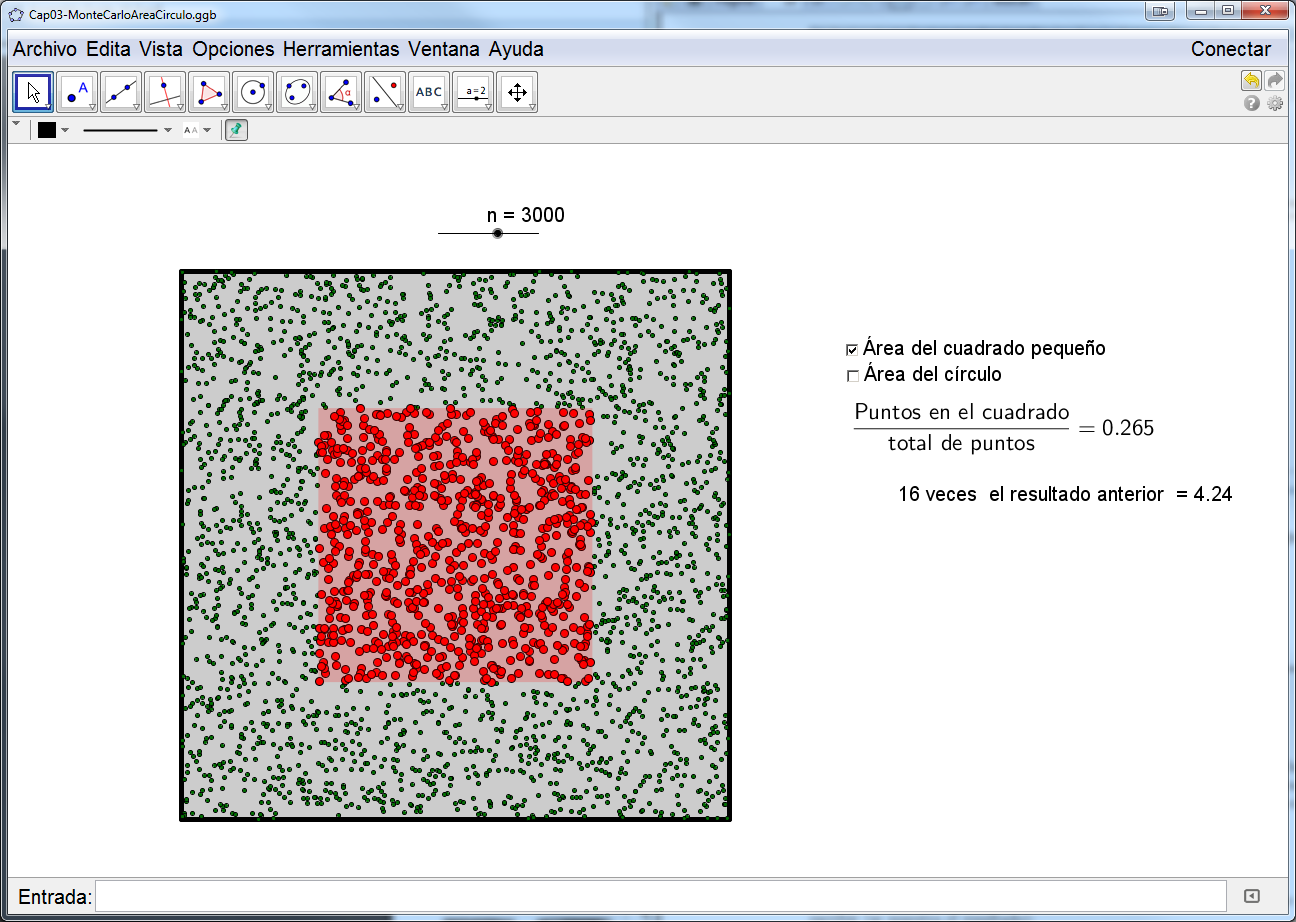
\includegraphics[width=15cm]{./fig/Tut03-45.png}\\[3mm]
\end{center}
\caption{Lanzando dardos para calcular el área del cuadrado pequeño.}
\label{tut03:fig:MontecarloAreaCirculo02}
\end{figure}
Todo eso puede estar muy bien, pero el lector estará pensando que ya sabemos calcular (y de forma exacta) el área de un cuadrado. Al fin y al cabo de ahí hemos sacado el área  $16$ de $C_1$, para empezar. Es cierto. Pero lo interesante empieza ahora, el cuadrado era sólo calentamiento. Desmarca la casilla del cuadrado, y marca la del círculo. Vamos a llamar $C_3$ al círculo que aparece, y cuyo radio es $1$. Imagínate de nuevo que no conocemos la fórmula para el área del círculo.   El razonamiento es el mismo, y nos conduce a la relación:
     \[
          \dfrac{\mbox{Dardos en $C_3$}}{\mbox{Total de dardos (en $C_1$)}} =
               \dfrac{\mbox{Área de $C_3$}}{\mbox{Área de $C_1$ (es 16)}}
          \]
Por lo tanto,
\[
     \mbox{Área de $C_3$}\approx 16\cdot \dfrac{\mbox{Dardos en $C_3$}}{\mbox{Total de dardos (en $C_1$)}}.
     \]
Así que esto nos proporciona un procedimiento para aproximar el área del círculo (o de cualquier otra figura, por cierto) lanzando dardos. Eso empieza a parecer más interesante, ¿verdad?

Vuelve a repetir los pasos que dimos con el cuadrado, moviendo el deslizador hacia la derecha para ver como cambia la aproximación. Y cuando llegues a $5000$ dardos, usa {\tt Ctrl + R} para hacer varios experimentos. Al cabo de unos cuantos intentos espero que te hayas convencido de que el área del círculo tiene un valor cercano a $3.1$. El valor real, naturalmente, es $\pi$. Así que es posible calcular el valor de $\pi$ mientras juegas a los dardos (como ilustra la Figura \ref{tut03:fig:MontecarloAreaCirculo03})... siempre que estés dispuesto a jugar durante un buen rato, y no te esfuerces lo más mínimo en apuntar.
\begin{figure}[h!]
\begin{center}
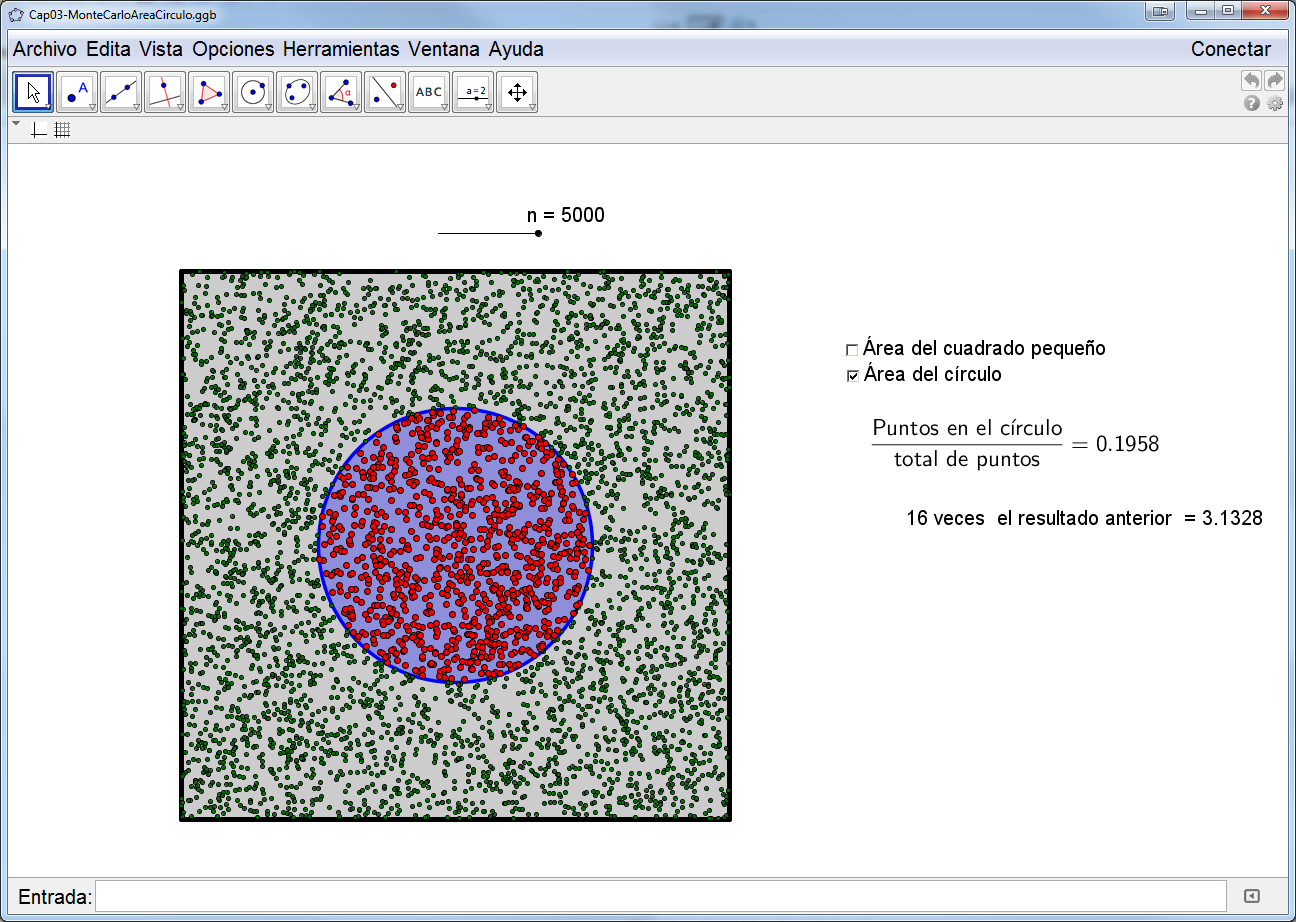
\includegraphics[width=15cm]{./fig/Tut03-45a.png}\\[3mm]
\end{center}
\caption{Lanzando dardos para calcular el área del círculo, que es precisamente $\pi$.}
\label{tut03:fig:MontecarloAreaCirculo03}
\end{figure}
Recuerda que lo esencial de estos experimentos es observar el vínculo que existe entre áreas y probabilidades. Cuanto mayor es el área de una figura, mayor es la probabilidad de acertarle con un dardo lanzado al azar.


\section{Operaciones simbólicas. Wiris, Wolfram Alpha.}
\label{tut03:sec:OperacionesSimbolicas}

Cuando empezamos a trabajar con probabilidades, usando al principio la Regla de Laplace, y luego con la Combinatoria, a menudo nos surge la necesidad de operar con fracciones,  como en el cálculo de esta fracción (que procede del Ejemplo \ref{curso-cap03:ejem:EjemploUrnasBayes}, pág. \pageref{curso-cap03:ejem:EjemploUrnasBayes}, de nuestro curso):
     \[
          \dfrac{\dfrac{3}{5}\cdot \dfrac{2}{6}}{\dfrac{3}{5}\cdot \dfrac{2}{6}+\dfrac{4}{5}\cdot\dfrac{4}{6}}=\dfrac{3}{11}
          \]
Si intentas hacer esta cuenta en R, para empezar tienes que ser cuidadoso con los paréntesis (se aplica la regla de ``más vale que sobren''), y escribir:
\begin{knitrout}
\definecolor{shadecolor}{rgb}{0.969, 0.969, 0.969}\color{fgcolor}\begin{kframe}
\begin{alltt}
\hlstd{( (}\hlnum{3}\hlopt{/}\hlnum{5}\hlstd{)} \hlopt{*} \hlstd{(}\hlnum{2}\hlopt{/}\hlnum{6}\hlstd{) )} \hlopt{/}\hlstd{( (}\hlnum{3}\hlopt{/}\hlnum{5}\hlstd{)} \hlopt{*} \hlstd{(}\hlnum{2}\hlopt{/}\hlnum{6}\hlstd{)} \hlopt{+} \hlstd{(}\hlnum{4}\hlopt{/}\hlnum{5}\hlstd{)} \hlopt{*} \hlstd{(}\hlnum{4}\hlopt{/}\hlnum{6}\hlstd{) )}
\end{alltt}
\begin{verbatim}
## [1] 0.273
\end{verbatim}
\end{kframe}
\end{knitrout}
     Fíjate en los espacios que hemos dejado para hacer la expresión más legible. La respuesta
0.273
no es exactamente lo que queríamos. Para un problema como este, es muy posible que queramos ver el resultado en forma de fracción. El problema es que R es un programa esencialmente {\sf numérico}, que trabaja con la representación de los números en forma decimal (podemos {\em obligarle}, hasta cierto punto, a trabajar con fracciones, pero no es su lenguaje natural). Mientras que 0.273 es una versión {\sf numérica} de la respuesta, en el sentido de {\em redondeada a unas cuantas cifras significativas} y, por lo tanto, es una respuesta aproximada. En cambio la respuesta en forma de fracción
\[
     \dfrac{3}{11}
     \]
es una respuesta {\sf simbólica}, y es absolutamente exacta: no hay ninguna pérdida de precisión. Usamos la dualidad {\em numerico/simbólico} en el sentido habitual en las matemáticas contemporáneas. En ese sentido, las cantidades
\[\sqrt{2},\qquad \pi\]
son cantidades simbólicas, mientras que sus contrapartes numéricas (con cinco cifras significativas) son:
     \[1.4142,\qquad 3.1416\]
Y conviene insistir en que R es un programa numérico, no simbólico. Por eso, para algunas operaciones del curso vamos a tener que recurrir a la ayuda de programas simbólicos. Veamos algunos.

\subsection{Wiris.}
\label{tut03:subsec:Wiris}

El programa Wiris CAS (de Computer Algebra System) es una creación de la empresa de software matemático {\em Maths for More}, con sede en Barcelona, y fundada por profesores y antiguos estudiantes de la Universitat Politècnica de Catalunya. Para utilizar el programa debemos estar conectados a internet.  El programa se usa en el navegador, a través de la Web, en la página de la propia empresa (que incluye publicidad insertada en la página):
     \begin{center}
\link{http://www.wiris.net/demo/wiris/es/index.html}{http://www.wiris.net/demo/wiris/es/index.html}
\end{center}
o a través de las páginas Wiris que algunas Consejerías de Educación de distintas comunidades autónomas españolas ponen a libre disposición del público (tras llegar a acuerdos con la empresa, claro). Aquí tienes, por ejemplo, el enlace de la Comunidad de Madrid:
     \begin{center}
\link{http://www.wiris.net/educa.madrid.org/wiris/es/index.html}{http://www.wiris.net/educa.madrid.org/wiris/es/index.html}
\end{center}
Usemos esta última. Al abrirla (es necesario tener instalado \link{http://www.java.com/es/download/}{Java} en el ordenador; si no sabes si lo tienes, o si puedes o debes instalarlo, consulta a un \ninja{ninja informático),} el aspecto es este:
     \begin{center}
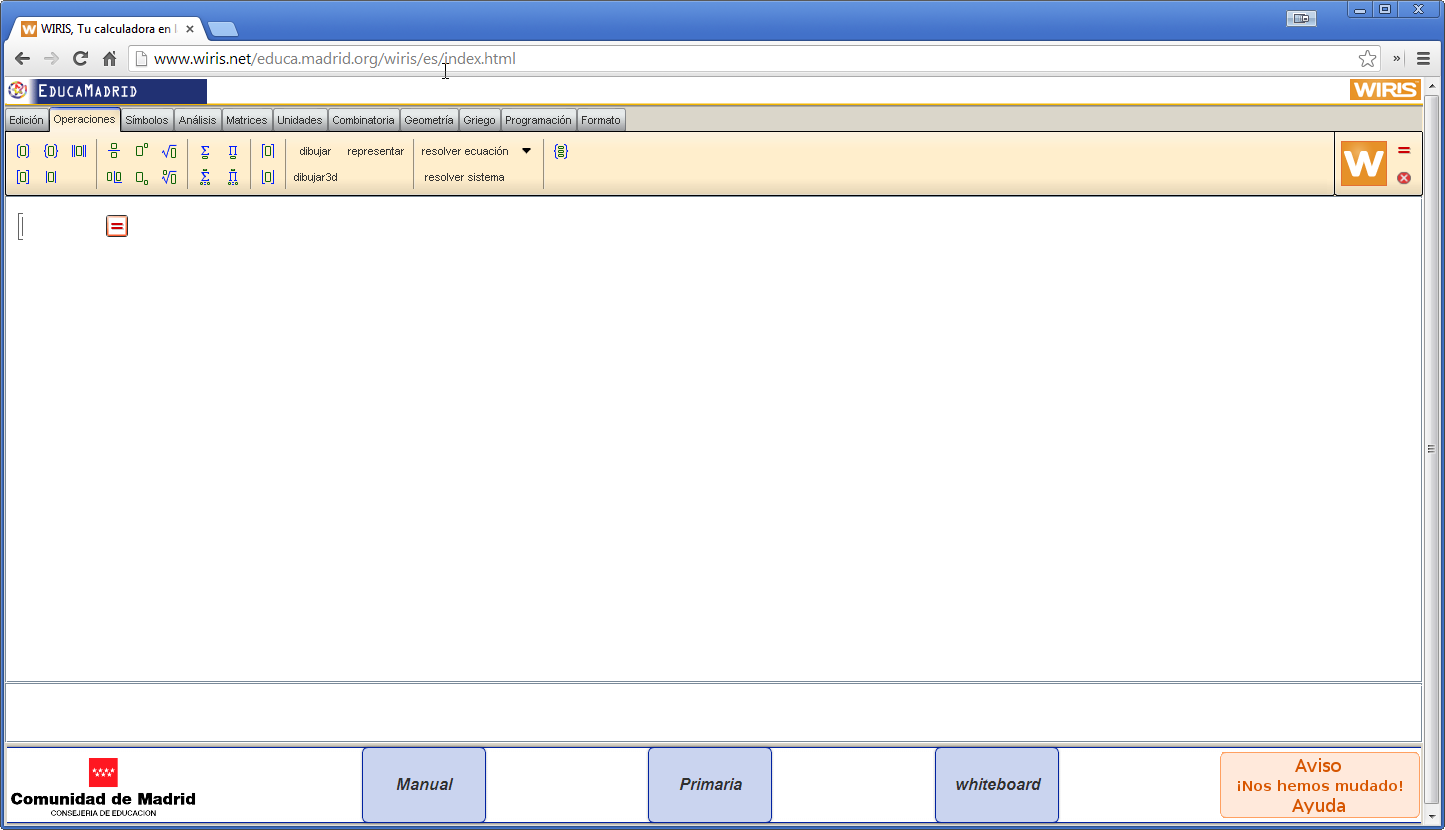
\includegraphics[width=15.5cm]{./fig/Tut04-09.png}
\end{center}
Wiris CAS nos permite escribir fórmulas matemáticas usando una notación muy parecida a la que usaríamos en el papel o la pizarra. Los símbolos y operaciones matemáticas están organizados por pestañas, pero para este primer ejemplo tan sencillo, todo lo que necesitamos está en la pestaña operaciones. Busca en ella el símbolo de fracción, que es el icono:
     \begin{center}
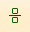
\includegraphics[width=1cm]{./fig/Tut04-10.png}
\end{center}
Púlsalo una vez con el ratón, y obtendrás
\begin{center}
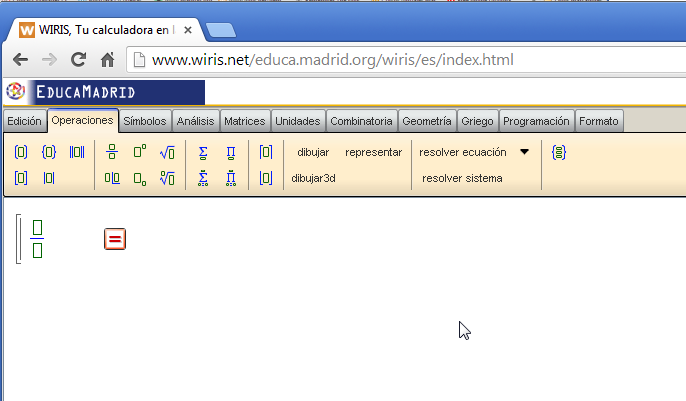
\includegraphics[width=15cm]{./fig/Tut04-11.png}
\end{center}
A partir de aquí las cosas son bastante intuitivas. Tienes que usar las teclas {\tt +} para la suma, y {\tt *} para la multiplicación, y usar el icono de fracción cada vez que quieras crear una nueva fracción. Tus primeros pasos te pueden llevar a algo como esto:
     \begin{center}
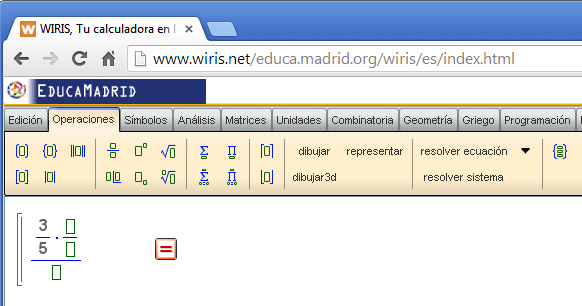
\includegraphics[width=15.5cm]{./fig/Tut04-12.png}
\end{center}
Ten en cuenta, para avanzar más rápido, que puedes seleccionar trozos de la fórmula con el ratón, y copiarlos y pegarlos. También, que en la pestaña {\tt Edición} tienes dos iconos en forma de flechas curvas, para deshacer y rehacer operaciones. Debes llegar a:
     \begin{center}
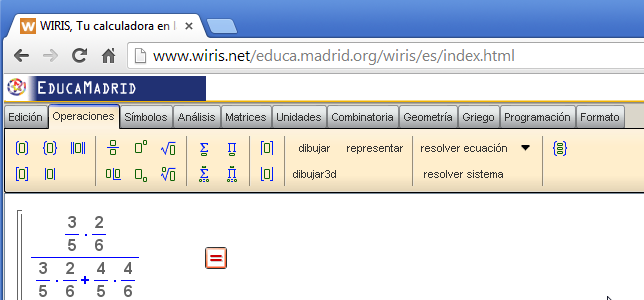
\includegraphics[width=15.5cm]{./fig/Tut04-13.png}
\end{center}
Y ahora viene lo bueno. Una vez que estés ahí, pulsa sobre el icono {\em igual} que hay a la derecha de la fórmula (o, con el cursor situado en la fórmula, pulsa {\tt Ctrl+Enter}). Al cabo de unos instantes (tu fórmula viaja por la red, se calcula, y la respuesta vuela de vuelta a tu ordenador), tendrás la respuesta:
     \begin{center}
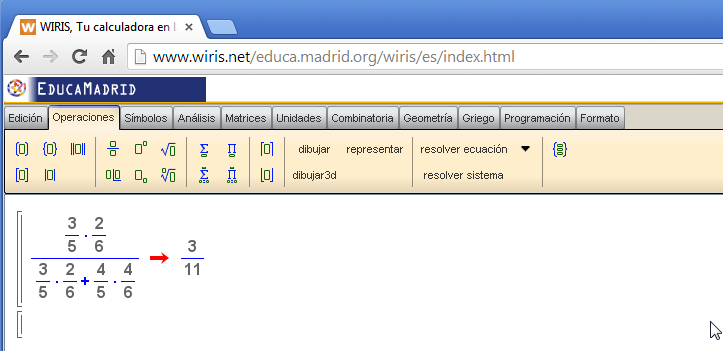
\includegraphics[width=15.5cm]{./fig/Tut04-14.png}
\end{center}
Y Wiris CAS está listo para nuestra siguiente pregunta. Como ves, la respuesta es simbólica, no numérica, como queríamos. El inconveniente que encontramos es que la respuesta es realmente una imagen en la pantalla, no un número que podamos cortar y pegar para llevar a otro programa.

El cálculo de este ejemplo ha sido muy sencillo, pero a lo largo del curso iremos viendo más ejemplos en los que Wiris CAS nos puede ser de gran ayuda.

\subsection{Wolfram Alpha.}
\label{tut03:subsec:WolframAlpha}

Se trata también de una herramienta sólo accesible a través de la Web, en este caso en inglés, pero que también es muy interesante (por ejemplo, es fácilmente accesible desde teléfonos móviles o tablets). Al abrir la dirección
\begin{center}
\link{http://www.wolframalpha.com/}{http://www.wolframalpha.com/}
\end{center}
Wolfram Alpha te recibe con una pantalla como esta:
     \begin{center}
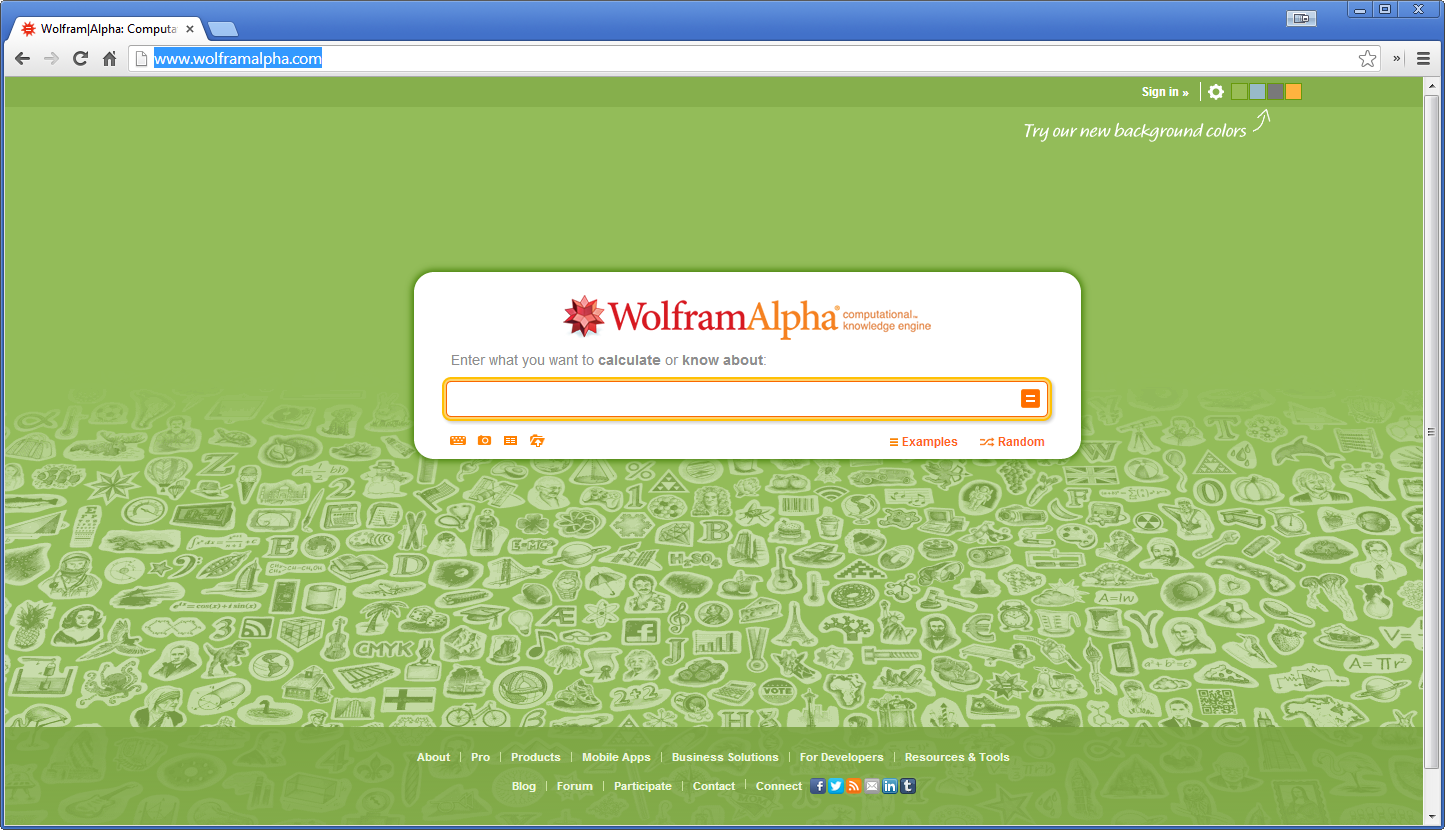
\includegraphics[width=15.5cm]{./fig/Tut04-15.png}
\end{center}
Debemos introducir lo que queremos calcular en el campo de entrada del centro de la ventana, usando en este caso la misma sintaxis que en R:
     \begin{center}
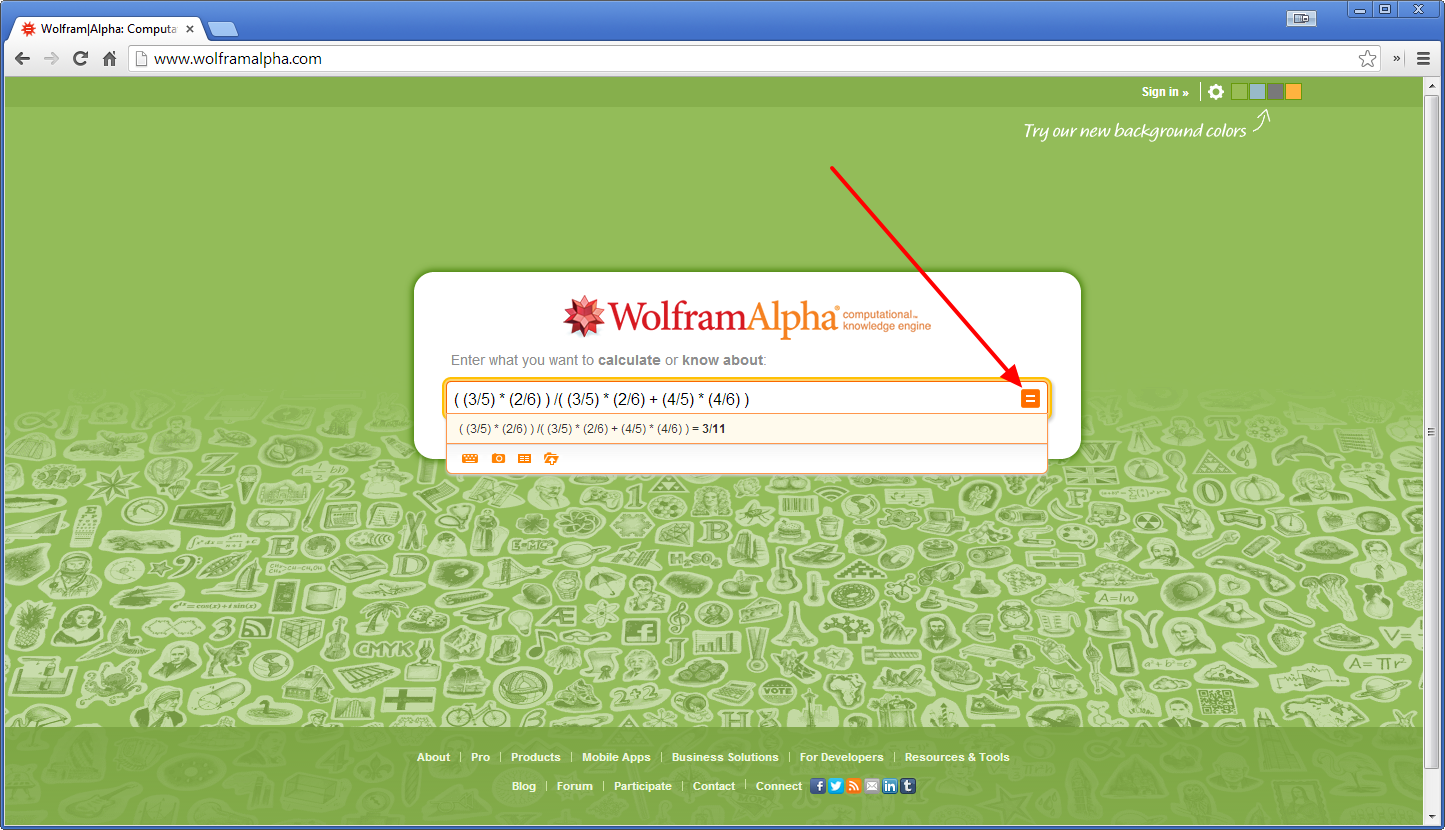
\includegraphics[width=15.5cm]{./fig/Tut04-16.png}
\end{center}
En este caso, como ves, en cuanto hemos tecleado la operación, Wolfram Alpha nos ha mostrado la respuesta. Pero para hacer el ejemplo más completo, pulsa sobre el símbolo igual que hay al final del campo de entrada. Verás una pantalla parecida a esta,
\begin{center}
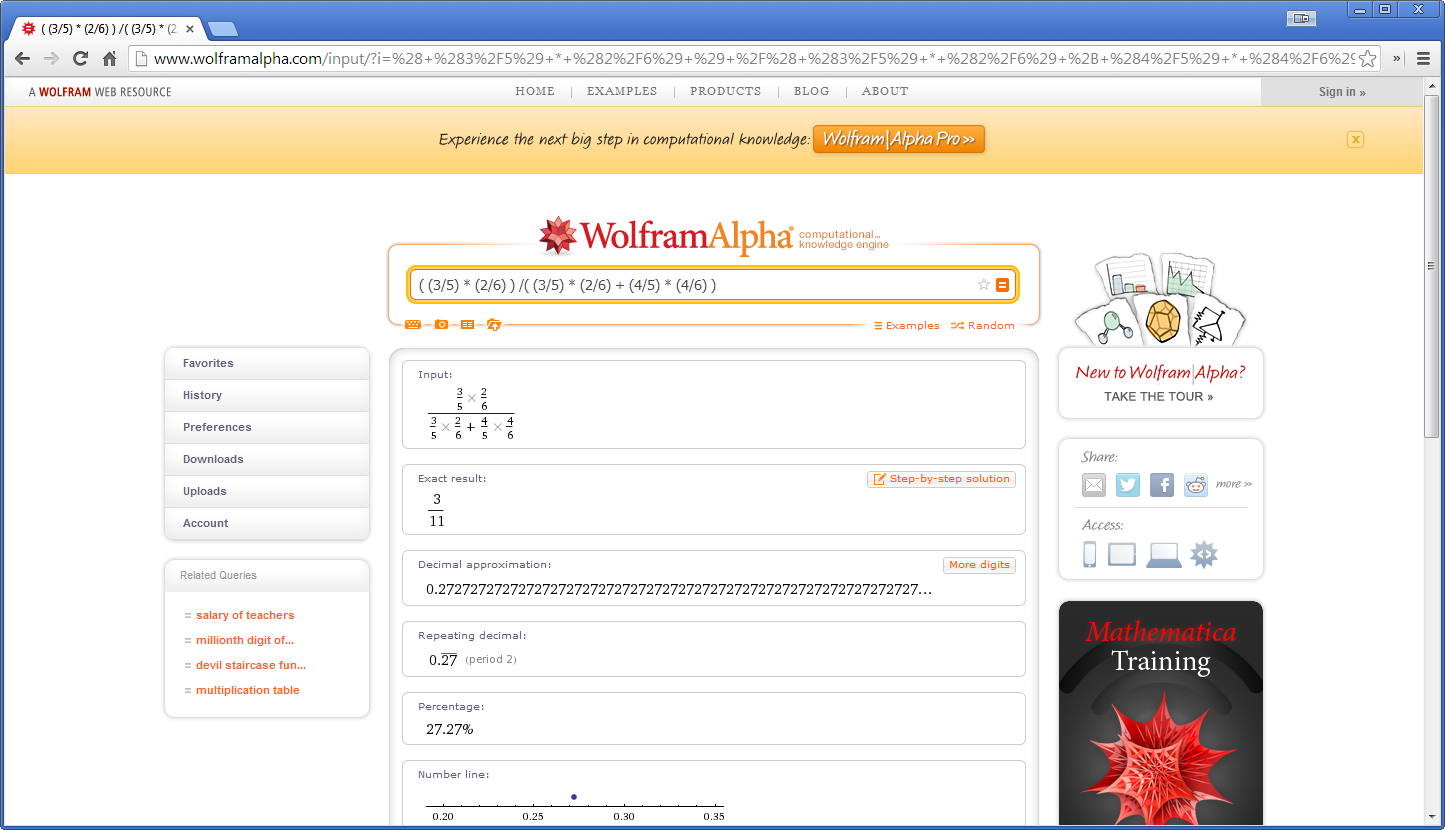
\includegraphics[width=15.5cm]{./fig/Tut04-17.png}
\end{center}
en la que, desde luego, está la respuesta a tu pregunta, pero que contiene además mucha más información matemática sobre esa pregunta (más de la que seguramente nunca pensaste que existiera...) Como en el caso de Wiris CAS, apenas hemos rozado la superficie de lo que Wolfram Alpha es capaz de hacer, y volveremos más adelante a seguir aprendiendo como usarlo. Si quieres, puedes pulsar en el enlace {\tt Examples} que aparece bajo la barra de entrada para ver algunas de esas cosas.


\subsection{Suma de series con Wiris y Wolfram Alpha.}
\label{tut05:subsec:SeriesWirisWolfram}

Una serie es una suma con infinitos sumandos, como la suma
\[\dfrac{1}{2}+\dfrac{1}{2^3}+\dfrac{1}{2^5}+\dfrac{1}{2^7}+\cdots=\dfrac{2}{3}.\]
que vimos en el Ejemplo \ref{curso-cap03:ejem:LanzamientoMonedaHastPrimeraCara:2} (pág. \pageref{curso-cap03:ejem:LanzamientoMonedaHastPrimeraCara:2}) del libro. La teoría matemática de este tipo de sumas puede llegar a ser muy complicada. Pero nosotros nos vamos a quedar en la superficie, limitándonos a usar el ordenador para calcular los ejemplos que necesitemos.

El primer ejemplo, el más sencillo de todos, nos permite comprobar que la probabilidad total asignada en ese Ejemplo \ref{curso-cap03:ejem:LanzamientoMonedaHastPrimeraCara:2} es igual a 1, como exigen las propiedades básicas de la Probabilidad. Es decir, que queremos ver que:
     \[ \dfrac{1}{2}+\dfrac{1}{2^2}+\dfrac{1}{2^3}+\dfrac{1}{2^4}+\cdots=1. \]
En la primera suma de esta sección sumábamos sólo los términos con exponentes impares, aquí los sumamos todos. Para calcular esta suma usaremos Wiris. Una vez abierto, en la pestaña {\tt Operaciones}, busca el icono del sumatorio
\begin{center}
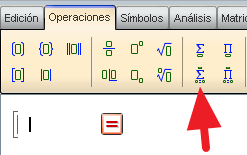
\includegraphics[width=6.5cm]{./fig/Tut05-02.png}
\end{center}
Y usa la paleta de símbolos de esa misma pestaña para escribir la serie, como en la siguiente figura. Un par de advertencias:
     \begin{itemize}
\item Encontrarás el símbolo de infinito positivo ($+\infty$) en la pestaña {\tt Símbolos}.
\item Para escribir un exponente en Wiris puedes, desde luego, usar el botón 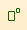
\includegraphics[width=0.3cm]{./fig/Tut05-03.png} de la pestaña {\tt Operaciones}. Pero es más rápido usar el atajo de teclado {\tt Ctrl+$\uparrow$}.
\end{itemize}
\begin{center}
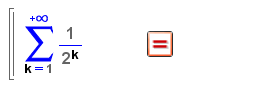
\includegraphics[width=5cm]{./fig/Tut05-04.png}
\end{center}
Pulsa sobre el símbolo igual, y verás como Wiris te confirma que el resultado de sumar esa serie es un 1.

Ahora vamos a modificar ligeramente este cálculo, para obtener la suma de la serie de los términos con exponentes impares con la que empezamos esta sección. Para conseguir esto, vamos a modificar el exponente para que sólo tome valores impares. La forma de conseguirlo es sustituir, en el exponente, la variable $k$ por la fórmula $2\cdot k-1$. Porque, cuando $k$ recorre los valores $1,2,3,\ldots$, la fórmula $2\cdot k-1$ recorre a su vez los valores impares $1,3,5,\ldots$
     
     Por lo tanto, hacemos ese cambio en Wiris, volvemos a pulsar el símbolo igual y obtenemos el resultado que se muestra en esta figura:
     \begin{center}
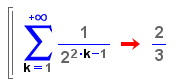
\includegraphics[width=5cm]{./fig/Tut05-05.png}
\end{center}

Como hemos dicho, las matemáticas de las series pueden ser muy complicadas. Queremos, para cerrar esta brevísima visita, añadir un ejemplo final, que ilustra un punto importante de esa teoría. La suma de esta serie
\[1+\dfrac{1}{2}+\dfrac{1}{3}+\cdots+\dfrac{1}{n}+\cdots\]
es infinito. Si le preguntas a Wiris, en este caso protestará, y dirá que no ha sido capaz de calcularlo (mira en la parte inferior de la pantalla). Lo malo es que a veces obtendremos esa misma respuesta con series que son ``demasiado complicadas para Wiris'', pero cuya suma es una cantidad finita. Si alguna vez necesitas necesitas más detalles, puedes consultar el
\link{http://www.wiris.net/educa.madrid.org/wiris/manual/es/html/tour/analisi.html\#series}{manual de Wiris } al respecto.
      
      También  puedes probar con Wolfram Alpha. Ya sabes, la dirección es
      
      \begin{center}
      \link{http://www.wolframalpha.com/}{http://www.wolframalpha.com/}
      \end{center}
      
      Prueba a escribir en el campo de entrada
      \begin{center}
      \begin{minipage}{12cm}
      sum (1/n)
      \end{minipage}
      \end{center}
      
      y obtendrás esta respuesta
      \begin{center}
      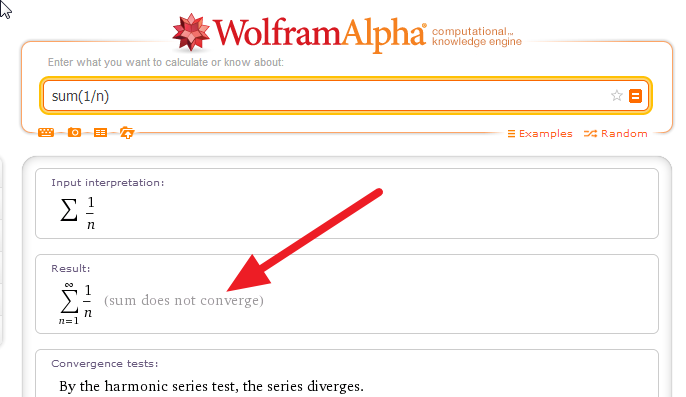
\includegraphics[width=8cm]{./fig/Tut05-06.png}
      \end{center}
      La frase {\tt sum does not converge} (la suma --o serie-- no converge) se debe, en este caso, a que el resultado no es un número finito\footnote{Aparte de que el resultado sea infinito,  pueden ocurrir otras cosas. La serie converge cuando el resultado es un número finito, y no converge en cualquier otro caso.}
      
      ¿Por qué esta suma es infinito, mientras que las anteriores daban resultados finitos? La respuesta es que una serie es una suma de infinitos números,
      cada vez más pequeños, y que el factor clave para que la suma sea finita es la {\em velocidad} a la que los números se hacen pequeños. Si se hacen
      pequeños muy rápido,  la serie tendrá una suma finita (el resultado de la suma dependerá de cómo sea esa velocidad, en detalle). Pero si los números,
      por el contrario, aunque se hagan pequeños, lo hacen despacio, entonces la suma se irá haciendo cada vez más grande, hasta valer infinito, {\em en el límite}.
      
      
      \section{Combinatoria en R. Cómo instalar librerías adicionales.}
      \label{tut03:sec:CombinatoriaR}
      
      R proporciona algunas herramientas básicas para hacer cálculos en Combinatoria. Para empezar, la función {\tt factorial}, que se usa como muestra este ejemplo de código:
\begin{knitrout}
\definecolor{shadecolor}{rgb}{0.969, 0.969, 0.969}\color{fgcolor}\begin{kframe}
\begin{alltt}
\hlkwd{factorial}\hlstd{(}\hlnum{6}\hlstd{)}
\end{alltt}
\begin{verbatim}
## [1] 720
\end{verbatim}
\end{kframe}
\end{knitrout}
           El factorial de $n$, {\tt fact(n)} en el lenguaje de R, da como resultado el producto de todos los elementos que forman el vector {\tt 1:n}. Y no es de extrañar que en R exista una función {\tt prod}, para multiplicar todos los elementos de un vector:
\begin{knitrout}
\definecolor{shadecolor}{rgb}{0.969, 0.969, 0.969}\color{fgcolor}\begin{kframe}
\begin{alltt}
\hlkwd{prod}\hlstd{(}\hlnum{1}\hlopt{:}\hlnum{6}\hlstd{)}
\end{alltt}
\begin{verbatim}
## [1] 720
\end{verbatim}
\end{kframe}
\end{knitrout}
           La ventaja de {\tt prod} frente a {\tt fact} es, desde luego, que los elementos no tienen porque ser naturales, ni consecutivos, etc. Puesto que casi todos los cálculos de Combinatoria que vamos a usar en el curso se basan en el factorial, podríamos parar aquí. Pero el factorial es una forma extremadamente poco eficiente de hacer cálculos. Para trabajar de una forma más sensata, por ejemplo, al calcular números combinatorios, R nos ofrece la función {\tt choose}. La forma de utilizar esta función para  calcular el número combinatorio
      \[\binom{22}{7}\]
      es esta:
\begin{knitrout}
\definecolor{shadecolor}{rgb}{0.969, 0.969, 0.969}\color{fgcolor}\begin{kframe}
\begin{alltt}
\hlkwd{choose}\hlstd{(}\hlkwc{n}\hlstd{=}\hlnum{22}\hlstd{,}\hlkwc{k}\hlstd{=}\hlnum{7}\hlstd{)}
\end{alltt}
\begin{verbatim}
## [1] 170544
\end{verbatim}
\end{kframe}
\end{knitrout}
           
           \subsection{Librerías adicionales en R.}
      \label{tut03:subsec:LibreriasAdicionalesR}
      
      Con estas dos herramientas podemos resolver la mayoría de las preguntas que surgen en los problemas elementales de Probabilidad, al aplicar la Regla de Laplace, cuando queremos calcular el {\em número} de casos posibles o de casos favorables a un suceso. Pero no nos sirven si lo que queremos es, de hecho, enumerar esos casos y construir realmente la lista completa de casos.
      
      Por ejemplo, en el caso que usamos muchas veces de las tiradas de un par de dados. Sabemos por un lado que hay 36 resultados posibles distintos. Pero si queremos obtener la lista, entonces queremos obtener los resultados en una forma similar a
      \[(1,1) , (1,2), \ldots, (4,3), \ldots,(6,5), (6,6).\]
      Hasta ahora nos hemos limitado a representar los resultados de las dos tiradas mediante números del $1$ al $36$. Pero  esa representación no es siempre conveniente y, en problemas más complicados, las representaciones análogas, que nos alejan de la estructura real de los datos, se convierten en un inconveniente cada vez mayor. Así que nos conviene buscar maneras de representar los datos en R tal y como son, de la manera más fidedigna posible.
      
      Vamos a utilizar este problema para aprender algunas cosas más sobre R. La instalación de R, tal como hemos aprendido a hacerla en el Tutorial02, incluye sólo una pequeña parte de todo lo que es posible hacer con R. Porque una de las ventajas que se desprenden del hecho de que R sea un programa de código abierto es la gran cantidad de paquetes de código R que se han escrito, para resolver los problemas más variados. Ya hemos visto cómo guardar nuestros propios fragmentos de código en R. Otros usuarios, a menudo expertos en R y en alguna de sus aplicaciones, escriben sus propios fragmentos de código, a veces muy sofisticados, para resolver problemas. Y después ponen esos fragmentos de código, llamados a veces paquetes o librerías,  a disposición de la comunidad de usuarios de R, de forma libre y gratuita. A fecha de hoy, R-cran, que es el mayor almacén de código R, contiene más de 5600 de esos paquetes (y la cifra aumenta constantemente).
      
      Cuando instalas  R en tu ordenador, normalmente sólo instalas una pequeña parte de esos paquetes, para no hacer la instalación innecesariamente larga y complicada. En RStudio, el panel inferior izquierdo contiene una pestaña llamada {\tt Packages}, en la que puedes ver la lista de las librerías que actualmente tienes instaladas. Tu lista será, muy probablemente, diferente de la mía (y, si tienes una versión reciente de RStudio, incluirá una pestaña adicional, llamada {\tt Viewer}).
      \begin{center}
      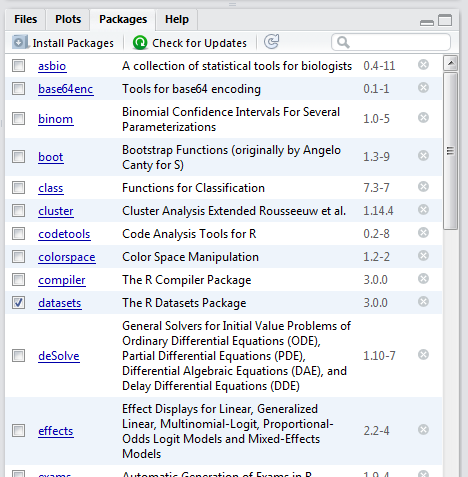
\includegraphics[width=6cm]{./fig/Tut05-10.png}
      \end{center}
      Si en algún momento necesitas uno de los paquetes  que no has instalado, puedes conectar con un almacén de paquetes en Internet, descargarlo e instalarlo de forma casi automática. Para ello, asegúrate de que tu ordenador está conectado a la red. Si es así, en RStudio basta con que pulses sobre el botón {\tt Install Packages} de esa ventana, y que teclees el nombre del paquete en el campo {\tt Packages} de la ventana que se abre (ver la siguiente figura).
      
      Para practicar esto y, de paso, mejorar las habilidades Combinatorias de R vamos a instalar un paquete llamado {\tt gtools}. Así que escribe ese nombre en el campo {\em packages} (a medida que escribes el nombre, verás que RStudio lo reconoce como uno de los  paquetes disponibles).
      \begin{center}
      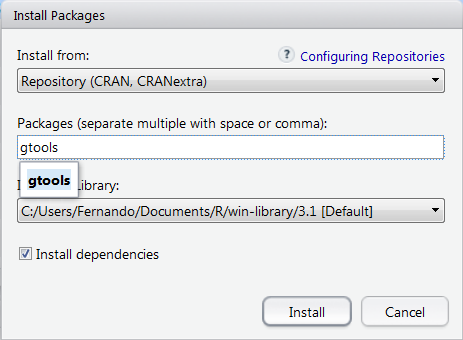
\includegraphics[width=7cm]{./fig/Tut03-InstalarGtools2.png}
      \end{center}
      Después pulsa sobre el botón {\tt Install}, y verás como R realiza una serie de operaciones (descarga e instalación, básicamente). Si, por alguna razón, no usas RStudio, siempre puedes ejecutar este comando en la consola de R:
\begin{knitrout}
\definecolor{shadecolor}{rgb}{0.969, 0.969, 0.969}\color{fgcolor}\begin{kframe}
\begin{alltt}
\hlkwd{install.packages}\hlstd{(}\hlkwc{pkgs}\hlstd{=}\hlstr{"gtools"}\hlstd{,}\hlkwc{dependencies}\hlstd{=}\hlnum{TRUE}\hlstd{)}
\end{alltt}
\end{kframe}
\end{knitrout}
           Ya hemos instalado el paquete {\tt gtools}, pero todavía falta un paso más. De la misma forma que la instalación de R no incluye todos los paquetes que existen (más de $5600$, sólo en CRAN), es posible que al cabo de un tiempo tengas instalados en tu ordenador decenas o cientos de paquetes. Y no queremos sobrecargar la memoria del ordenador, haciéndole cargar todos esos paquetes en cada sesión de trabajo (además, algunos de ellos podrían interferir entre sí). Por esa razón, cada vez que vayamos a usarlo tenemos que decirle a R que, para nuestro trabajo en esa sesión, queremos usar ese paquete en concreto. La forma de decirle a R que quiero usar ese paquete es mediante el comando:
\begin{knitrout}
\definecolor{shadecolor}{rgb}{0.969, 0.969, 0.969}\color{fgcolor}\begin{kframe}
\begin{alltt}
\hlkwd{library}\hlstd{(}\hlstr{"gtools"}\hlstd{)}
\end{alltt}
\end{kframe}
\end{knitrout}
           Al ejecutarlo puede que aparezca alguna advertencia ({\tt warning}) de R sobre el número de versión. No te preocupes, mientras no aparezcan mensajes de error. Tras la instalación, ya podemos empezar el trabajo de Combinatoria con R.
      
      \subsection{Lista de Permutaciones y combinaciones con R.}
      \label{tut03:subsec:PermutacionesCombinacionesR}
      
      El paquete {\tt gtools} añade (entre otras muchas cosas) dos funciones nuevas a R, {\tt permutations} y {\tt combinations}, que nos van a servir precisamente para obtener esos resultados. En España, como hemos visto en el curso, distinguimos entre variaciones y permutaciones, pero la tradición anglosajona engloba dentro del término {\em permutations} tanto las variaciones como las permutaciones.
      
      Insistimos en que no se trata de saber cuántos hay, sino, de hecho, de construirlos y enumerarlos. Para ver en acción a estas funciones de R, vamos a utilizarlas para fabricar todas las listas posibles de tres elementos, elegidos de entre cuatro posibles. Para empezar, no admitimos repeticiones de los elementos. Entonces, si el orden no importa, estamos formando las combinaciones de cuatro elementos tomados de tres en tres. Y si el orden importa, entonces se trata de las variaciones (un inglés diría permutaciones) de cuatro elementos tomados de tres en tres.
      
      Los correspondientes comandos son estos (recuerda que has debido ejecutar primero {\tt library("gtools")}). Para las combinaciones:
\begin{knitrout}
\definecolor{shadecolor}{rgb}{0.969, 0.969, 0.969}\color{fgcolor}\begin{kframe}
\begin{alltt}
\hlkwd{combinations}\hlstd{(}\hlnum{4}\hlstd{,}\hlnum{3}\hlstd{)}
\end{alltt}
\begin{verbatim}
##      [,1] [,2] [,3]
## [1,]    1    2    3
## [2,]    1    2    4
## [3,]    1    3    4
## [4,]    2    3    4
\end{verbatim}
\end{kframe}
\end{knitrout}
           Cada fila de la salida contiene una de las combinaciones que buscábamos. Y para las permutaciones:
\begin{knitrout}
\definecolor{shadecolor}{rgb}{0.969, 0.969, 0.969}\color{fgcolor}\begin{kframe}
\begin{alltt}
\hlkwd{permutations}\hlstd{(}\hlnum{4}\hlstd{,}\hlnum{3}\hlstd{)}
\end{alltt}
\begin{verbatim}
##       [,1] [,2] [,3]
##  [1,]    1    2    3
##  [2,]    1    2    4
##  [3,]    1    3    2
##  [4,]    1    3    4
##  [5,]    1    4    2
##  [6,]    1    4    3
##  [7,]    2    1    3
##  [8,]    2    1    4
##  [9,]    2    3    1
## [10,]    2    3    4
## [11,]    2    4    1
## [12,]    2    4    3
## [13,]    3    1    2
## [14,]    3    1    4
## [15,]    3    2    1
## [16,]    3    2    4
## [17,]    3    4    1
## [18,]    3    4    2
## [19,]    4    1    2
## [20,]    4    1    3
## [21,]    4    2    1
## [22,]    4    2    3
## [23,]    4    3    1
## [24,]    4    3    2
\end{verbatim}
\end{kframe}
\end{knitrout}
           \begin{ejercicio}
      \label{tut03:ejercicio13}
      \quad
      Hemos visto ya que en R hay muchos tipos de objetos distintos (vectores, matrices, tablas, etc.) ¿Qué tipo de objetos son los que estamos obteniendo? Solución en la página \pageref{tut03:ejercicio13:sol}.
      \qed
      \end{ejercicio}
      ¿Cómo se usa esto para las tiradas de dos dados? Bueno, si queremos obtener resultados equiprobables, debemos distinguir el orden (como si cada dado fuera de un color) y, además, a diferencia de los dos ejemplos anteriores, debemos permitir resultados repetidos. Con esas premisas, hacemos
{\small
\begin{knitrout}
\definecolor{shadecolor}{rgb}{0.969, 0.969, 0.969}\color{fgcolor}\begin{kframe}
\begin{alltt}
     \hlstd{(dosDados}\hlkwb{=}\hlkwd{permutations}\hlstd{(}\hlnum{6}\hlstd{,}\hlnum{2}\hlstd{,}\hlkwc{repeats.allowed}\hlstd{=}\hlnum{TRUE}\hlstd{))}
\end{alltt}
\begin{verbatim}
##       [,1] [,2]
##  [1,]    1    1
##  [2,]    1    2
##  [3,]    1    3
##  [4,]    1    4
##  [5,]    1    5
##  [6,]    1    6
##  [7,]    2    1
##  [8,]    2    2
##  [9,]    2    3
## [10,]    2    4
## [11,]    2    5
## [12,]    2    6
## [13,]    3    1
## [14,]    3    2
## [15,]    3    3
## [16,]    3    4
## [17,]    3    5
## [18,]    3    6
## [19,]    4    1
## [20,]    4    2
## [21,]    4    3
## [22,]    4    4
## [23,]    4    5
## [24,]    4    6
## [25,]    5    1
## [26,]    5    2
## [27,]    5    3
## [28,]    5    4
## [29,]    5    5
## [30,]    5    6
## [31,]    6    1
## [32,]    6    2
## [33,]    6    3
## [34,]    6    4
## [35,]    6    5
## [36,]    6    6
\end{verbatim}
\end{kframe}
\end{knitrout}
}
Fíjate que cada tirada de los dos dados ocupa una fila de la matriz que se obtiene como resultado.

\section{Combinatoria con Wiris y Wolfram Alpha}
\label{tut05:sec:CombinatoriaWirisWolfram}

En la Sección \ref{curso-cap03:sec:Combinatoria} (pág. \pageref{curso-cap03:sec:Combinatoria}) del libro hemos discutido la forma de calcular el número de
permutaciones, variaciones,  y combinaciones, con o sin repetición. Aquí vamos a aprender a utilizar algunas de  las herramientas software que conocemos para facilitar el trabajo en problemas de Combinatoria.

\subsection{Wiris}
\label{tut03:subsec:CombinatoriaWiris}

De nuevo en Wiris,  en la pestaña de Combinatoria, encontrarás los iconos de esta figura:
     \begin{center}
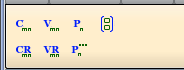
\includegraphics[width=3cm]{./fig/Tut05-01.png}
\end{center}
Los significados son evidentes, así que nos limitamos a invitarte  a que uses Wiris para calcular
el resultado de estos ejercicios:
     \begin{ejercicio}
\label{tut03:ejercicio14}
\quad
\begin{enumerate}
\item Permutaciones de 6 elementos.
\item Variaciones de 100 elementos, tomados de 30 en 30.
\item Combinaciones de 22 elementos, tomados de 7 en 7.
\item Permutaciones con repetición de 10 elementos, divididos en grupos de elementos idénticos de $( 2,2,3,3)$ (de modo que hay $2$ del primer tipo, $2$ del segundo, $3$ del tercero y $3$ del cuarto tipo).
\item Variaciones con repetición de 8 elementos, tomados de 13 en 13.
\item Combinaciones con repetición de 4 elementos tomados de 6 en 6.
\end{enumerate}
Soluciones en la pág. \pageref{tut03:ejercicio14:sol}.
\qed
\end{ejercicio}
Aparte de calcular estos números, puedes usar Wiris para enumerar (es decir, hacer la lista, explícitamente) las variaciones o combinaciones. La forma de hacer esto es darle a Wiris como primer argumento una lista de los valores entre los que tiene que hacer la selección. Por ejemplo, para obtener la lista de variaciones de las 5 letras
\[\{a, b, c, d\}\]
tomadas de 2 en 2 (hay 12 posibles), hacemos esto (se muestra el resultado de ejecutar el comando)
\begin{center}
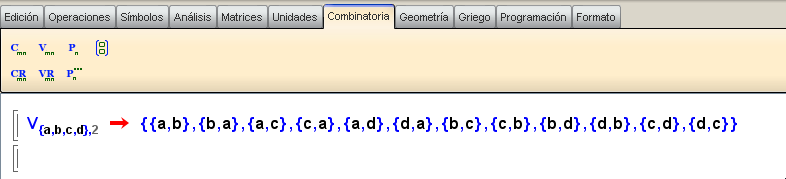
\includegraphics[width=12cm]{./fig/Tut05-07.png}
\end{center}
Puedes aprender más sobre las capacidades combinatorias de Wiris en el manual:
     \begin{center}
\link{http://www.wiris.net/educa.madrid.org/wiris/manual/es/html/tour/combinatoria.html}{http://www.wiris.net/educa.madrid.org/wiris/manual/es/html/tour/combinatoria.html}
\end{center}

\subsection{Wolfram Alpha}
\label{tut03:subsec:CombinatoriaWolframAlpha}

Para usar Wolfram Alpha, debemos expresar (en inglés, claro) lo que deseamos calcular en esa mezcla de lenguaje natural y símbolos matemáticos, característica de este sistema. Por ejemplo, si escribes en el campo de entrada:
     \begin{center}
{\tt number of permutations of 23 elements}
\end{center}
obtendrás como respuesta
\begin{center}
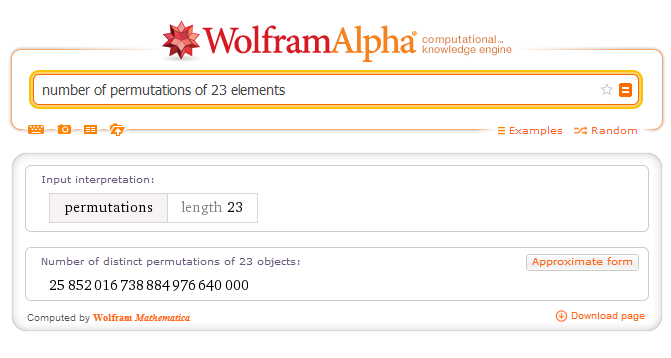
\includegraphics[width=12cm]{./fig/Tut05-08.png}
\end{center}
Si quieres copiar el resultado para poder pegarlo en otro programa, sitúa el ratón sobre ese resultado, y verás aparecer una barra de herramientas, como en la siguiente figura. Haz clic en la letra {\tt A} para obtener una versión copiable como texto del resultado.
\begin{center}
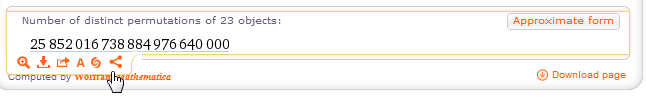
\includegraphics[width=12cm]{./fig/Tut05-09.png}
\end{center}
Para ver más ejemplos de como usar Wolfram Alpha en Combinatoria, teclea {\tt Combinatorics} en la línea de entrada. Ten en cuenta, en cualquier caso, que muchos de los ejemplos que verás no son relevantes para nuestro curso. Así que asegúrate de, al menos, hacer el siguiente
\begin{ejercicio}
\label{tut03:ejercicio15}
\quad
Teclea en el campo de entrada de Wolfram Alpha los siguientes comandos y, para practicar, copia el resultado como texto en un editor de texto, como el Bloc de Notas.
\begin{enumerate}
\item {\tt permutations of 6 elements}
\item {\tt permutations(100,30)}
\item {\tt combinations(22,7)}
\item {\tt number of permutations of {a,a,b,b,c,c,c,d,d,d}}
\item Aunque no hay una sintaxis directa (al menos, yo no la conozco), usa Wolpram Alpha para calcular el número de variaciones con repetición de 8 elementos, tomados de 13 en 13, y el de combinaciones con repetición de 4 elementos tomados de 6 en 6.
\end{enumerate}
Soluciones en la pág. \pageref{tut03:ejercicio15:sol}.
\qed
\end{ejercicio}


\section{Ejercicios adicionales y soluciones}
\label{tut03:sec:SolucionesEjerciciosAdicionales}

\subsection*{Ejercicios adicionales}
\label{tut03:subsec:EjerciciosAdicionales}

\begin{enumerate}
\addtocounter{enumi}{16}

%17 
\item \label{tut03:ejercicio17} Se lanzan dos dados. Hallar la probabilidad de estos sucesos:
\begin{enumerate}
     \item la suma de los resultados es ocho y (simultáneamente) su diferencia es cuatro.
     \item la suma de los resultados es cinco y (simultáneamente) su producto es cuatro.
     \item la suma de los resultados sea mayor que 12.
     \item la suma de los resultados sea divisible entre 3.
\end{enumerate}
Solución en la página \pageref{tut03:ejercicio17:sol}. 


%18
\item  \label{tut03:ejercicio18} Hallar la probabilidad de que al lanzar una moneda dos veces se obtenga al menos una vez una cruz.
Solución en la página \pageref{tut03:ejercicio18:sol}. 


%19 
\item \label{tut03:ejercicio19} En una caja hay seis fichas iguales numeradas del uno al 6. Se extraen una por una (sin reemplazarlas) todas las fichas de la caja. ¿Cuál es la probabilidad de que salgan en el orden natural? (Es decir, primero la ficha número uno, luego la dos, etc.)     
Solución en la página \pageref{tut03:ejercicio19:sol}. 


     
     %20
\item  \label{tut03:ejercicio20} En un paquete hay 20 tarjetas numeradas del 1 al 20. Se escogen al azar dos tarjetas. ¿Cuál es la probabilidad de que las dos que se han elegido sean la número 1 y la número 20? ¿Hay alguna diferencia entre sacar las dos tarjetas a la vez, o sacarlas consecutivamente sin reemplazamiento? ¿Y si es con reemplazamiento (sacamos una, la devolvemos al paquete y sacamos otra al azar)?      
Solución en la página \pageref{tut03:ejercicio20:sol}.


%21
\item  \label{tut03:ejercicio21} Una clase consta de 10 hombres y 20 mujeres. La mitad de los hombres y la mitad de las mujeres tienen los ojos castaños. Hallar la probabilidad de que una persona elegida al azar sea un hombre o tenga los ojos castaños. 
Solución en la página \pageref{tut03:ejercicio21:sol}. 

%22
\item \label{tut03:ejercicio22} Las siguientes afirmaciones son necesariamente falsas. Explica por qué.
\begin{enumerate}
     \item En un hospital, la probabilidad de que un paciente permanezca ingresado durante m\'as de dos d\'ias  es de 0.5. La probabilidad de que un paciente permanezca hospitalizado durante m\'as de un d\'ia es de 0.3.
     \item La probabilidad de que llueva el s\'abado es del 50\% y de que llueva el domingo es del 50\%. Por tanto, durante el fin de semana es seguro que llover\'a.
\end{enumerate}
Solución en la página \pageref{tut03:ejercicio22:sol}. 



%23
\item \label{tut03:ejercicio23} Se escogen al azar tres lámparas de entre 15, y sabemos que de esas 15, cinco son defectuosas. ¿Cuál es la probabilidad de que al menos una de las tres elegidas sea defectuosa? 
Solución en la página \pageref{tut03:ejercicio23:sol}.   

%24
\item \label{tut03:ejercicio24} Hallar la probabilidad de que al tirar tres dados aparezca el seis en uno de los dados (no importa cual), pero sólo en uno de ellos.     
Solución en la página \pageref{tut03:ejercicio24:sol}. 


%25
\item \label{tut03:ejercicio25} En una baraja de cartas espa\~nola (40 cartas repartidas entre 4 palos) se desechan un n\'umero de cartas indeterminado. De las cartas que quedan se tiene una serie de probabilidades a la hora de sacar una carta:
$$P(\{\hbox{sacar rey}\})=0.15,\quad P(\{\hbox{sacar bastos}\})=0.3,$$
y adem\'as
$$P(\{\hbox{sacar carta que no sea rey ni bastos}\})=0.6.$$
\begin{enumerate}
     \item ¿Est\'a entre las cartas no desechadas el rey de bastos? En caso afirmativo, calcula la probabilidad de sacar esta carta.
     \item ¿Cu\'antas cartas hay?
\end{enumerate}
Solución en la página \pageref{tut03:ejercicio25:sol}. 


%26
\item  \label{tut03:ejercicio26}  En cierta facultad, se sabe que (1) un 25\% de los estudiantes suspendió Matemáticas, (2) un 15\% suspendió Química y (c) un 10\% suspendió ambas. Se selecciona un estudiante al azar:
\begin{enumerate}
\item si suspendió Química, ¿cuál es la probabilidad de que también suspendiera Matemáticas?
\item si suspendió Matemáticas, ¿cuál es la probabilidad de que también suspendiera Química?
\item ¿Cuál es la probabilidad de que suspendiera al menos una de las dos?
\end{enumerate}
Solución en la página \pageref{tut03:ejercicio26:sol}. 


%28
\item  \label{tut03:ejercicio28} Un hospital tiene dos quirófanos en funcionamiento. En el primero se han producido incidentes en el 20\% de sus operaciones y el segundo sólo en el 4\%. El número de operaciones es el mismo en ambos quirófanos. La inspección hospitalaria analiza el expediente de una operación, elegido  al azar y observa que en esa operación se produjo un incidente. ¿Cuál es la probabilidad de que la operación se realizara en el primer quirófano?
Solución en la página \pageref{tut03:ejercicio28:sol}. 

%    \item En cierta población el porcentaje de personas que padecen una determinada enfermedad es del $2\%$. Para identificar a los enfermos se dispone de una prueba diagnóstica. Esa prueba no es perfecta: resulta positiva en el $95\%$ de las personas que padecen la enfermedad, pero también resulta positiva en el $3\%$ de las personas sanas (falsos positivos).  Calcular la probabilidad de que una persona con prueba positiva padezca realmente la enfermedad.

%29
\item  \label{tut03:ejercicio29} Un equipo de investigación está preparando un nuevo test para el diagnóstico de la enfermedad de Alzheimer. El test se ha probado en una muestra aleatoria con 450 pacientes diagnosticados con Alzheimer y una muestra aleatoria independiente de 500 pacientes que no presentan síntomas de la enfermedad. La siguiente tabla resume los resultados del ensayo:
\begin{center}
\begin{tabular}{llccc}
&&\multicolumn{3}{c}{\underline{\bf Padecen Alzheimer}}\\

&          & Sí  & No  & Total\\
\hline
\underline{\bf Resultado del  Test} & Positivo & 436 & 5   & 441  \\
& Negativo & 14  & 495 & 509  \\
\hline
& Total    & 450 & 500 & 950  \\
\hline
\end{tabular}
\end{center}
Con estos datos, responder a las siguientes preguntas:
\begin{enumerate}
     \item ¿Cuál es la probabilidad de que un sujeto sano haya dado positivo en el test?
     \item ¿Cuál es la probabilidad de que un sujeto enfermo haya dado negativo en el test?
     \item Sabiendo que un sujeto ha dado positivo en el test, ¿cuál es la probabilidad de que esté enfermo?
     \item  Sabiendo que un sujeto ha dado negativo en el test, ¿cuál es la probabilidad de que esté sano?
\end{enumerate}
Solución en la página \pageref{tut03:ejercicio29:sol}. 

%  30
\item  \label{tut03:ejercicio30} Una empresa produce anillas para identificaci\'on de tortugas marinas en tres fábricas. El volumen de producci\'on diario es de 500, 1000 y 2000 unidades respectivamente. Se sabe  que la fracci\'on de producci\'on defectuosa de las tres fábricas es de 0.005, 0.008, 0.010 respectivamente. Si se selecciona una anilla de forma aleatoria del total de producci\'on de un d\'ia y se descubre que es defectuosa, ?`de qu\'e fábrica es más probable que provenga esa anilla?    
Solución en la página \pageref{tut03:ejercicio30:sol}. 


% 31
\item Usa R para simular el experimento que se describe en el Ejemplo \ref{curso-Cap03:probabilidadCondicionadaLanzamientoDosDados} del libro (pág. \pageref{curso-Cap03:probabilidadCondicionadaLanzamientoDosDados}). Por si te sirve de guía visual, en la hoja de cálculo (del programa Calc):
\begin{center} \otrofichero{Cap03-Lanzamientos2Dados-ProbabilidadCondicionada.ods}{Cap03-Lanzamientos2Dados-ProbabilidadCondicionada.ods}
\end{center}
se ha realizado una simulación para comprobar estos resultados.\\
Una extensión natural de este ejemplo es tratar de calcular $P(S|D)$. ¿Puedes modificar la hoja de cálculo para simular este otro caso?

%32
\item  Usa R para simular el experimento que se describe en el Ejemplo \ref{curso-cap03:ejem:ProbailidadTotalEjemploUrnas} del libro (pág. \pageref{curso-cap03:ejem:ProbailidadTotalEjemploUrnas}), y que ilustramos con el fichero  Calc
\begin{center}
\otrofichero{Cap03-ProbabilidadesTotales-Urnas.ods}{Cap03-ProbabilidadesTotales-Urnas.ods}
\end{center}
%33
\item Usa R para simular los experimentos de los Ejemplos \ref{curso-cap03:ejem:BombillasDefectuosas} y \ref{curso-cap03:ejem:probabilidadLanzamientoMonedas} del libro (pág. \pageref{curso-cap03:ejem:BombillasDefectuosas})


% 34
\item  \label{tut03:ejercicio34} Elegimos al azar cinco números del $1$ al $10$, con reemplazamiento. Puedes pensarlo así: en una caja hay $10$ bolas numeradas del $1$ al $10$. Sacamos una bola, anotamos el número, devolvemos la bola a la caja, y la agitamos bien. ¿Cuál es la probabilidad de que no haya repeticiones y, por tanto, obtengamos cinco números distintos?
Solución en la página \pageref{tut03:ejercicio34:sol}. 


%35
\item  \label{tut03:ejercicio35} De entre los números naturales $1,2,\ldots,20$ se seleccionan cinco al azar sin reemplazamiento. Calcular la probabilidad de que: (a) los cinco sean pares. (b) exactamente dos de ellos sean múltiplos de 3. (c) dos sean impares y tres pares. 
Solución en la página \pageref{tut03:ejercicio35:sol}. 

% 36 
   \item \label{tut03:ejercicio36}  En la lotería primitiva gana quien acierta 6 números de entre 64 sin importar el orden en el que salgan. ¿Cuál es la probabilidad de ganar con una única apuesta? 
Solución en la página \pageref{tut03:ejercicio36:sol}. 

% 37
\item  \label{tut03:ejercicio37} De las 28 fichas del dominó, se extraen dos al azar (sin remplazamiento). ¿Cuál es la probabilidad de que con ellas se pueda formar una cadena, conforme a las reglas del juego (debe haber un número que aparezca en ambas fichas)?
Solución en la página \pageref{tut03:ejercicio37:sol}. 


%38
\item  \label{tut03:ejercicio38} Calcular la probabilidad de que un número de cuatro cifras (una matrícula, o un pin)
\begin{enumerate}
\item tenga cuatro cifras diferentes.
\item tenga alguna cifra repetida.
\item tenga exactamente dos cifras iguales.
\item tenga dos parejas de cifras iguales (pero distintas entre sí).
\item tenga exactamente tres cifras iguales.
\item tenga todas las cifras iguales.
\end{enumerate}
Solución en la página \pageref{tut03:ejercicio38:sol}. 

% 39
\item \label{tut03:ejercicio39} {\bf ``La paradoja del cumpleaños''.} Si en una sala hay $367$ personas, entonces, con total seguridad, habrá dos personas con la misma fecha de cumpleaños (hemos usado $367$ para cubrir incluso el caso de los años bisiestos, por si alguien de la sala nació el $29$ de Febrero). Así que, si llamamos
$$A_n= \{\mbox{al menos dos de las $n$ personas cumplen años el mismo día}\}$$
entonces $P(A_{367})=1$. ¿Cuántas personas tiene que haber en la sala para que la probabilidad $P(A_{n})$ sea mayor que $1/2$? Muchas menos de las que imaginas. Empieza por calcular ¿Cuánto vale $P(A_{5})$ usando el ejercicio anterior.\\
Este resultado se conoce como ``la paradoja del cumpleaños'', aunque no tiene nada de paradójico. Lo único que realmente demuestra este resultado es que, como hemos señalado en el curso, la intuición en materia de probabilidades es, en general, para la mayoría de nosotros, muy pobre.%\\
Solución en la página \pageref{tut03:ejercicio39:sol}. 

\end{enumerate}

\subsection*{Soluciones de algunos ejercicios}

\paragraph{\bf $\bullet$ Ejercicio \ref{tut03:ejercicio01}, pág. \pageref{tut03:ejercicio01}}
\label{tut03:ejercicio01:sol}\quad\\

\begin{knitrout}
\definecolor{shadecolor}{rgb}{0.969, 0.969, 0.969}\color{fgcolor}\begin{kframe}
\begin{alltt}
\hlkwd{set.seed}\hlstd{(}\hlnum{2014}\hlstd{)}
\hlstd{(caja}\hlkwb{=}\hlkwd{rep}\hlstd{(} \hlnum{1}\hlopt{:}\hlnum{5}\hlstd{,} \hlkwd{c}\hlstd{(}\hlnum{35}\hlstd{,} \hlnum{15}\hlstd{,} \hlnum{10}\hlstd{,} \hlnum{10}\hlstd{,} \hlnum{30}\hlstd{) ))}
\end{alltt}
\begin{verbatim}
##   [1] 1 1 1 1 1 1 1 1 1 1 1 1 1 1 1 1 1 1 1 1 1 1 1 1 1 1 1 1 1 1 1 1 1 1 1
##  [36] 2 2 2 2 2 2 2 2 2 2 2 2 2 2 2 3 3 3 3 3 3 3 3 3 3 4 4 4 4 4 4 4 4 4 4
##  [71] 5 5 5 5 5 5 5 5 5 5 5 5 5 5 5 5 5 5 5 5 5 5 5 5 5 5 5 5 5 5
\end{verbatim}
\begin{alltt}
\hlstd{(sorteo1} \hlkwb{=} \hlkwd{sample}\hlstd{(caja,} \hlnum{20}\hlstd{,} \hlkwc{replace} \hlstd{=} \hlnum{TRUE}\hlstd{))}
\end{alltt}
\begin{verbatim}
##  [1] 1 1 4 1 3 1 5 4 1 1 4 1 4 3 4 2 4 1 5 1
\end{verbatim}
\begin{alltt}
\hlstd{(sorteo2} \hlkwb{=} \hlkwd{sample}\hlstd{(caja,} \hlnum{20}\hlstd{,} \hlkwc{replace} \hlstd{=} \hlnum{FALSE}\hlstd{))}
\end{alltt}
\begin{verbatim}
##  [1] 5 4 3 5 4 5 2 2 1 5 5 1 2 1 5 3 5 4 5 3
\end{verbatim}
\begin{alltt}
\hlstd{(tabFrecAbs1}  \hlkwb{=} \hlkwd{table}\hlstd{(sorteo1))}
\end{alltt}
\begin{verbatim}
## sorteo1
## 1 2 3 4 5 
## 9 1 2 6 2
\end{verbatim}
\begin{alltt}
\hlstd{(tabFrecRel1}  \hlkwb{=} \hlkwd{table}\hlstd{(sorteo1)} \hlopt{/} \hlkwd{length}\hlstd{(sorteo1) )}
\end{alltt}
\begin{verbatim}
## sorteo1
##    1    2    3    4    5 
## 0.45 0.05 0.10 0.30 0.10
\end{verbatim}
\begin{alltt}
\hlstd{(tabFrecAbs2}  \hlkwb{=} \hlkwd{table}\hlstd{(sorteo2))}
\end{alltt}
\begin{verbatim}
## sorteo2
## 1 2 3 4 5 
## 3 3 3 3 8
\end{verbatim}
\begin{alltt}
\hlstd{(tabFrecRel2}  \hlkwb{=} \hlkwd{table}\hlstd{(sorteo2)} \hlopt{/} \hlkwd{length}\hlstd{(sorteo2) )}
\end{alltt}
\begin{verbatim}
## sorteo2
##    1    2    3    4    5 
## 0.15 0.15 0.15 0.15 0.40
\end{verbatim}
\end{kframe}
\end{knitrout}

\paragraph{\bf $\bullet$ Ejercicio \ref{tut03:ejercicio02}, pág. \pageref{tut03:ejercicio02}}
\label{tut03:ejercicio02:sol}\quad\\

Cuando {\tt byrow=FALSE} (que es la opción por defecto), los elementos se colocan por columnas.
\begin{knitrout}
\definecolor{shadecolor}{rgb}{0.969, 0.969, 0.969}\color{fgcolor}\begin{kframe}
\begin{alltt}
\hlstd{(dosPartidas} \hlkwb{=} \hlkwd{matrix}\hlstd{(}\hlkwd{head}\hlstd{(dado4000,} \hlnum{8}\hlstd{),} \hlkwc{ncol} \hlstd{=} \hlnum{4}\hlstd{,} \hlkwc{byrow} \hlstd{=} \hlnum{FALSE}\hlstd{))}
\end{alltt}
\begin{verbatim}
##      [,1] [,2] [,3] [,4]
## [1,]    2    4    4    6
## [2,]    2    2    1    4
\end{verbatim}
\begin{alltt}
\hlstd{(dosPartidas} \hlkwb{=} \hlkwd{matrix}\hlstd{(}\hlkwd{head}\hlstd{(dado4000,} \hlnum{8}\hlstd{),} \hlkwc{ncol} \hlstd{=} \hlnum{4}\hlstd{))}
\end{alltt}
\begin{verbatim}
##      [,1] [,2] [,3] [,4]
## [1,]    2    4    4    6
## [2,]    2    2    1    4
\end{verbatim}
\end{kframe}
\end{knitrout}


\paragraph{\bf $\bullet$ Ejercicio \ref{tut03:ejercicio03}, pág. \pageref{tut03:ejercicio03}}
\label{tut03:ejercicio03:sol}\quad\\

\begin{knitrout}
\definecolor{shadecolor}{rgb}{0.969, 0.969, 0.969}\color{fgcolor}\begin{kframe}
\begin{alltt}
\hlstd{(M} \hlkwb{=} \hlkwd{matrix}\hlstd{(}\hlnum{1}\hlopt{:}\hlnum{36}\hlstd{,} \hlkwc{nrow}\hlstd{=}\hlnum{4}\hlstd{,} \hlkwc{byrow}\hlstd{=}\hlnum{TRUE}\hlstd{) )}
\end{alltt}
\begin{verbatim}
##      [,1] [,2] [,3] [,4] [,5] [,6] [,7] [,8] [,9]
## [1,]    1    2    3    4    5    6    7    8    9
## [2,]   10   11   12   13   14   15   16   17   18
## [3,]   19   20   21   22   23   24   25   26   27
## [4,]   28   29   30   31   32   33   34   35   36
\end{verbatim}
\end{kframe}
\end{knitrout}

\paragraph{\bf $\bullet$ Ejercicio \ref{tut03:ejercicio04}, pág. \pageref{tut03:ejercicio04}}
\label{tut03:ejercicio04:sol}\quad\\

\begin{knitrout}
\definecolor{shadecolor}{rgb}{0.969, 0.969, 0.969}\color{fgcolor}\begin{kframe}
\begin{alltt}
\hlkwd{dim}\hlstd{(M)}\hlkwb{=} \hlkwd{c}\hlstd{(}\hlnum{4}\hlstd{,} \hlnum{9}\hlstd{)}
\hlstd{M}
\end{alltt}
\begin{verbatim}
##      [,1] [,2] [,3] [,4] [,5] [,6] [,7] [,8] [,9]
## [1,]    1    2    3    4    5    6    7    8    9
## [2,]   10   11   12   13   14   15   16   17   18
## [3,]   19   20   21   22   23   24   25   26   27
## [4,]   28   29   30   31   32   33   34   35   36
\end{verbatim}
\end{kframe}
\end{knitrout}

\paragraph{\bf $\bullet$ Ejercicio \ref{tut03:ejercicio05}, pág. \pageref{tut03:ejercicio05}}
\label{tut03:ejercicio05:sol}\quad\\

Los vectores {\em puros} de R no tienen dimensión cuando son creados. La adquieren al convertirlos en matrices.
\begin{knitrout}
\definecolor{shadecolor}{rgb}{0.969, 0.969, 0.969}\color{fgcolor}\begin{kframe}
\begin{alltt}
\hlstd{unVector} \hlkwb{=} \hlnum{1}\hlopt{:}\hlnum{10}
\hlkwd{dim}\hlstd{(unVector)}
\end{alltt}
\begin{verbatim}
## NULL
\end{verbatim}
\begin{alltt}
\hlkwd{class}\hlstd{(unVector)}
\end{alltt}
\begin{verbatim}
## [1] "integer"
\end{verbatim}
\begin{alltt}
\hlstd{M} \hlkwb{=} \hlkwd{matrix}\hlstd{(unVector,} \hlkwc{nrow}\hlstd{=}\hlnum{1}\hlstd{)}
\hlkwd{dim}\hlstd{(M)}
\end{alltt}
\begin{verbatim}
## [1]  1 10
\end{verbatim}
\begin{alltt}
\hlkwd{class}\hlstd{(M)}
\end{alltt}
\begin{verbatim}
## [1] "matrix"
\end{verbatim}
\begin{alltt}
\hlstd{a}\hlkwb{=}\hlstd{letters[}\hlnum{1}\hlopt{:}\hlnum{12}\hlstd{]}
\hlstd{(Ma} \hlkwb{=} \hlkwd{matrix}\hlstd{(a,} \hlkwc{nrow}\hlstd{=}\hlnum{3}\hlstd{))}
\end{alltt}
\begin{verbatim}
##      [,1] [,2] [,3] [,4]
## [1,] "a"  "d"  "g"  "j" 
## [2,] "b"  "e"  "h"  "k" 
## [3,] "c"  "f"  "i"  "l"
\end{verbatim}
\end{kframe}
\end{knitrout}


\paragraph{\bf $\bullet$ Ejercicio \ref{tut03:ejercicio06}, pág. \pageref{tut03:ejercicio06}}
\label{tut03:ejercicio06:sol}\quad\\

\begin{knitrout}
\definecolor{shadecolor}{rgb}{0.969, 0.969, 0.969}\color{fgcolor}\begin{kframe}
\begin{alltt}
\hlstd{(letras} \hlkwb{=} \hlkwd{matrix}\hlstd{(letters[}\hlnum{1}\hlopt{:}\hlnum{12}\hlstd{],} \hlkwc{nrow}\hlstd{=}\hlnum{4}\hlstd{,} \hlkwc{byrow}\hlstd{=}\hlnum{TRUE}\hlstd{))}
\end{alltt}
\begin{verbatim}
##      [,1] [,2] [,3]
## [1,] "a"  "b"  "c" 
## [2,] "d"  "e"  "f" 
## [3,] "g"  "h"  "i" 
## [4,] "j"  "k"  "l"
\end{verbatim}
\begin{alltt}
\hlkwd{dim}\hlstd{(letras)}
\end{alltt}
\begin{verbatim}
## [1] 4 3
\end{verbatim}
\begin{alltt}
\hlkwd{dim}\hlstd{(letras)}\hlkwb{=}\hlkwd{c}\hlstd{(}\hlnum{3}\hlstd{,}\hlnum{4}\hlstd{)}
\hlstd{letras}
\end{alltt}
\begin{verbatim}
##      [,1] [,2] [,3] [,4]
## [1,] "a"  "j"  "h"  "f" 
## [2,] "d"  "b"  "k"  "i" 
## [3,] "g"  "e"  "c"  "l"
\end{verbatim}
\end{kframe}
\end{knitrout}

\paragraph{\bf $\bullet$ Ejercicio \ref{tut03:ejercicio07}, pág. \pageref{tut03:ejercicio07}}
\label{tut03:ejercicio07:sol}\quad\\


La comprobación es:
\begin{knitrout}
\definecolor{shadecolor}{rgb}{0.969, 0.969, 0.969}\color{fgcolor}\begin{kframe}
\begin{alltt}
\hlkwd{t}\hlstd{(W)}
\end{alltt}
\begin{verbatim}
##      [,1] [,2] [,3]
## [1,]    1    6   11
## [2,]    2    7   12
## [3,]    3    8   13
## [4,]    4    9   14
## [5,]    5   10   15
\end{verbatim}
\begin{alltt}
\hlkwd{dim}\hlstd{(W)} \hlkwb{=} \hlkwd{c}\hlstd{(}\hlnum{5}\hlstd{,}\hlnum{3}\hlstd{)}
\hlstd{W}
\end{alltt}
\begin{verbatim}
##      [,1] [,2] [,3]
## [1,]    1   12    9
## [2,]    6    3   14
## [3,]   11    8    5
## [4,]    2   13   10
## [5,]    7    4   15
\end{verbatim}
\end{kframe}
\end{knitrout}



\paragraph{\bf $\bullet$ Ejercicio \ref{tut03:ejercicio07a}, pág. \pageref{tut03:ejercicio07a}}
\label{tut03:ejercicio07a:sol}\quad\\


\begin{knitrout}
\definecolor{shadecolor}{rgb}{0.969, 0.969, 0.969}\color{fgcolor}\begin{kframe}
\begin{alltt}
\hlkwd{apply}\hlstd{(M,} \hlnum{1}\hlstd{, sd)}
\end{alltt}
\begin{verbatim}
## [1] 2.74 2.74 2.74 2.74
\end{verbatim}
\begin{alltt}
\hlkwd{apply}\hlstd{(M,} \hlnum{2}\hlstd{, median)}
\end{alltt}
\begin{verbatim}
## [1] 14.5 15.5 16.5 17.5 18.5 19.5 20.5 21.5 22.5
\end{verbatim}
\begin{alltt}
\hlkwd{apply}\hlstd{(M,} \hlnum{2}\hlstd{, summary)}
\end{alltt}
\begin{verbatim}
##          [,1]  [,2]  [,3] [,4] [,5] [,6] [,7] [,8] [,9]
## Min.     1.00  2.00  3.00  4.0  5.0  6.0  7.0  8.0  9.0
## 1st Qu.  7.75  8.75  9.75 10.8 11.8 12.8 13.8 14.8 15.8
## Median  14.50 15.50 16.50 17.5 18.5 19.5 20.5 21.5 22.5
## Mean    14.50 15.50 16.50 17.5 18.5 19.5 20.5 21.5 22.5
## 3rd Qu. 21.20 22.20 23.20 24.2 25.2 26.2 27.2 28.2 29.2
## Max.    28.00 29.00 30.00 31.0 32.0 33.0 34.0 35.0 36.0
\end{verbatim}
\begin{alltt}
\hlkwd{class}\hlstd{(}\hlkwd{apply}\hlstd{(M,} \hlnum{2}\hlstd{, summary))}
\end{alltt}
\begin{verbatim}
## [1] "matrix"
\end{verbatim}
\end{kframe}
\end{knitrout}


\paragraph{\bf $\bullet$ Ejercicio \ref{tut03:ejercicio08}, pág. \pageref{tut03:ejercicio08}}
\label{tut03:ejercicio08:sol}\quad\\




\begin{enumerate}
\item La matriz que buscamos es:
\begin{knitrout}
\definecolor{shadecolor}{rgb}{0.969, 0.969, 0.969}\color{fgcolor}\begin{kframe}
\begin{alltt}
\hlstd{B} \hlopt{==} \hlnum{2}
\end{alltt}
\begin{verbatim}
##       [,1]  [,2]  [,3]  [,4]
## [1,]  TRUE FALSE FALSE FALSE
## [2,]  TRUE FALSE FALSE FALSE
## [3,] FALSE FALSE FALSE FALSE
\end{verbatim}
\end{kframe}
\end{knitrout}

\item Se produce un error, porque al tratarse de matrices de dimensiones distintas, R no sabe como emparejar los elementos de {\tt A} con los de {\tt B}.
\begin{knitrout}
\definecolor{shadecolor}{rgb}{0.969, 0.969, 0.969}\color{fgcolor}\begin{kframe}
\begin{alltt}
\hlkwd{dim}\hlstd{(A)} \hlkwb{=} \hlkwd{c}\hlstd{(}\hlnum{2}\hlstd{,} \hlnum{6}\hlstd{)}
\hlstd{A} \hlopt{*} \hlstd{B}
\end{alltt}


{\ttfamily\noindent\bfseries\color{errorcolor}{\#\# Error in A * B: arreglos de dimens'on no compatibles}}\end{kframe}
\end{knitrout}


\end{enumerate}



\paragraph{\bf $\bullet$ Ejercicio \ref{tut03:ejercicio09}, pág. \pageref{tut03:ejercicio09}}
\label{tut03:ejercicio09:sol}\quad\\


\begin{knitrout}
\definecolor{shadecolor}{rgb}{0.969, 0.969, 0.969}\color{fgcolor}\begin{kframe}
\begin{alltt}
\hlstd{(B} \hlkwb{=} \hlkwd{cbind}\hlstd{(A, A[,} \hlnum{1}\hlstd{]}\hlopt{^}\hlnum{2}\hlstd{))}
\end{alltt}
\begin{verbatim}
##      [,1] [,2] [,3] [,4] [,5] [,6] [,7]
## [1,]   -4    3    1    9   -8    3   16
## [2,]   -7   -4   -9    2   -7   -9   49
\end{verbatim}
\end{kframe}
\end{knitrout}


\paragraph{\bf $\bullet$ Ejercicio \ref{tut03:ejercicio10}, pág. \pageref{tut03:ejercicio10}}
\label{tut03:ejercicio10:sol}\quad\\

\begin{knitrout}
\definecolor{shadecolor}{rgb}{0.969, 0.969, 0.969}\color{fgcolor}\begin{kframe}
\begin{alltt}
\hlkwd{which}\hlstd{(}\hlkwd{rowSums}\hlstd{(esSeis)} \hlopt{==} \hlkwd{max}\hlstd{(}\hlkwd{rowSums}\hlstd{(esSeis)))}
\end{alltt}
\begin{verbatim}
## [1] 602
\end{verbatim}
\end{kframe}
\end{knitrout}

\paragraph{\bf $\bullet$ Ejercicio \ref{tut03:ejercicio11}, pág. \pageref{tut03:ejercicio11}}
\label{tut03:ejercicio11:sol}\quad\\

Puedes ejecutar varias veces este código (que puedes abrir en el fichero adjunto \otrofichero{Tut03-DeMere2.R}{Tut03-DeMere2.R}) para experimentar.

\begin{knitrout}
\definecolor{shadecolor}{rgb}{0.969, 0.969, 0.969}\color{fgcolor}\begin{kframe}


{\ttfamily\noindent\color{warningcolor}{\#\# Warning in file(con, "{}r"{}): no fue posible abrir el archivo './datos/Tut03-DeMere2.R': No such file or directory}}

{\ttfamily\noindent\bfseries\color{errorcolor}{\#\# Error in file(con, "{}r"{}): no se puede abrir la conexi'on}}\end{kframe}
\end{knitrout}



\paragraph{\bf $\bullet$ Ejercicio \ref{tut03:ejercicio12}, pág. \pageref{tut03:ejercicio12}}
\label{tut03:ejercicio12:sol}\quad\\

El código (que puedes abrir en el fichero adjunto \otrofichero{Tut03-DeMere1a.R}{Tut03-DeMere1a.R}) es una adaptación sencilla del que corresponde al primer juego del Caballero de Méré. Puedes ejecutarlo varias veces para comprobar que el resultado se parece más a $\frac{11}{36}\approx0.306$ que a $\frac{12}{36}\approx0.333$.
\begin{knitrout}
\definecolor{shadecolor}{rgb}{0.969, 0.969, 0.969}\color{fgcolor}\begin{kframe}


{\ttfamily\noindent\color{warningcolor}{\#\# Warning in file(con, "{}r"{}): no fue posible abrir el archivo './datos/Tut03-DeMere1a.R': No such file or directory}}

{\ttfamily\noindent\bfseries\color{errorcolor}{\#\# Error in file(con, "{}r"{}): no se puede abrir la conexi'on}}\end{kframe}
\end{knitrout}





\paragraph{\bf $\bullet$ Ejercicio \ref{tut03:ejercicio13}, pág. \pageref{tut03:ejercicio13}}
\label{tut03:ejercicio13:sol}\quad\\

Puedes averiguarlo preguntando a R de esta forma:
\begin{knitrout}
\definecolor{shadecolor}{rgb}{0.969, 0.969, 0.969}\color{fgcolor}\begin{kframe}
\begin{alltt}
\hlkwd{class}\hlstd{(}\hlkwd{permutations}\hlstd{(}\hlnum{4}\hlstd{,}\hlnum{3}\hlstd{) )}
\end{alltt}
\begin{verbatim}
## [1] "matrix"
\end{verbatim}
\begin{alltt}
\hlkwd{class}\hlstd{(}\hlkwd{combinations}\hlstd{(}\hlnum{4}\hlstd{,}\hlnum{3}\hlstd{) )}
\end{alltt}
\begin{verbatim}
## [1] "matrix"
\end{verbatim}
\end{kframe}
\end{knitrout}
Como puedes ver, lo que hemos obtenido es un objeto de tipo {\tt matrix}.


\paragraph{\bf $\bullet$ Ejercicio \ref{tut03:ejercicio14}, pág. \pageref{tut03:ejercicio14}}
\label{tut03:ejercicio14:sol}\quad\\

\begin{enumerate}
\item $720$.
\item $7791097137057804874587232499277321440358327700684800000000$.
Este número podría representar el número de subgrupos distintos de 30 alumnos, que podemos formar a partir de una clase de 100 alumnos. Su orden de magnitud es de $10^{57}$. Para que te hagas una idea, el número estimado de estrellas en el universo es del orden de $10^{24}$.
\item $170544$.
\item $25200$.
\item $549755813888$.
\item $84$.
\end{enumerate}

\paragraph{\bf $\bullet$ Ejercicio \ref{tut03:ejercicio15}, pág. \pageref{tut03:ejercicio15}}
\label{tut03:ejercicio15:sol}\quad\\

Todas las preguntas aparecen en el Ejercicio \ref{tut03:ejercicio14}; consulta las respuesta a ese ejercicio.


%17 
\paragraph{\bf $\bullet$ Ejercicio \ref{tut03:ejercicio17}, pág. \pageref{tut03:ejercicio17}}
\label{tut03:ejercicio17:sol}\quad\\


Se trata de contar casos favorables y casos posibles. 
\begin{enumerate}
\item Una posibilidad consiste en escribir todo el espacio muestral y contar a mano.
\[\begin{array}{rrrrrr}
  (1,1)&(1,2)&(1,3)&(1,4)&(1,5)&{(1,6)}\\
  (2,1)&(2,2)&(2,3)&(2,4)&(2,5)&{(2,6)}\\
  (3,1)&(3,2)&(3,3)&(3,4)&(3,5)&{(3,6)}\\
  (4,1)&(4,2)&(4,3)&(4,4)&(4,5)&{(4,6)}\\
  (5,1)&(5,2)&(5,3)&(5,4)&(5,5)&{(5,6)}\\
  (6,1)&(6,2)&(6,3)&(6,4)&(6,5)&{(6,6)}
  \end{array} \]
 Otra posibilidad consiste en llamar $x_i$ al resultado del lanzamiento $i$. Lo que nos dice el enunciado es que 
\[\left\{\begin{array}{ll}
         x_1+x_2=8\\
         |x_1-x_2|=4
         \end{array}        
         \right.\]
donde las barras de valor absoluto estan para tener en cuenta la posibilidad de que, al restar el resultado de las dos caras del dado, la segunda sea mayor que la primera y el resultdo sea $-4$. Al eliminar el símbolo de valor absoluto, ese sistema de  ecuaciones es equivalente a
\[\left\{\begin{array}{ll}
         x_1+x_2=8\\
         x_1-x_2=4
         \end{array}\right.,\qquad \qquad 
         \left\{
              \begin{array}{ll}
               x_1+x_2=8\\
               x_1-x_2=-4
               \end{array}\right.\]
Al resolver cada uno de los sistemas tenemos $x_1=6, x_2=2$ y  $x_1=2, x_2=6$. Es decir, dos casos favorables frente a 36 posibles. 
\item Análogo al anterior
\item No es posible
\item Debe ser $x_1+x_2=3n$, donde $n$ sólo puede valer $n=1,2,3,4$. La probabilidad es $\frac{12}{36} $
 \end{enumerate}

%18
\paragraph{\bf $\bullet$ Ejercicio \ref{tut03:ejercicio18}, pág. \pageref{tut03:ejercicio18}}
\label{tut03:ejercicio18:sol}\quad\\
Si escribes el espacio muestral, ${(C,C), (C,X), (X,C), (XX)}$ verás que 
hay 4 casos posibles y 3 favorables.

%19 
\paragraph{\bf $\bullet$ 
                Ejercicio \ref{tut03:ejercicio19}, pág. 
           \pageref{tut03:ejercicio19}}
\label{tut03:ejercicio19:sol}\quad\\
Hay 1 caso favorable y $6!$ casos posibles, por lo que la probabilidad es $\frac{1}{6!}$ donde puedes calcular $6!$ con la orden
\begin{knitrout}
\definecolor{shadecolor}{rgb}{0.969, 0.969, 0.969}\color{fgcolor}\begin{kframe}
\begin{alltt}
     \hlkwd{factorial}\hlstd{(}\hlnum{6}\hlstd{)}
\end{alltt}
\begin{verbatim}
## [1] 720
\end{verbatim}
\end{kframe}
\end{knitrout}
     
%20
\paragraph{\bf $\bullet$ Ejercicio \ref{tut03:ejercicio20}, pág. \pageref{tut03:ejercicio20}}
\label{tut03:ejercicio20:sol}\quad\\ 
\begin{itemize}
\item Empezamos suponiendo que sacamos dos fichas a la vez. Usaremos la regla de Laplace para calcular la probabilidad. Hay un caso favorable, que es sacar ${1,20}$. Observa que el orden NO es importante, nos da lo mismo sacar ${1,20}$ que ${20, 1}$. El n\'umero de casos posibles esel n\'umero de subconjuntos de dos tarjetas que podemos hacer a partir de 20 tarjetas, sin que importe el orden. Es decir, combinaciones de 20 elementos tomados de 2 en 2. Podemos usar R para hacer el cálculo con la función `choose()`. Si no recuerdas su significado, usa el tabulador
\begin{knitrout}
\definecolor{shadecolor}{rgb}{0.969, 0.969, 0.969}\color{fgcolor}\begin{kframe}
\begin{alltt}
\hlnum{1}\hlopt{/}\hlkwd{choose}\hlstd{(}\hlnum{20}\hlstd{,}\hlnum{2}\hlstd{)}
\end{alltt}
\begin{verbatim}
## [1] 0.00526
\end{verbatim}
\end{kframe}
\end{knitrout}
\item Supongamos ahora que sacamos las dos fichas una tras otra SIN reemplazamiento. En este caso debemos tener en cuenta el orden, ya que el experimento tendría resultado positivo tanto si primero sale un 1 y despues el 20 como si sucediera al revés.  
$$P(A=\text{sacar primero un 1 y después un 20}) = P(\text{sacar un 1})· 
P(\text{sacar un 20}|\text{ha salido un 1})$$
$$=\frac{1}{20}\frac{1}{19} $$
De la misma manera, 
$$P(B=\text{sacar primero un 20 y después un 1}) =\frac{1}{20}\frac{1}{19} $$
Y la probabilidad total es 
\begin{knitrout}
\definecolor{shadecolor}{rgb}{0.969, 0.969, 0.969}\color{fgcolor}\begin{kframe}
\begin{alltt}
\hlstd{(}\hlnum{1}\hlopt{/}\hlnum{20}\hlstd{)}\hlopt{*}\hlstd{(}\hlnum{1}\hlopt{/}\hlnum{19}\hlstd{)}\hlopt{+}\hlstd{(}\hlnum{1}\hlopt{/}\hlnum{20}\hlstd{)}\hlopt{*}\hlstd{(}\hlnum{1}\hlopt{/}\hlnum{19}\hlstd{)}
\end{alltt}
\begin{verbatim}
## [1] 0.00526
\end{verbatim}
\end{kframe}
\end{knitrout}
\item Vamos a usar un razonamiento diferente para este último caso (pero que se puede aplicar a los anteriores, y recíprocamente, el argumento con el que resolvimos los anteriores apartados se puede aplicar a este) 
$$P(\text{sacar un 1 y un 20}) = P(\text{sacar un 1 o un 20})· 
P(\text{sacar la ficha que falta | ya salió un 1 o un 20})$$
$$=\frac{\textbf{2}}{20}\frac{1}{\textbf{20}} $$
porque se ha devuelto la primera ficha, de modo que las probabilidades con y sin reemplazamiento son diferentes.
\end{itemize}

%21
\paragraph{\bf $\bullet$ Ejercicio \ref{tut03:ejercicio21}, pág. \pageref{tut03:ejercicio21}}
\label{tut03:ejercicio21:sol}\quad\\
Hay varios enfoques posibles. Uno de ellos, el m\'as sistem\'atico, 
consiste en definir los eventos 
\[H=\text{"ser hombre"}\qquad\qquad
  C=\text{"tenerlos ojos marrones"}\]
Con esa notaci\'on, la probabilidad pedida es $P(H\up C)$. 
Un recuento y la regla de Laplace permite determinar que 
\[P(H)=10/30\qquad P(C)=15/30\qquad P(H\cap C)=5/30\]
de donde, usando las reglas de c\'alculo de probabilidades, 
se tiene 
\[P(H\cup C)=P(H)+P(C)-P(H\cap C)=10/30+P(C)=15/30- P(H\cap C)=2/3\]

Una aproximaci\'on alternativa consiste en contar los casos favorables, que son 20 (10 hombre y las 10 mujeres que tienen los ojos castaños) y dividir entre los casos posibles, que son 30, para obtener $$P(\text{ser hombre o tenerlos ojos castaños})=\frac{2}{3}$$


%22
\paragraph{\bf $\bullet$ Ejercicio \ref{tut03:ejercicio22}, pág. \pageref{tut03:ejercicio22}}
\label{tut03:ejercicio22:sol}\quad\\

\begin{enumerate}
\item El evento ''permanecer ingresado durante m\'as de dos d\'ias'' está contenido (estrictamente) en el evento ''permanecer  hospitalizado durante m\'as de un d\'ia'', en el sentido de que si alguien está hospitalizado 2 díaso más ha tenidoque estar (forzosamente) hospitalizado un día o más. Por tanto, el primero no puede tener una probabilidad (estríctamente) mayor que el segundo.
\item Los eventos S = ''que llueva el sábado'' y  D = ''que llueva el domingo'' son independientes y ambos tiene probabilidad 1/2. 
Por las reglas de la probabilidad 
$$P(\text{llueva el fin de semana})=P(S\cup D) =P(S)+P( D)-P(S\cap D) =$$ 
$$ P(S)+P( D)-P(S)P(D) = \frac{1}{2}+\frac{1}{2}-\frac{1}{2}\frac{1}{2}=\frac{3}{4}\neq 1$$
\end{enumerate}


%23
\paragraph{\bf $\bullet$ Ejercicio \ref{tut03:ejercicio23}, pág. \pageref{tut03:ejercicio23}}
\label{tut03:ejercicio23:sol}\quad\\
Si llamamos $X$ = ''número de lámpara defectuosas'', lo que queremos es calcular, en términos de la función de probabilidad, es $P(X\geq 1)$. Este planteamiento abre tres subcasos: según sean  una, dos o las tres lámparas defectuosas. Un enfoque alternativo consiste en usar el evento complemetario 
y calcular $P(X\geq 1)=1-P(X=1)$. Llamamos $A_i$ al evento ''la lámpara extraida en $i$-ésimo lugar no es defectuosa''. Y el cálculo que resuelve el ejercicio es 
$$P(X\geq 1)=1-P(X=0)=1-P(A_1\cap A_2\cap A_3)$$
Los tres eventos no son independientes, ya que el hecho de elegir (extraer) una lámpara, cambia tanto el número de casos favorables como el de casos posibles. Por tanto, hay que usar la regla de la multiplicación:
$$1-P(A_1\cap A_2\cap A_3)=1-P(A_1)·P(A_2| A_1)·P(A_3|A_1\cap A_2)$$
para obtener
\begin{knitrout}
\definecolor{shadecolor}{rgb}{0.969, 0.969, 0.969}\color{fgcolor}\begin{kframe}
\begin{alltt}
\hlnum{1}\hlopt{-}\hlstd{(}\hlnum{10}\hlopt{/}\hlnum{15}\hlstd{)}\hlopt{*}\hlstd{(}\hlnum{9}\hlopt{/}\hlnum{14}\hlstd{)}\hlopt{*}\hlstd{(}\hlnum{8}\hlopt{/}\hlnum{13}\hlstd{)}
\end{alltt}
\begin{verbatim}
## [1] 0.736
\end{verbatim}
\end{kframe}
\end{knitrout}


\paragraph{Ejercicio 23, un enfoque experimental.}, pág. \pageref{tut03:ejercicio22}}
\label{tut03:ejercicio22:sol}\quad\\
Código R para comprobar experimentalmente el resultado:
\begin{knitrout}
\definecolor{shadecolor}{rgb}{0.969, 0.969, 0.969}\color{fgcolor}\begin{kframe}
\begin{alltt}
\hlcom{#set.seed(2014)}
\hlstd{n} \hlkwb{=} \hlnum{10000}

\hlcom{# Creo una matriz vac<U+00ED>a de n filas y tres columnas}
\hlstd{ensayos} \hlkwb{=} \hlkwd{matrix}\hlstd{(}\hlkwc{nrow} \hlstd{= n,} \hlkwc{ncol} \hlstd{=} \hlnum{3}\hlstd{)}

\hlcom{# Ahora para cada n<U+00FA>mero i desde 1 hasta n,}
\hlkwa{for}\hlstd{(i} \hlkwa{in} \hlnum{1}\hlopt{:}\hlstd{n)\{}
\hlcom{# hago una elecci<U+00F3>n al azar de tres lamparas <U+00A1><U+00A1>sin reemplazamiento!!:}
\hlstd{tresLamparas} \hlkwb{=} \hlkwd{sample}\hlstd{(}\hlnum{1}\hlopt{:}\hlnum{15}\hlstd{,} \hlnum{3}\hlstd{)}
\hlcom{# y la guardo en la fila n<U+00FA>mero i de la matriz}
\hlstd{ensayos[i, ]} \hlkwb{=} \hlstd{tresLamparas}
\hlstd{\}}
\hlcom{# La matriz ensayos contiene n repeticiones del experimento}
\hlkwd{head}\hlstd{(ensayos,} \hlnum{10}\hlstd{)}
\end{alltt}
\begin{verbatim}
##       [,1] [,2] [,3]
##  [1,]   10   14    6
##  [2,]    8    4   13
##  [3,]   13    6   14
##  [4,]    1   14    9
##  [5,]    9   11   10
##  [6,]   11    8    3
##  [7,]   13    4   15
##  [8,]   10    6   11
##  [9,]    8   12   13
## [10,]   11   14    3
\end{verbatim}
\begin{alltt}
\hlcom{# supongamos que las defectuosas corresponden a los numeros del 1 al 5}
\hlcom{# miramos si cada elemento de la matriz es una lampara defectuosa}

\hlstd{esDefectuosa} \hlkwb{=} \hlstd{(ensayos}\hlopt{<=} \hlnum{5}\hlstd{)}

\hlcom{# El aspecto de esDefectuosa es este:}
\hlkwd{head}\hlstd{(esDefectuosa,} \hlnum{10}\hlstd{)}
\end{alltt}
\begin{verbatim}
##        [,1]  [,2]  [,3]
##  [1,] FALSE FALSE FALSE
##  [2,] FALSE  TRUE FALSE
##  [3,] FALSE FALSE FALSE
##  [4,]  TRUE FALSE FALSE
##  [5,] FALSE FALSE FALSE
##  [6,] FALSE FALSE  TRUE
##  [7,] FALSE  TRUE FALSE
##  [8,] FALSE FALSE FALSE
##  [9,] FALSE FALSE FALSE
## [10,] FALSE FALSE  TRUE
\end{verbatim}
\begin{alltt}
\hlcom{# Para que en un experimento (fila de la matriz) no haya ninguna defectuosa}
\hlcom{# la suma de esa fila tiene que ser cero}

\hlstd{sinDefecto} \hlkwb{=} \hlstd{(}\hlkwd{rowSums}\hlstd{(esDefectuosa)} \hlopt{==} \hlnum{0}\hlstd{)}

\hlcom{# Podemos ver cuantas filas hay con y sin defecto:}
\hlkwd{table}\hlstd{(sinDefecto)}
\end{alltt}
\begin{verbatim}
## sinDefecto
## FALSE  TRUE 
##  7445  2555
\end{verbatim}
\begin{alltt}
\hlcom{# Y para estimar la probabilidad (mediante la frecuencia relativa) basta con hacer:}

\hlkwd{table}\hlstd{(sinDefecto)} \hlopt{/} \hlstd{n}
\end{alltt}
\begin{verbatim}
## sinDefecto
## FALSE  TRUE 
## 0.745 0.256
\end{verbatim}
\end{kframe}
\end{knitrout}


% 24 
\paragraph{\bf $\bullet$ Ejercicio \ref{tut03:ejercicio24}, pág. \pageref{tut03:ejercicio24}}
\label{tut03:ejercicio24:sol}\quad\\

Claramente hay $6^3$ casos posibles (piensa en el arbol que usamos en el libro, en la Sección 3.6,  para calcular el número de permutaciones de orden n). 
Por otro lado, los casos favorables son $3·5^2$, 
ya que el 6 puede salir sólo uno de los tres lanzamientos y  hay $5^2$ posibles resultados (diferentes de 6) para los otros dos dados. La probabilidad pedida es $\frac{3·5^2}{6^3}$\\

También se puede resolver con la variable binomial $X$ = ''número de seises al lanzar 3 dados'', con probabilidad de éxito en cada lanzamiento 1/6 y de fracaso 5/6.
$$ P(X=1)=\left(\begin{array}{c}
3\\
1
\end{array}
\right) \left(\frac{1}{6}\right)\left(\frac{5}{6}\right)^2$$

%25
\paragraph{\bf $\bullet$ Ejercicio \ref{tut03:ejercicio25}, pág. \pageref{tut03:ejercicio25}}
\label{tut03:ejercicio25:sol}

\begin{enumerate}
\item Si la carta está aún en la baraja la probabilidad, al elegir una carta al  azar, de sacarla debe ser positiva. Vamos a llamar $R$ = ''sacar rey''  y $B$ = ''sacar bastos'', y lo que hay que calcular $$P(R\cap B)= 
P(\text{sacar el rey de bastos})$$
El enunciado nos dice 
$$0.6=P(\{\hbox{sacar carta que no sea rey ni bastos}\}=
P(R^C\cap B^C))=$$ 
$$P((R\cup B)^C))=1-P(R\cup B)$$
de donde tenemos 
$$P(R\cup B)=1-0.6=0.4$$
Por otro lado, para hacer aparecer el término $P(R\cap B)$ usamos 
$$0.4=P(R\cup B)=P(R)+P(B)-P(R\cap B)= 0.15+0.3-P(R\cap B)$$
es decir, $P(R\cap B)=0.05>0$. Luego el rey de bastos está en la baraja.
\item Usando la regla de Laplace: $$P(R\cap B)=\frac{\text{casos fav} }{\text{casos pos}}=0.05$$
Como sólo hay un caso favorable, al despejar tenemos que hay 20 casos posibles, es decir, quedan 20 cartas.
\end{enumerate}

%26
\paragraph{\bf $\bullet$ Ejercicio \ref{tut03:ejercicio26}, pág. \pageref{tut03:ejercicio26}}
\label{tut03:ejercicio26:sol}\quad\\
Si definimos los eventos Q = ''suspender química'' y M = ''suspenden matemáticas'', el enunciado nos da la siguiente información
$$P(Q)=0\text{.}15\qquad P(M)=0\text{.}25\qquad P(Q\cap M)=0\text{.}1 $$
Lo primero es traducir cada pregunta al lenguaje de la probabilidad, y a continuación, hacer el cálculo correspondiente
\begin{enumerate}
\item $P(M|Q)=\frac{P(M\cap Q)}{P(Q)}=\frac{0\text{.}1}{0\text{.}15} = 0\text{.}667 $
\item $P(Q|M)=\frac{P(M\cap Q)}{P(M)}=\frac{0\text{.}1}{0\text{.}25}=0\text{.}5 $
\item $P(M\cup Q)= P(M) + P(Q) -P(M\cap Q)=0\text{.}25+0\text{.}15-0\text{.}1 =0\text{.}3 $
\end{enumerate}

%27 
\paragraph{\bf $\bullet$ Ejercicio \ref{tut03:ejercicio27}, pág. \pageref{tut03:ejercicio27}}
\label{tut03:ejercicio27:sol}\quad\\
Si fueran incompatibles tendríamos $P(A\cap B)=0$ porque sería $A\cap B=\emptyset$. En ese caso, tendríamos 
$$P(A\cup B)=P(A)+P(B)-P(A\cap B) =P(A)+P(B)=0\text{.}5+0\text{.}6=1\text{.}1$$
lo cual es imposible.

%28
\paragraph{\bf $\bullet$ Ejercicio \ref{tut03:ejercicio28}, pág. \pageref{tut03:ejercicio28}}
\label{tut03:ejercicio28:sol}\quad\\
Llamaremos $Q_k$ al evento ''la operación se realizó en el  quirófano $k=1,2$'' e $I$ al evento ''ocurrió un incidente''.

El enunciado proporciona los siguientes datos: 
$$P(Q_1)=0\text{.}5,\qquad P(Q_2)=0\text{.}5$$
$$P(I|Q_1)=0\text{.}2,\qquad P(I|Q_2)=0\text{.}04$$ 
Lo que nos preguntan es $P(Q_1|I)$ y, para calcularlo,  usaremos el teorema de Bayes, es decir
$$P(Q_1|I) = \frac{P(Q_1)P(I|Q_1)}{P(Q_1)P(I|Q_1)+P(Q_2)P(I|Q_2)}$$

\begin{knitrout}
\definecolor{shadecolor}{rgb}{0.969, 0.969, 0.969}\color{fgcolor}\begin{kframe}
\begin{alltt}
\hlstd{Prob_quirof} \hlkwb{=} \hlkwd{c}\hlstd{(}\hlnum{1}\hlopt{/}\hlnum{2}\hlstd{,} \hlnum{1}\hlopt{/}\hlnum{2}\hlstd{)}
\hlstd{Prob_incid_x_quirof} \hlkwb{=} \hlkwd{c}\hlstd{(}\hlnum{0.2}\hlstd{,} \hlnum{0.04}\hlstd{)}
\hlcom{# P(Q_1|I) =}
\hlstd{Prob_quirof[}\hlnum{1}\hlstd{]}\hlopt{*}\hlstd{Prob_incid_x_quirof[}\hlnum{1}\hlstd{]}\hlopt{/}\hlstd{(}\hlkwd{sum}\hlstd{(Prob_quirof}\hlopt{*}\hlstd{Prob_incid_x_quirof))}
\end{alltt}
\begin{verbatim}
## [1] 0.833
\end{verbatim}
\end{kframe}
\end{knitrout}
%    \item En cierta población el porcentaje de personas que padecen una determinada enfermedad es del $2\%$. Para identificar a los enfermos se dispone de una prueba diagnóstica. Esa prueba no es perfecta: resulta positiva en el $95\%$ de las personas que padecen la enfermedad, pero también resulta positiva en el $3\%$ de las personas sanas (falsos positivos).  Calcular la probabilidad de que una persona con prueba positiva padezca realmente la enfermedad.

%29
\paragraph{\bf $\bullet$ Ejercicio \ref{tut03:ejercicio29}, pág. \pageref{tut03:ejercicio29}}
\label{tut03:ejercicio29:sol}\quad\\
%\setcounter{cont01}{\theenumi}
En todos los casos se trata de probabilidades condicionadas
\begin{enumerate}
\item $ P(+|No) =\frac{P(+\cap No)} {P(No)}=\frac{5/950}{500/950} $. A la vista de este resultado, podemos usar directamente las frecuancias absolutas de cada evento (y no las relativas). Así procedemos en los siguientes apartados
\item $ P(-|Si) =\frac{P(-\cap Si)} {P(Si)}=\frac{14}{450} $.
\item $ P(Si|+) =\frac{P(+\cap Si)} {P(+)}=\frac{436}{441} $.
\item $ P(No|-) =\frac{P(-\cap No)} {P(-)}=\frac{495}{509} $.
\end{enumerate}

%  30
\paragraph{\bf $\bullet$ Ejercicio \ref{tut03:ejercicio30}, pág. \pageref{tut03:ejercicio30}}
\label{tut03:ejercicio30:sol}\quad\\
Llamaremos $F_k$ al evento ''la anilla viene de la fábrica $k$'' y $D$ al evento ''la anilla es defectuosa''.

El enunciado proporciona los siguientes datos: 
$$P(F_1)=500/3500,\qquad P(F_2)=1000/3500, \qquad P(F_3)=2000/3500 $$
$$P(D|F_1)=0\text{.}005,\qquad P(D|F_2)=0\text{.}008, \qquad P(D|F_3)=0\text{.}01$$ 
Para determinar de qu\'e fábrica es más probable que provenga esa anilla hay que calcular 
$$P(F_1|D),\qquad P(F_2|D), \qquad P(F_3|D)$$ 
Es decir, hay que usar tres veces el teorema de Bayes que, para la fábrica $i$, dice así
$$P(F_i|D) = \frac{P(F_i)P(D|F_i)}{P(F_1)P(D|F_1)+P(F_2)P(D|F_2)+P(F_3)P(D|F_3)}$$

\begin{knitrout}
\definecolor{shadecolor}{rgb}{0.969, 0.969, 0.969}\color{fgcolor}\begin{kframe}
\begin{alltt}
\hlcom{# usar notaci<U+00F3>n vectorial para reaprovechar }
\hlcom{# las expresiones}
\hlstd{Prob_fabr} \hlkwb{=} \hlkwd{c}\hlstd{(}\hlnum{500}\hlopt{/}\hlnum{3500}\hlstd{,}\hlnum{1000}\hlopt{/}\hlnum{3500}\hlstd{,} \hlnum{2000}\hlopt{/}\hlnum{3500}\hlstd{)}
\hlstd{Prob_defecto_x_fabr} \hlkwb{=} \hlkwd{c}\hlstd{(}\hlnum{0.005}\hlstd{,}\hlnum{0.008}\hlstd{,} \hlnum{0.01}\hlstd{)}
\hlcom{# P(F_1|D)}
\hlstd{Prob_fabr[}\hlnum{1}\hlstd{]}\hlopt{*}\hlstd{Prob_defecto_x_fabr[}\hlnum{1}\hlstd{]}\hlopt{/}\hlstd{(}\hlkwd{sum}\hlstd{(Prob_fabr}\hlopt{*}\hlstd{Prob_defecto_x_fabr))}
\end{alltt}
\begin{verbatim}
## [1] 0.082
\end{verbatim}
\begin{alltt}
\hlcom{# P(F_2|D)}
\hlstd{Prob_fabr[}\hlnum{2}\hlstd{]}\hlopt{*}\hlstd{Prob_defecto_x_fabr[}\hlnum{2}\hlstd{]}\hlopt{/}\hlstd{(}\hlkwd{sum}\hlstd{(Prob_fabr}\hlopt{*}\hlstd{Prob_defecto_x_fabr))}
\end{alltt}
\begin{verbatim}
## [1] 0.262
\end{verbatim}
\begin{alltt}
\hlcom{# P(F_3|D) }
\hlstd{Prob_fabr[}\hlnum{3}\hlstd{]}\hlopt{*}\hlstd{Prob_defecto_x_fabr[}\hlnum{3}\hlstd{]}\hlopt{/}\hlstd{(}\hlkwd{sum}\hlstd{(Prob_fabr}\hlopt{*}\hlstd{Prob_defecto_x_fabr))}
\end{alltt}
\begin{verbatim}
## [1] 0.656
\end{verbatim}
\end{kframe}
\end{knitrout}

Un enfoque alternativo es el siguiente: con lo aprendido en el tutorial 3, podemos crear un vector que contenga tantas veces ''A'', ''B'' y ''C'' 
como anillas defectuosas se producen en cada una de las fábricas, respectivamente. Luego, basta con contar cuántas ''A'',  ''B'' y ''C'' hay, la que mayor frecuencias absoluta tenga, esa será lamás probable. 
\begin{knitrout}
\definecolor{shadecolor}{rgb}{0.969, 0.969, 0.969}\color{fgcolor}\begin{kframe}
\begin{alltt}
\hlstd{anillas}\hlkwb{=}\hlkwd{rep}\hlstd{(}\hlkwd{c}\hlstd{(}\hlstr{"A"}\hlstd{,}\hlstr{"B"}\hlstd{,} \hlstr{"C"}\hlstd{),}\hlkwd{c}\hlstd{(}\hlnum{0.005}\hlopt{*}\hlnum{500}\hlstd{,}\hlnum{0.008}\hlopt{*}\hlnum{1000}\hlstd{,}\hlnum{0.010}\hlopt{*}\hlnum{2000}\hlstd{))}

\hlstd{esA}\hlkwb{=} \hlstd{(anillas}\hlopt{==}\hlstr{"A"}\hlstd{)}
\hlstd{(cuantasA}\hlkwb{=}\hlkwd{sum}\hlstd{(esA))}
\end{alltt}
\begin{verbatim}
## [1] 2
\end{verbatim}
\begin{alltt}
\hlstd{esB}\hlkwb{=} \hlstd{(anillas}\hlopt{==}\hlstr{"B"}\hlstd{)}
\hlstd{(cuantasB}\hlkwb{=}\hlkwd{sum}\hlstd{(esB))}
\end{alltt}
\begin{verbatim}
## [1] 8
\end{verbatim}
\begin{alltt}
\hlstd{esC}\hlkwb{=} \hlstd{(anillas}\hlopt{==}\hlstr{"C"}\hlstd{)}
\hlstd{(cuantasC}\hlkwb{=}\hlkwd{sum}\hlstd{(esC))}
\end{alltt}
\begin{verbatim}
## [1] 20
\end{verbatim}
\end{kframe}
\end{knitrout}

Por tanto, es m\'as probable que la anilla defectuosa venga de la tercera empresa.


% 34
\paragraph{\bf $\bullet$ Ejercicio \ref{tut03:ejercicio34}, pág. \pageref{tut03:ejercicio34}}
\label{tut03:ejercicio34:sol}\quad\\

Como hay reemplazamiento (recuerda el ejercicio \ref{tut03:ejercicio20})
\begin{knitrout}
\definecolor{shadecolor}{rgb}{0.969, 0.969, 0.969}\color{fgcolor}\begin{kframe}
\begin{alltt}
\hlstd{(}\hlnum{10}\hlopt{/}\hlnum{10}\hlstd{)}\hlopt{*}\hlstd{(}\hlnum{9}\hlopt{/}\hlnum{10}\hlstd{)}\hlopt{*}\hlstd{(}\hlnum{8}\hlopt{/}\hlnum{10}\hlstd{)}\hlopt{*}\hlstd{(}\hlnum{7}\hlopt{/}\hlnum{10}\hlstd{)}\hlopt{*}\hlstd{(}\hlnum{6}\hlopt{/}\hlnum{10}\hlstd{)}
\end{alltt}
\begin{verbatim}
## [1] 0.302
\end{verbatim}
\end{kframe}
\end{knitrout}

%35
\paragraph{\bf $\bullet$ Ejercicio \ref{tut03:ejercicio35}, pág. \pageref{tut03:ejercicio35}}
\label{tut03:ejercicio35:sol}\quad\\
a) Puedes razonar como en el ejercicio 20, cuando se trabajaba SIN reemplazamiento, para obtener 
que la probabilidad 
vale $$\frac{10}{20}\frac{9}{19}\frac{8}{18}\frac{7}{17}\frac{6}{16}=0\text{.}016$$

b) Entre los 20 primeros n\'umeros naturales existen seis m\'ultiplos de 3. La probabilidad de que al extraer un n\'umero, \'este sea m\'ultiplo
de 3 es (6/20), mientras que la probabilidad de que no lo sea es de (14/20). Adem\'as, si extraemos 5 n\'umeros y queremos obtener
2 m\'ultiplos de 3, tenemos que calcular el n\'umero de posibles combinaciones de obtener 2 m\'ultiplos en 5 extracciones.
Considerando todo esto, la probabilidad de obtener dos m\'ultiplos de 3 en 5 extracciones es de:
$$P=\left(\begin{array}{c}5 \\ 2 \end{array} \right)\left(\frac{6}{20}\right)^2
\left(\frac{14}{20}\right)^3=0\text{.}3$$
Esto se puede expresar en términos de una variable binomial \dots piensa en el problema del caballero de Méré 
(puedes ir al libro, 
a la Sección \ref{curso-cap05:subsec:VariableAleatoriaBinomial}) e intercambia ''sacar 2 seises'' por ''sacar 2 múltiplos de 3''.\\

c) De la misma forma que en el apartado anterior, la probabilidad de obtener un n\'umero impar en una extracci\'on es 1/2. Por tanto, la 
probabilidad de obtener 2  n\'umeros impares y 3 pares ser\'a:

$$P=\left(\begin{array}{c}5 \\ 2 \end{array} \right)
\left(\frac{1}{2}\right)^2
\left(\frac{1}{2}\right)^3
= 0\text{.}31$$

% 36
\paragraph{\bf $\bullet$ Ejercicio \ref{tut03:ejercicio36}, pág. \pageref{tut03:ejercicio36}}
\label{tut03:ejercicio36:sol}\quad\\
En el bombo de la loter\'ia hay 64 n\'umeros de los que se extraen 6 (es decir, tenemos que trabajar sin reemplazo, dado que las 
bolas extraidas ya no se vuelven a introducir en el bombo). 
Podemos llamar $A_i$ al evento ''en la extracción i-ésima sale uno de mis números''. Y queremos calcular 
$P(A_1\cap A_2\cap \cdots\cap A_6)$. Si usamos la regla de la multiplicación, tenemos 
$$P(A_1\cap A_2\cap \cdots\cap A_6)=
P(A_1)P(A_2|A_1)P(A_3|A_1\cap A_2)\cdots P(A_6|A_1\cap \cdots A_5)$$
En la primera extración hay 6 casos favorables frente a 64 posibles. En la segunda sólo hay 5 posibles (porque supongo que ya ha salido uno de mis números) frete a63 posibles, y así sucesivamente. 
Por tanto, la probabilidad de que nuestros seis n\'umeros sean iguales a los
extra\'idos del bombo:
$$\frac{6}{64}\frac{5}{63}\frac{4}{62}\frac{3}{61}\frac{2}{60}\frac{1}{59} = 1.33 \times 10^{-8}$$

También puedes razonarlo de esta forma: hay 1 caso favorable, y el número de casos posibles es el número de subconjuntos de $6$ elementos que se puede formar con las 64 bolas, es decir, 
el número de combinaciones de 64 elementos tomados de 6 en 6. Por tanto, la probabilidad es 

\begin{knitrout}
\definecolor{shadecolor}{rgb}{0.969, 0.969, 0.969}\color{fgcolor}\begin{kframe}
\begin{alltt}
\hlnum{1}\hlopt{/}\hlkwd{choose}\hlstd{(}\hlnum{64}\hlstd{,}\hlnum{6}\hlstd{)}
\end{alltt}
\begin{verbatim}
## [1] 1.33e-08
\end{verbatim}
\end{kframe}
\end{knitrout}

% 37
\paragraph{\bf $\bullet$ Ejercicio \ref{tut03:ejercicio37}, pág. \pageref{tut03:ejercicio37}}
\label{tut03:ejercicio37:sol}\quad\\
Tengamos en cuenta que existen dos tipos de fichas en el domin\'o: las dobles (hay 7: del blanco al 6) y las que no son dobles (hay 21).
\begin{itemize}
\item El n\'umero de casos posibles es el número de formas  en que podemos extraer 2 fichas de las 28, es decir, en número de combinaciones de 28 elementos tomados de 2 en 2 
$$\frac{28!}{2!(28-2)!}=\frac{28 \times 27}{2}=378$$

\item Para contar los casos favorables, hay que tener en cuenta que
\begin{itemize}  
\item Una ficha doble se puede emparejar con otras seis fichas. Como hay siete dobles tenemos un total de $6 \times 7 =42$ 
emparejamientos.

\item Una ficha no doble se puede emparejar con 12, como hay 21 fichas no dobles, tenemos otros $12 \times 21 = 252$ emparejamientos.

\item Como hemos contando dos veces cada emparejamiento  dobles, tendremos: $(42+252)/2=147$ emparejamientos favorables
\end{itemize}
\end{itemize}
Finalmente, la probabilidad pedida es $$147/378=0\text{.}39$$


%38
\paragraph{\bf $\bullet$ Ejercicio \ref{tut03:ejercicio38}, pág. \pageref{tut03:ejercicio38}}
\label{tut03:ejercicio38:sol}\quad\\
\begin{enumerate}
\item  Como las cuatro cifras deben ser diferentes el n\'umero de casos favorables es el de variaciones de 10 elementos tomados de 4 en 4. 
Hay 10000 casos posibles (si contamos el 0000)
\begin{knitrout}
\definecolor{shadecolor}{rgb}{0.969, 0.969, 0.969}\color{fgcolor}\begin{kframe}
\begin{alltt}
\hlstd{(}\hlnum{10}\hlopt{*}\hlnum{9}\hlopt{*}\hlnum{8}\hlopt{*}\hlnum{7}\hlstd{)}\hlopt{/}\hlnum{10000}
\end{alltt}
\begin{verbatim}
## [1] 0.504
\end{verbatim}
\end{kframe}
\end{knitrout}
\item Es el evento complementario del anterior, es decir 
\begin{knitrout}
\definecolor{shadecolor}{rgb}{0.969, 0.969, 0.969}\color{fgcolor}\begin{kframe}
\begin{alltt}
\hlnum{1}\hlopt{-}\hlstd{(}\hlnum{10}\hlopt{*}\hlnum{9}\hlopt{*}\hlnum{8}\hlopt{*}\hlnum{7}\hlstd{)}\hlopt{/}\hlnum{10000}
\end{alltt}
\begin{verbatim}
## [1] 0.496
\end{verbatim}
\end{kframe}
\end{knitrout}
\item Por un lado, hay 10000 casos posibles. Vamos a contar los favorables. Cada n\'umero debe tener dos cifras repetidas, que pueden ocupar en lugar de las unidades, decenas, centenes o millares. Por ejemplo, si fijamos el $1$, algunos n\'umeros son {\tt 11xy}, [\tt 1x1y],...(x, y, son las otras dos cifras, distintas de 1 y entre sí). Lo primero es contar el n\'umero de formas en que pueden colocarse los 2 unos en las cuatro posiciones. Y esa cantidad es 
 $\left(\begin{array}{c} 4 \\ 2 \end{array} \right)$, ya que elegimos las posiciones de 2 en 2 de entre las cuatro posibles (unidades, decenas,...), y da igual el orden en el que las elijamos, porque en ambas posiciones colocaremos el mismo número, en este caso, el uno (si no lo ves claro, puedes volver sobre el ejercicio \ref{tut03:ejercicio35} (pág  \pageref{tut03:ejercicio35}). 
 En cada caso, habremos usado un número del 0 al 9, de manera que disponemos de 9 números con los que rellenar las dos cifras restantes (sin repetirlos), lo que puede hacerse de $9\cdot 8$ formas distintas (variaciones de 9 elementos de orden 2) porque el orden importa: 2298 es diferente de 2289. De momento, una vez fijado la cifra que se repite, podemos 
 \[\left(\begin{array}{c} 4 \\ 2 \end{array} \right)*9*8\]
n\'umeros posibles. Como hay 10 posibles valores para la cifra repetida, en total hay 
 \[10\left(\begin{array}{c} 4 \\ 2 \end{array} \right)*9*8\]
 casos favorables. Resumiendo, la probabilidad pedida es 
\begin{knitrout}
\definecolor{shadecolor}{rgb}{0.969, 0.969, 0.969}\color{fgcolor}\begin{kframe}
\begin{alltt}
\hlstd{(}\hlnum{10}\hlopt{*}\hlkwd{choose}\hlstd{(}\hlnum{4}\hlstd{,}\hlnum{2}\hlstd{)}\hlopt{*}\hlnum{9}\hlopt{*}\hlnum{8}\hlstd{)}\hlopt{/}\hlnum{10000}
\end{alltt}
\begin{verbatim}
## [1] 0.432
\end{verbatim}
\end{kframe}
\end{knitrout}


% Hay $\left(\begin{array}{c} 4 \\ 2 \end{array} \right)$ posibilidades de obtener dos cifras iguales (puesto que el orden no nos
% preocupa). La probabilidad de obtener un n\'umero de los diez posibles es (1/10).  Por tanto, la probabilidad de obtener dos cifras
% iguales es:
% $P=\left(\begin{array}{c}4 \\ 2 \end{array} \right)(\frac{1}{10})^2(\frac{9}{10})^2=9.70\%$

\item De nuevo, hay 10000 casos posibles. 
Razonando como en el apartado anterior, hay 
 $\left(\begin{array}{c} 4 \\ 2 \end{array} \right)$ formas en las que cada una de ellas puede aparecer repetida 2 veces en un número de 4 dígitos. Y los dos dígitos restantes sólo los podemos completar de 9 formas diferentes (porque hay 9 cifras del 0 al 9 que son diferentes de la que ya aparece). Por tanto, la probabilidad pedida es 
\begin{knitrout}
\definecolor{shadecolor}{rgb}{0.969, 0.969, 0.969}\color{fgcolor}\begin{kframe}
\begin{alltt}
\hlstd{(}\hlnum{10}\hlopt{*}\hlkwd{choose}\hlstd{(}\hlnum{4}\hlstd{,}\hlnum{2}\hlstd{)}\hlopt{*}\hlnum{9}\hlstd{)}\hlopt{/}\hlnum{10000}
\end{alltt}
\begin{verbatim}
## [1] 0.054
\end{verbatim}
\end{kframe}
\end{knitrout}

%$P=\left(\begin{array}{c}4 \\ 2 \end{array} \right)(\frac{1}{10})^2\frac{9}{10}\frac{1}{10}=1.08\%$

\item Hay $\left(\begin{array}{c} 4 \\ 3 \end{array} \right)$ posibilidades de obtener tres cifras iguales (puesto que el orden no nos
preocupa). La probabilidad de obtener un n\'umero de los diez posibles es (1/10). Por tanto, la probabilidad de obtener tres cifras
iguales es: 
\begin{knitrout}
\definecolor{shadecolor}{rgb}{0.969, 0.969, 0.969}\color{fgcolor}\begin{kframe}
\begin{alltt}
\hlkwd{choose}\hlstd{(}\hlnum{4}\hlstd{,}\hlnum{3}\hlstd{)}\hlopt{*}\hlstd{(}\hlnum{1}\hlopt{/}\hlnum{10}\hlstd{)}\hlopt{^}\hlnum{3}\hlopt{*}\hlstd{(}\hlnum{9}\hlopt{/}\hlnum{10}\hlstd{)}
\end{alltt}
\begin{verbatim}
## [1] 0.0036
\end{verbatim}
\end{kframe}
\end{knitrout}
%$$\left(\begin{array}{c}4 \\ 3 \end{array} \right)(\frac{1}{1%0})^3(\frac{9}{10})=0.0036$$

\item Hay 10 casos favorables (0000, 1111,..., 9999) y 10000 posibles, por lo que la probabilidad es 
$$10/10000=0.001$$
\end{enumerate}


% 39

\paragraph{\bf $\bullet$ Ejercicio \ref{tut03:ejercicio39}, pág. \pageref{tut03:ejercicio39}}
\label{tut03:ejercicio39:sol}\quad\\
 La probabilidad de que al menos dos personas cumplan a\~nos el mismo d\'ia es $P(A_n)=1-P(\bar A_n)$
    donde $P(\bar A_n)$ es la probabilidad de que ninguna de las n personas cumpla años el mismo día. 
    Para que $P(A_2) \geq 1/2$, se tiene que cumplir que $P(\bar A_n) \leq 1/2$. Si $n$ es el n\'umero de personas, entonces
%     \begin{itemize}
%     \item El número de casos favorables es el número de formas diferentes en que pueden nacer $n$ personas sin variaciones de orden n de 367 elementos.
%     \item 
%     \end{itemize}

$$ P(\bar A_n) =\dfrac{366}{366}\dfrac{365}{366}
\dfrac{364}{366}\cdots \dfrac{366-n+1}{366}$$
o, agrupando términos
$$\frac{366!}{366^n(366-n)!}$$
Hay que ir probando con con distintos valores de $n$ hasta dar con el primero para el que se cumple la condición requerida: 
\begin{knitrout}
\definecolor{shadecolor}{rgb}{0.969, 0.969, 0.969}\color{fgcolor}\begin{kframe}
\begin{alltt}
\hlcom{# probamos con, aproximadamente 366/2 d<U+00ED>as}
\hlstd{m} \hlkwb{=}\hlnum{180}
\hlstd{n} \hlkwb{=} \hlnum{1}\hlopt{:}\hlstd{m}
\hlcom{# si no sabes qu<U+00E9> pace la funci<U+00F3>n prod(), usa el tabulador!}
\hlkwd{prod}\hlstd{((}\hlnum{366}\hlopt{-}\hlstd{n)}\hlopt{/}\hlnum{366}\hlstd{)}
\end{alltt}
\begin{verbatim}
## [1] 2.28e-24
\end{verbatim}
\begin{alltt}
\hlcom{# eln<U+00FA>mero debe ser menor. }
\hlcom{# probamos con (apr<U+00F3>x.) el punto medio del rango de d<U+00ED>as 2-180}
\hlstd{m} \hlkwb{=}\hlnum{90}
\hlstd{n} \hlkwb{=} \hlnum{1}\hlopt{:}\hlstd{m}
\hlkwd{prod}\hlstd{((}\hlnum{366}\hlopt{-}\hlstd{n)}\hlopt{/}\hlnum{366}\hlstd{)}
\end{alltt}
\begin{verbatim}
## [1] 0.00000481
\end{verbatim}
\begin{alltt}
\hlcom{# y as<U+00ED> sucesivamente, hasta aislar el valor deseado}
\hlstd{m} \hlkwb{=}\hlnum{35}
\hlstd{n} \hlkwb{=} \hlnum{1}\hlopt{:}\hlstd{m}
\hlkwd{prod}\hlstd{((}\hlnum{366}\hlopt{-}\hlstd{n)}\hlopt{/}\hlnum{366}\hlstd{)}
\end{alltt}
\begin{verbatim}
## [1] 0.169
\end{verbatim}
\begin{alltt}
\hlstd{m} \hlkwb{=}\hlnum{17}
\hlstd{n} \hlkwb{=} \hlnum{1}\hlopt{:}\hlstd{m}
\hlkwd{prod}\hlstd{((}\hlnum{366}\hlopt{-}\hlstd{n)}\hlopt{/}\hlnum{366}\hlstd{)}
\end{alltt}
\begin{verbatim}
## [1] 0.654
\end{verbatim}
\begin{alltt}
\hlstd{m} \hlkwb{=}\hlnum{26}
\hlstd{n} \hlkwb{=} \hlnum{1}\hlopt{:}\hlstd{m}
\hlkwd{prod}\hlstd{((}\hlnum{366}\hlopt{-}\hlstd{n)}\hlopt{/}\hlnum{366}\hlstd{)}
\end{alltt}
\begin{verbatim}
## [1] 0.374
\end{verbatim}
\begin{alltt}
\hlstd{m} \hlkwb{=}\hlnum{21}
\hlstd{n} \hlkwb{=} \hlnum{1}\hlopt{:}\hlstd{m}
\hlkwd{prod}\hlstd{((}\hlnum{366}\hlopt{-}\hlstd{n)}\hlopt{/}\hlnum{366}\hlstd{)}
\end{alltt}
\begin{verbatim}
## [1] 0.525
\end{verbatim}
\begin{alltt}
\hlstd{m} \hlkwb{=}\hlnum{22}
\hlstd{n} \hlkwb{=} \hlnum{1}\hlopt{:}\hlstd{m}
\hlkwd{prod}\hlstd{((}\hlnum{366}\hlopt{-}\hlstd{n)}\hlopt{/}\hlnum{366}\hlstd{)}
\end{alltt}
\begin{verbatim}
## [1] 0.494
\end{verbatim}
\end{kframe}
\end{knitrout}

Para n=22, $P(A_n)$ vale 
\begin{knitrout}
\definecolor{shadecolor}{rgb}{0.969, 0.969, 0.969}\color{fgcolor}\begin{kframe}
\begin{alltt}
\hlstd{m} \hlkwb{=}\hlnum{22}
\hlstd{n} \hlkwb{=} \hlnum{1}\hlopt{:}\hlstd{m}
\hlnum{1}\hlopt{-}\hlkwd{prod}\hlstd{((}\hlnum{366}\hlopt{-}\hlstd{n)}\hlopt{/}\hlnum{366}\hlstd{)}
\end{alltt}
\begin{verbatim}
## [1] 0.506
\end{verbatim}
\end{kframe}
\end{knitrout}
    
Si hay 22 personas en la sala, tenemos una probabilidad de 1/2 de que haya dos que hayan nacido el mismo d\'ia.
    
Observa que un intento de cálculo ''directo'' 
es inviable
\begin{knitrout}
\definecolor{shadecolor}{rgb}{0.969, 0.969, 0.969}\color{fgcolor}\begin{kframe}
\begin{alltt}
\hlkwd{factorial}\hlstd{(}\hlnum{366}\hlstd{)}
\end{alltt}


{\ttfamily\noindent\color{warningcolor}{\#\# Warning in factorial(366): value out of range in 'gammafn'}}\begin{verbatim}
## [1] Inf
\end{verbatim}
\end{kframe}
\end{knitrout}


%#########################################################################################
%#########################################################################################
\vspace{2cm} \hrule
\quad\\
Fin del Tutorial-03. ¡Gracias por la atención!


%
%\newpage
%\addcontentsline{toc}{section}{Guía de trabajo.}
%\includepdf[pages={1-},scale=0.90]{03-GuiaDeTrabajo.pdf}

\end{document}

